\documentclass[a4paper]{article}

%% Language and font encodings
\usepackage[english]{babel}
\usepackage[utf8x]{inputenc}
\usepackage[T1]{fontenc}

%% Sets page size and margins
\usepackage[a4paper,top=3cm,bottom=2cm,left=3cm,right=3cm,marginparwidth=1.75cm]{geometry}

%% Useful packages
\usepackage{amsmath}
\usepackage{amssymb}
\usepackage{mathtools}
\DeclareMathOperator*{\argmin}{arg\,min}
\DeclareMathOperator*{\argmax}{arg\,max}
\DeclarePairedDelimiter\floor{\lfloor}{\rfloor}
\usepackage{graphicx}
\usepackage{graphics}
\usepackage{subcaption}
\usepackage[colorinlistoftodos]{todonotes}
\usepackage[colorlinks=true, allcolors=blue]{hyperref}
\usepackage{amsthm}
\newtheorem{theorem}{THEOREM}
\newtheorem{lemma}{LEMMA}
\newtheorem{corollary}{COROLLARY}
\usepackage{bbm}
\setlength\parindent{0pt}
\newcommand{\RR}{\mathbb{R}}
\renewcommand{\cal}{\mathcal}
\DeclareMathOperator*{\minimize}{minimize}
\DeclareMathOperator*{\maximize}{maximize}
\newcommand{\ra}{\rangle}
\newcommand{\la}{\langle}
\setlength{\parskip}{1em}
\newcommand{\E}{\mathbb{E}}
\makeatletter
  \def\title@font{\Large\bfseries}
  \let\ltx@maketitle\@maketitle
  \def\@maketitle{\bgroup%
    \let\ltx@title\@title%
    \def\@title{\resizebox{\textwidth}{!}{%
      \mbox{\title@font\ltx@title}%
    }}%
    \ltx@maketitle%
  \egroup}
\makeatother



\title{Adaptive Piecewise Polynomial Estimation via Trend Filtering}
\author{Yandi Shen}


\bibliographystyle{plain}

\begin{document}
\maketitle
% \begin{abstract}
% Your abstract.
% \end{abstract}

% \section{Introduction Structure}
% \begin{itemize}
% \item Introduce the function estimation data model
% \item Start introducing the class of linear smoothers, and focus on smoothing splines, demonstrate that linear smoothers don't perform well for inhomogeneous function
% \item Show that theoretically, linear smoothers are suboptimal for total variation class
% \item Move onto nonlinear smoothers, three ones, show why the other two are bad
% \item introduce trend filtering
% \item briefly talk about how to extend univariate function estimation to higher dimensions
% \item briefly talk about the development of trend filtering after this paper
% \item Organizations of the rest of the paper
% \end{itemize}

\section{Introduction}
\label{sec:intro}
In this paper, we focus on univariate function estimation. Throughout the paper, we will assume the following data model:

\begin{align}
y_i = f_0(x_i) + \epsilon_i, \qquad i = 1, 2, \ldots, n \label{eq:nonpara_model}
\end{align}
where $\{x_1, x_2, \ldots, x_n\}\in\RR$ are one-dimensional inputs, $\{\epsilon_1, \epsilon_2, \ldots, \epsilon_n\}$ are i.i.d. errors with $E(\epsilon_i) = 0$ and $\mbox{Var}(\epsilon_i) = \sigma^2$, $\{y_1, y_2, \ldots, y_n\}$ are the observed noisy responses, and $f_0(\cdot)$ is the true regression function to be estimated. 

One popular class of estimators for $f_0$ are linear smoothers. Many well-known estimators in literatures belong in this category: regression spline\cite{de1978practical}, kernel smoother[Chapter 6 of \cite{friedman2001elements}, \cite{loader2006local}], $k$ nearest neighbor, smoothing spline\cite{de1978practical,wahba1990spline,green1993nonparametric}, reproduce kernel Hilbert space (RKHS) smoother\cite{smola1998learning,wahba1990spline}, sieves\cite{shen1994convergence,wong1995probability}, etc.  For linear smoothers, the estimate at arbitrary point $x$ is a linear combination of the observations $(y_1,\ldots, y_n)$. In words, there exists a weight vector $(w_1(x), \ldots, w_n(x))$ (depending on $x$) such that the estimate has the form $\hat{f}(x) = \sum_{i=1}^n w_i(x)y_i$. Thus the vector of fitted values $\hat{\mu} = (\hat{f}(x_1), \ldots, \hat{f}(x_n))$ at input points $(x_1, \ldots, x_n)$ has the matrix form $\hat{\mu}$ = $S_\lambda$y, where $S_\lambda$ is called the smoother matrix. The subscript $\lambda$ marks the general notion of smoothing parameter, which has different meanings in different models, e.g. $k$ in $k$ nearest neighbor or the tuning parameter $\lambda$ in smoothing spline. Linear smoothers have many nice properties which make them extremely useful in practice. For example, linear smoothers have closed-form degrees of freedom\cite{efron1986biased}---the trace of the smoother matrix $S_\lambda$, which facilitates model comparison. In addition, leave-one-out cross validation error also has closed-form for linear smoothers, which makes it very efficient to choose smoothing parameter through (generalized) cross validation. See Section 5.2 and 5.3 of \cite{wasserman2007all} for a more detailed discussion of linear smoothers.

One distinct drawback of linear smoothers, however, is that they are not locally adaptive. In words, they cannot represent well a signal that has a spatially heterogeneous level of smoothness. Figure \ref{fig:homo} shows two functions with homogeneous and heterogeneous smoothness. In the left panel, the function is equally smooth over the entire domain; in the right panel the function is smoother for the left half but exhibits multiple "hills" near the right boundary, which endows it with spatially heterogeneous smoothness. For a heterogeneous signal like the right panel in Figure \ref{fig:homo}, linear smoothers with large model complexity (degrees of freedom) will under-smooth the smoother part (e.g. the left half), while smaller degrees of freedom will on the contrary over-smooth the wiggly part of the signal (e.g. the "hills" on the right). To illustrate this phenomenon, we fit two smoothing spline models with different degrees of freedom in Figure \ref{fig:ssvslars}. The true function and noisy observations are shown in the top left panel. In the bottom left panel, we fit a smoothing spline with 19 degrees of freedom. Now the left half of the true function is fit relatively well, however the "hills" are clearly over-smoothed. When we increase the degrees of freedom to 29 to allow more flexibility, smoothing spline is able to capture the "hills" trend on the right much better but now the left half becomes much more wiggly. Such defect is not restricted to smoothing spline but exists for all linear smoothers, and can be partly explained by the minimax theory briefly introduced in the next paragraph and developed in more detail in Section \ref{sec:theory}. To achieve local adaptivity, people have proposed to use, for example, local bandwidth parameter in kernel smoother or local penalty parameter in smoothing spline, but it is both difficult to theoretically justify and practically come up with a satisfying solution.

\begin{figure}[t!]
\centering
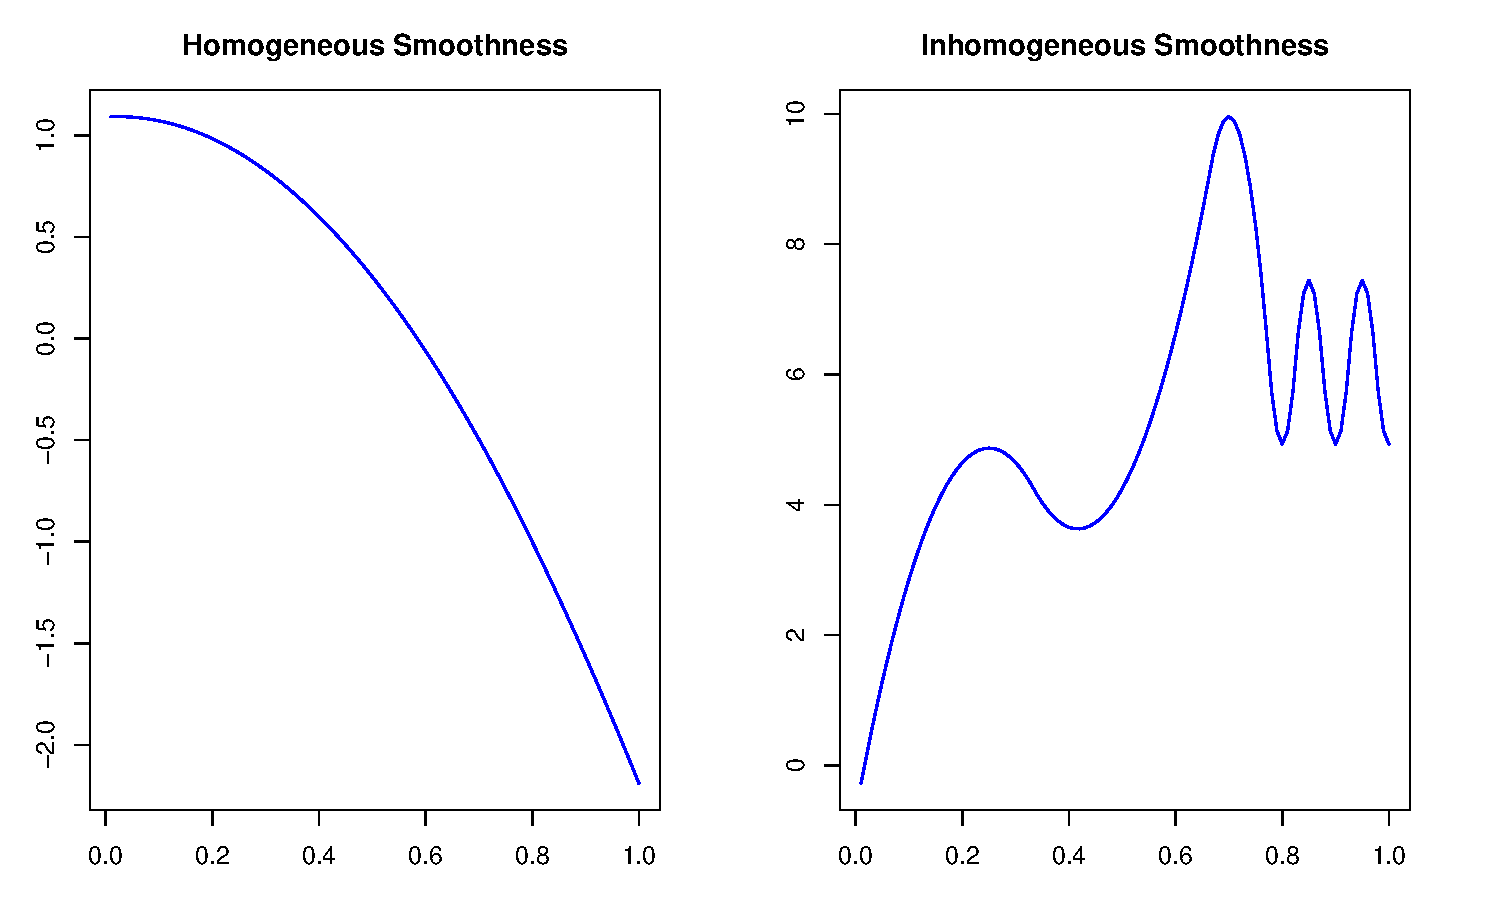
\includegraphics[width = 0.8\textwidth]{Figures/homo.pdf}
\caption{Left panel: a function with homogeneous smoothness. Right panel: a function with heterogeneous smoothness}
\label{fig:homo}
\end{figure}

From a theoretical point of view, linear smoothers have been proved to be sub-optimal for certain function class. In nonparametric estimation, we don't assume a parametric form of the true function $f_0$, but rather have a milder assumption that $f_0$ lies in some smooth function class. There are many notions of smoothness, some commonly used smooth function classes include: H\"older class $H(k)$, Sobolev class $\cal{W}(k)$, total variation class $\cal{F}(k)$, where $k$ refers to the order of smoothness usually expressed by assumptions on the $k$th derivative. Rigorous definitions of these function classes will be deferred to Section \ref{sec:theory}. One important result in minimax theory shows that under the $L_2$ risk, the minimax rate over the function class $\cal{F}(k)$ is $n^{-(2k+2)/(2k+3)}$\cite{donoho1998minimax}. However, when restricted to linear smoothers, the minimax rate is $n^{-(2k+1)/(2k+2)}$, i.e. any linear smoother can do no better than $n^{-(2k+1)/(2k+2)}$. This result demonstrates that linear smoothers are sub-optimal over functions whose derivatives are of bounded total variation. More explicitly, consider the case $k = 0$, i.e. the true function $f_0$ is of bounded total variation, for which the minimax convergence rate is $n^{-2/3}$. In such case, any linear smoother can do no better than $n^{-1/2}$, which means linear smoothers will still be consistent but at a much slower rate. See Figure \ref{fig:diagram} for a comparison of convergence rate for linear and nonlinear smoothers.

Defects of linear smoothers motivated the development of nonlinear smoothers. Before trend filtering, two most effective nonlinear smoothers are wavelet smoother\cite{johnstone2011gaussian,mallat2008wavelet,donoho1994ideal} and locally adaptive regression spline\cite{mammen1997locally}. Both methods have nice local adaptivity. In the top right panel of Figure \ref{fig:ssvslars}, locally adaptive spline accurately captures the "hills" on the right and successfully maintains the smoothness on the left. Moreover, both methods are theoretically appealing as have been proved to be minimax optimal over the bounded total variation class\cite{donoho1998minimax,mammen1997locally}. See again Figure \ref{fig:diagram} for the minimaxity of these two methods. These two methods are not perfect though. Generation of wavelet basis requires the inputs $(x_1, \ldots, x_n)$ to be evenly-spaced and sample size $n$ to be a power of 2, and there are often further assumptions made about the behavior of the fitted value at the boundaries of the input domain. Locally adaptive spline, on the other hand, is hard to solve in practice as there is no better alternative to solving a Lasso problem with dense design matrix, which takes $\cal{O}(n^3)$ operations. Moreover, to choose the locations of the knots in locally adaptive spline is usually hard for higher orders $k\geq 2$. Limitations of wavelet smoother and locally adaptive spline motivate us to look for a new nonlinear smoother, which is expected to be locally adaptive, computationally efficient and theoretically optimal in some sense.

\begin{figure}[t!]
\centering
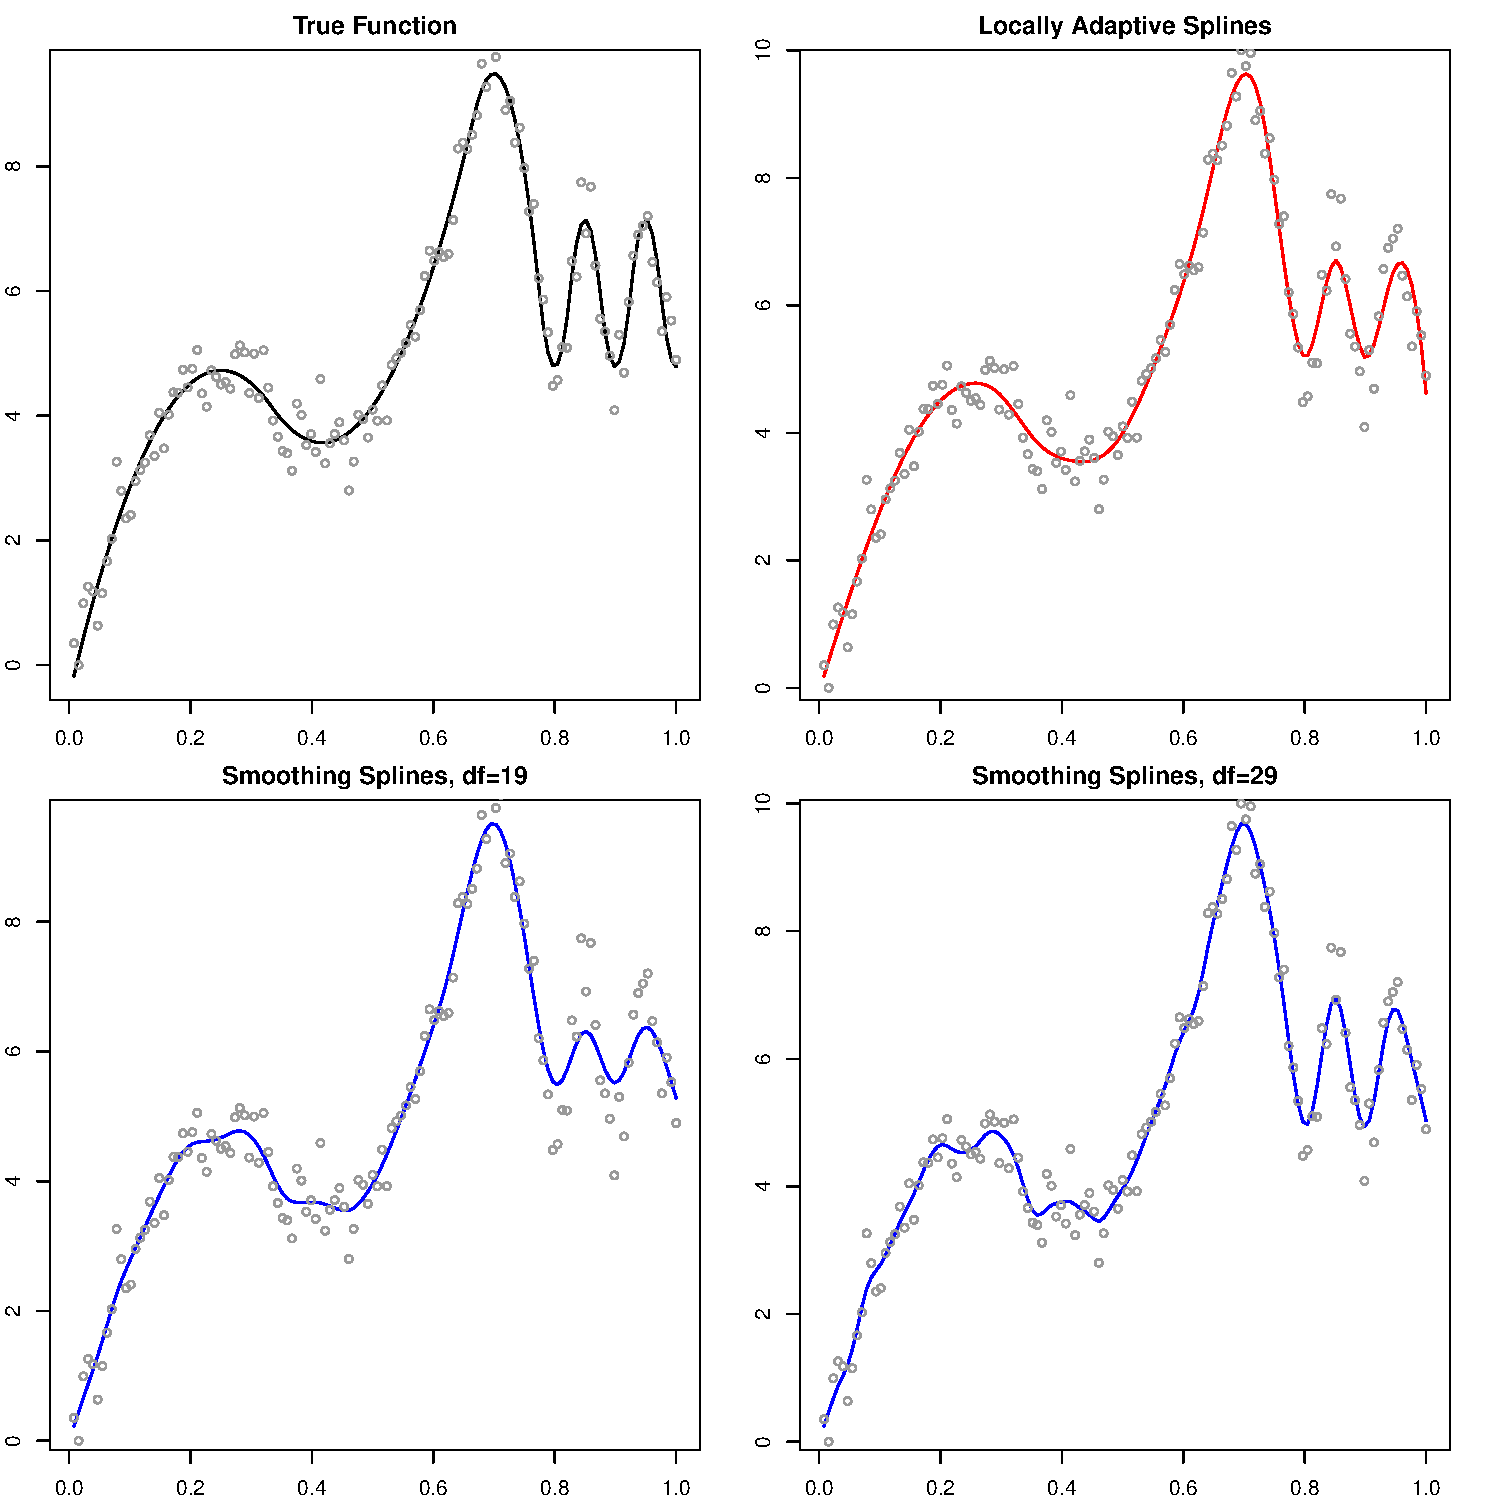
\includegraphics[width = 0.8\textwidth]{Figures/ssvslars.pdf}
\caption{Comparison of smoothing spline and locally adaptive spline over the "hills data". Top left panel shows the true function (black curve) with noisy observations (gray dots). Top right panel shows the fit of locally adaptive spline, which accurately captures the "hills" shape on the right and maintains smoothness on the left. The bottom panels show the fit of smoothing splines with 19 and 29 degrees of freedom respectively. The fit with small degrees of freedom over-smooth the "hills" shape while the fit with larger degrees of freedom suffers from under-smoothing issue on the left half.}
\label{fig:ssvslars}
\end{figure}

In this paper, we focus on one such method in the class of trend filtering estimators. Trend filtering, as its name suggests, was originally proposed to estimate the underlying trend in time series data, and had since then been applied in a variety of disciplines, such as economics \cite{hodrick1997postwar,tsay2005analysis}, astronomy \cite{kovacs2008application}, social science \cite{saha2012learning,levitt2004understanding}, medical science\cite{greenland1992methods,link1994estimating}, etc. A huge number of trend filtering estimators have been proposed, including moving averaging smoothing\cite{leser1961simple,kendall1946advanced,lucas1980two}, Hodrick-Prescott(H-P) filtering\cite{hodrick1997postwar},  smoothing splines\cite{de1978practical,wahba1990spline,green1993nonparametric}, etc. Most trend filtering estimators are based on $\ell_2$ regularization. H-P filtering, for example, directly penalizes the square of the second order difference of the estimate,

\begin{align}
\hat{u}^{\text{H-P}} \in \argmin_{u\in\RR^n} \frac{1}{2}\|y-u\|_2^2 +\lambda\sum_{i=2}^{n-1}(u_{i-1}-2u_i+u_{i+1})^2
\label{eq:HP}
\end{align}
where $y\in\RR^n$ is the observation signal of length $n$ and $\lambda$ is the tuning parameter. A relatively new trend filtering technique based on $\ell_1$ regularization was proposed in \cite{kim2009ell_1}, where the method solves the $\ell_1$ version of \eqref{eq:HP}

\begin{align}
\minimize_{u\in\RR^n} \frac{1}{2}\|y-u\|_2^2 + \lambda\sum_{i=2}^{n-1} |u_{i-1} - 2u_i + u_{i+1}| \label{eq:linear_tf}
\end{align}
Unlike the $\ell_2$ penalty, the $\ell_1$ penalty is sparsity-inducing and will render some entries of the discrete second-order difference zero. Zero-valued entries correspond to the smooth part of the estimate while non-zero entries correspond to wiggly part of the estimate, thus making the estimate locally adaptive. The new trend filtering technique discussed in this paper is a natural extension of \eqref{eq:linear_tf} and penalizes any order of discrete difference. Throughout the paper, we will work through and explore this more general version of $\ell_1$ trend filtering, and compare it with both linear and nonlinear smoothers. We will show that trend filtering is locally adaptive, can be solved by efficient algorithms and is minimax optimal over the bounded total variation class $\cal{F}(k)$.

\begin{figure}[t!]
\centering
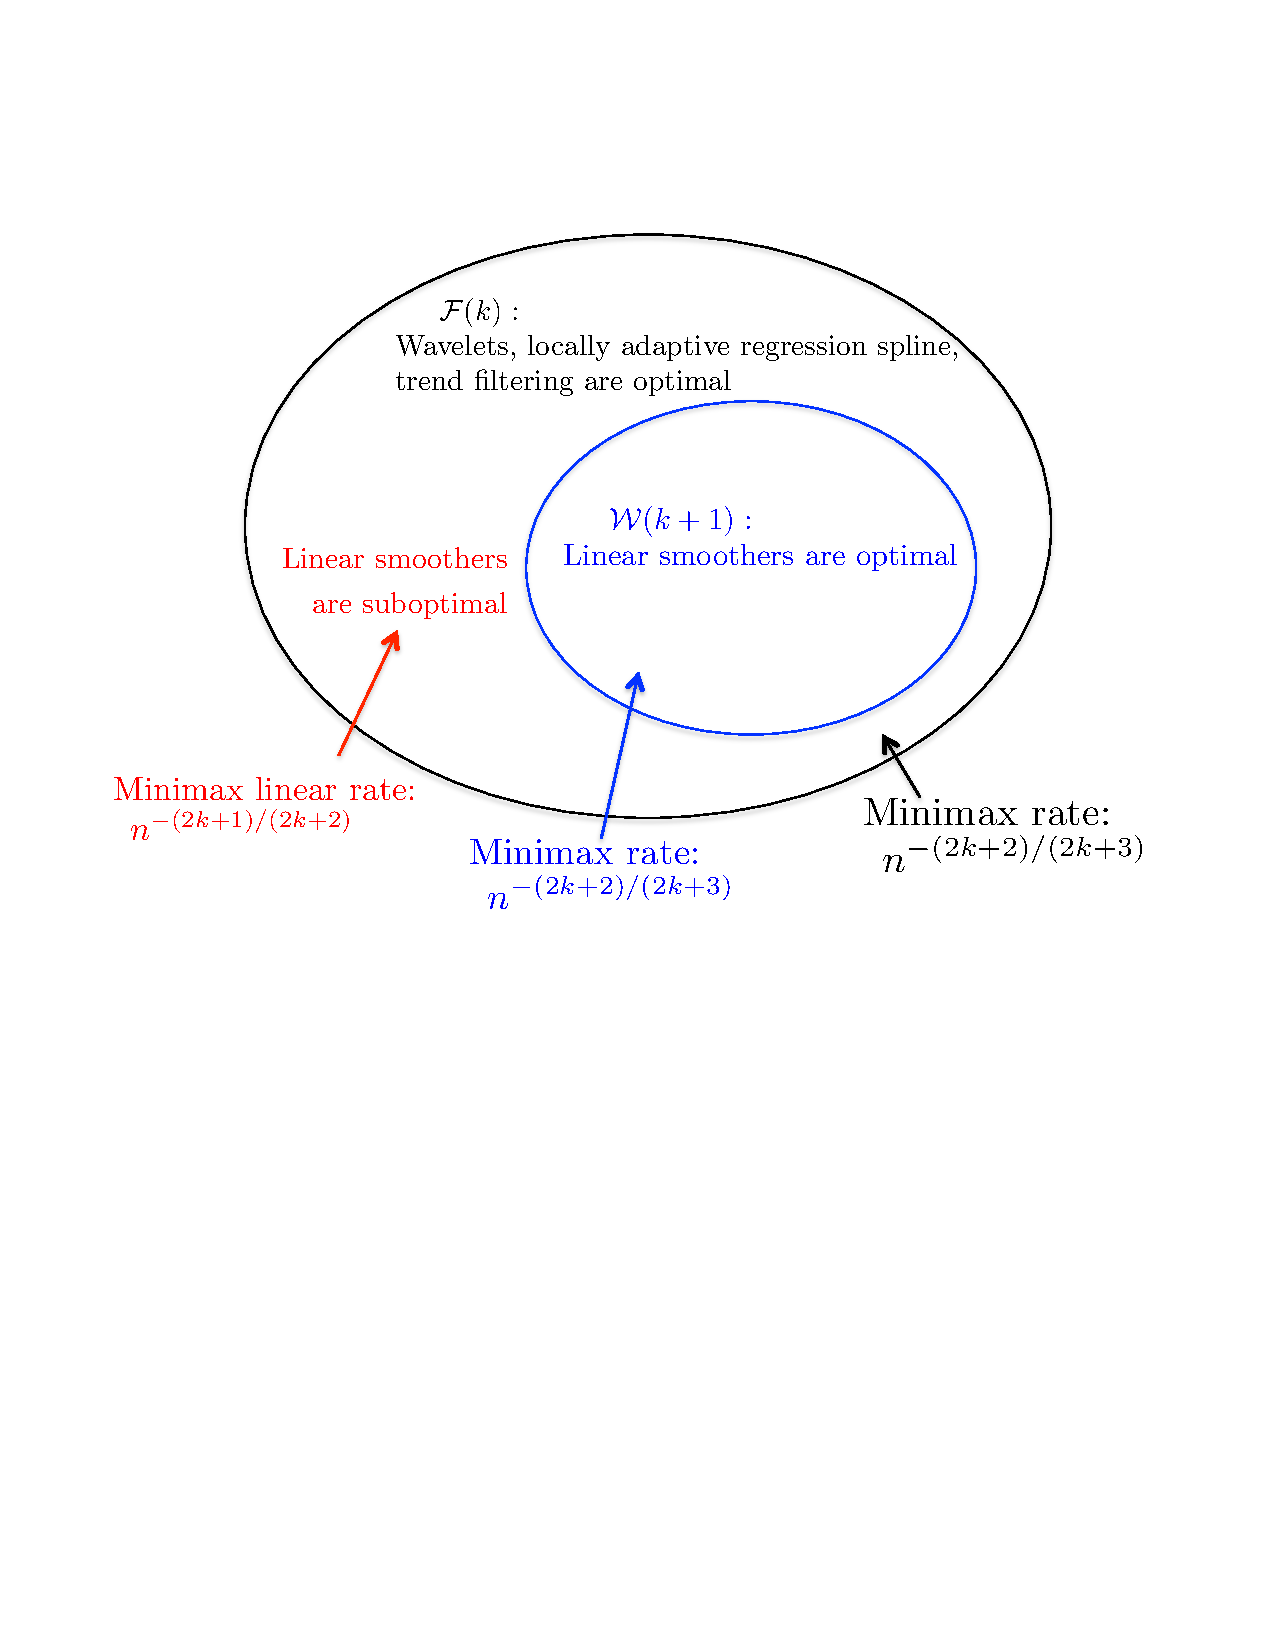
\includegraphics[width = 0.8\textwidth]{Figures/diagram.pdf}
\caption{Convergence rate of linear smoothers and nonlinear smoothers. The minimax rate over the $(k+1)$st order Sobolev class $\cal{W}(k+1)$ is $n^{-(2k+2)/(2k+3)}$, where wavelet method, locally adaptive spline, trend filtering and certain linear smoothers are optimal. However, when enlarged to the $k$th order bounded total variation class with the same minimax rate, the three nonlinear smoothers remain minimax optimal but all linear smoothers are sub-optimal and can do no better than $n^{-(2k+1)/(2k+2)}$ in this case.} 
\label{fig:diagram}
\end{figure}
 
It is worth mentioning that after this paper was published in 2014, there have been some exciting developments related to trend filtering. \cite{ramdas2016fast} proposed an efficient alternating direction method of multipliers (ADMM) algorithm to solve trend filtering and its variants (e.g. sparse trend filtering and mixed trend filtering introduced in Section \ref{subsec:syn_vs_ana}). \cite{wang2016trend} extended the notion of univariate trend filtering onto trend filtering on graphs and defined the discrete difference operator on graphs using the graph Laplacian matrix. \cite{sadhanala2017additive} and \cite{petersen2014fused} both extended trend filtering to high dimensions under the framework of additive model, while the latter focused on trend filtering of order $0$. \cite{wang2014falling} explored in depth the falling factorial basis used by the continuous-time representation of trend filtering. \cite{maidstone2017detecting} explored linear trend filtering ($k =1$) with $\ell_0$ penalty and proposed a novel dynamic-programming algorithm to solve the corresponding $\ell_0$ based optimization problem. 

The rest of the paper will be organized as follows. In Section \ref{sec:method}, we introduce the trend filtering estimator, develop its continuous representation and discuss several algorithms to solve it. We then compare trend filtering with smoothing spline and locally adaptive spline respectively in Section \ref{sec:comp_ss} and Section \ref{sec:las_compare}. In Section \ref{sec:real_data}  we consider three real datasets and compare trend filtering with smoothing spline and wavelet smoother. In Section \ref{sec:theory}, we derive the minimax convergence rate of trend filtering based on known results for locally adaptive spline. We then discuss some extensions of trend filtering in Section \ref{sec:extension} and conclude in Section \ref{sec:conclusion}. All the proofs are deferred to the Appendix, and at the end of the appendix we list out the possible errata of the original paper.


\section{Method}
\label{sec:method}

\subsection{Optimization Problem}
\label{subsec:opt_problem}
In this section, we generalize the $\ell_1$ trend filtering problem \eqref{eq:linear_tf} for higher orders. The $k$th order trend filtering is defined via the following optimization problem

\begin{align}
\minimize_{u\in\RR^n} \frac{1}{2}\|y-u\|_2^2 + \lambda\|D^{(k+1)}u\|_1  
\label{eq:tf}
\end{align}
where $y\in\RR^n$ is the observed noisy signal of length $n$ and $\lambda$ is the tuning parameter. For the rest of the paper, we will assume the signal $y$ to be observed at evenly-spaced time points $(x_1,\ldots, x_n)$. Note that this assumption is only for simplicity, a corresponding version for unevenly-spaced inputs is developed in Section \ref{subsec:uneven}. For the penalty term, $D^{(k+1)}\in\RR^{(n-k-1)\times n}$ is the $(k+1)$st order discrete difference operator. When $k = 0$, the difference operator $D^{(1)}$ in \eqref{eq:tf} is defined as

\begin{align}
D^{(1)} =
\begin{bmatrix}
-1 & 1 & 0 & \ldots & 0 & 0\\
0 & -1 & 1 & \ldots & 0 & 0\\
\vdots & \vdots & \vdots & \ddots & \vdots & \vdots\\
0 & 0 & 0 & \ldots & -1 & 1
\end{bmatrix}\in\RR^{(n-1) \times n}
\label{eq:D_0}
\end{align}
and therefore the penalty term in \eqref{eq:tf} becomes $\lambda\sum_{i=1}^{n-1}|u_{i+1}- u_i|$. This recovers as special case the 1d total-variation denoising problem \cite{rudin1992nonlinear,harchaoui2010multiple} and the fused-lasso problem with only the fused penalty term \cite{tibshirani2005sparsity}. For higher orders $k$, $D^{(k+1)}$ is recursively defined as

\begin{align}
D^{(k+1)} \equiv D^{(1)} \cdot D^{(k)} 
\label{eq:difference_op}
\end{align}
where $D^{(1)}$ is the $(n-k-1)\times (n-k)$ version of \eqref{eq:D_0}. The $(k+1)$st order difference operator therefore penalizes the change in the $k$th order difference. Note that when $k = 1$, the discrete difference operator $D^{(2)}$ is


\begin{align}
D^{(2)} =
\begin{bmatrix}
1 & -2 & 1 & 0 & \ldots & 0 & 0\\
0 & 1 & -2 & 1 & \ldots & 0 & 0\\
\vdots & \vdots & \vdots & \ddots & \vdots & \vdots & \vdots\\
0 & 0 & 0 & \ldots & 1 & -2 & 1
\end{bmatrix}\in\RR^{(n-2) \times n}
\end{align}

\begin{figure}[t!]
\centering
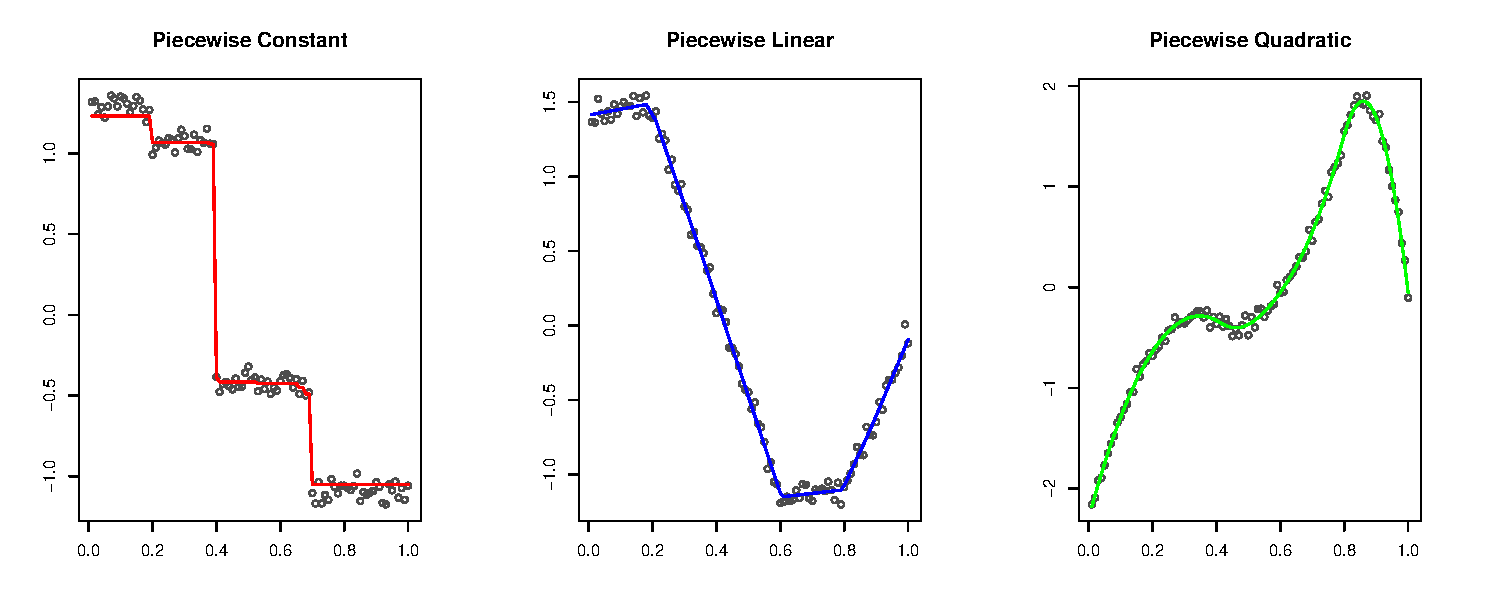
\includegraphics[width = 1\textwidth]{Figures/Figure1.pdf}
\caption{Examples of trend filtering of order $k =0, 1, 2$. The solution to \eqref{eq:tf} are only defined on the inputs $x_i = i/n$, $i=1,2,\ldots, n$, thus we use linear interpolation to display a "continuous" version of trend filtering. These estimates do seem to possess a piecewise polynomial structure.}
\label{fig:Figure1_examples}
\end{figure}

Without surprise, this recovers the linear trend filtering defined in \eqref{eq:tf}. Under the assumption that $y$ is observed at evenly-spaced time points $\{x_1,x_2,\ldots, x_N\}$, the definition in \eqref{eq:difference_op} can be seen as a discrete analogue of derivative. One might accordingly expect the $k$th order trend filtering estimator to behave somewhat similar to the $k$th order piecewise polynomials. Figure \ref{fig:Figure1_examples} gives some empirical evidence of this claim. From left to right, data are generated from true signals that are piecewise constant, piecewise linear and piecewise quadratic, and correspondingly we fit trend filtering of order $k = 0,1,2$. Note that the solution to \eqref{eq:tf} is only defined on the observed points $\{x_1,x_2, \ldots, x_n\}$, thus we use linear interpolation to display a "continuous" version of trend filtering, which does seem to possess a piecewise polynomial structure. This lead to two natural questions: is there a continuous representation $f$ of trend filtering, e.g. the solution $(\hat{u}_1,\ldots, \hat{u}_n)$ to \eqref{eq:tf} are evaluations of $f$ at $(x_1, x_2,\ldots, x_n)$? And if there is, if $f$ indeed a piecewise polynomial or spline? (Recall that $k$th order spline is $k$th order piecewise polynomial with continuous derivatives up to order $k-1$). For the first question, the answer is yes, and we will develop a continuous time representation of trend filtering in Section \ref{subsec:ct_tf}. For the second question, we will show in Section \ref{subsec:ct_tf} that for $k=0$ and $k=1$, the continuous representation $f$ of trend filtering is indeed spline; for $k\geq 2$, $f$ is piecewise polynomial but not spline, i.e. $f$ has discontinuous lower order derivatives. Before developing the continuous representation, we first introduce some basis properties of trend filtering.

\subsection{Trend Filtering as Lasso Type Problem}
\label{subsec:tfaslasso}
Recall that the generalized Lasso problem is defined as

\begin{align}
\minimize_{\beta\in\RR^p} \frac{1}{2}\|y-X\beta\|_2^2 + \lambda\|D\beta\|_1 
\label{eq:genlasso}
\end{align}
where $D\in\RR^{r\times p}$ is some general penalty matrix. In contrast to the ordinary Lasso problem, which directly penalizes the non-zero entries of $\beta$, the generalized Lasso induces sparsity on $D\beta$ to penalize some undesirable structure of $\beta$. By comparing \eqref{eq:tf} with \eqref{eq:genlasso}, we can see that $k$th order trend filtering is a generalized lasso problem with identity design and penalty matrix $D = D^{(k+1)}$, which indicates trend filtering enjoys many properties in Lasso type problems. One of the properties of interest is the degree of freedom, which we will use as a metric for model complexity to compare with other methods in later sections. \cite{tibshirani2011solution} fully characterized the degree of freedom in Lasso type problems, which gave rise to one unbiased estimator of the degree of freedom for \eqref{eq:tf} 

\begin{align}
\mbox{df}(\hat{u}) = \|D^{(k+1)}\hat{u}\|_0 + k + 1 \label{eq:dof}
\end{align}
where $\|\cdot\|_0$ is the number of nonzero entries. Note that $D^{(k+1)}$ takes the difference of $k$th order discrete difference, thus nonzero entries in $D^{(k+1)}\hat{u}$ correspond to knots or change points in the $k$th order discrete difference. \eqref{eq:dof} might seem strange in the first place, because the fit of $k$th order regression spline with the same knots has the same degree of freedom. Intuitively, trend filtering should have a larger degree of freedom than regression spline because it requires some extra degrees of freedom to locate those knots. However, the shrinkage of $D\hat{\beta}$ to zero in \eqref{eq:genlasso} counterbalances the extra degrees of freedom spent on the search, and the resulting degree of freedom is the same as the corresponding equality-constrained least square estimates. Such phenomenon is called the "over-shrinkage" property and also exists for ordinary Lasso. Figure \ref{fig:Figure2_overshrinkage} compares two different orders of trend filtering with corresponding regression spline with the same knots. Compared to regression spline, trend filtering shrinks the change of slope at knots in the linear case (left panel) and shrinks the curvature in the cubic case (right panel). Different orders of discrete differences of the cubic trend filtering estimate are shown in Figure \ref{fig:Figure3_discrete}. Again this empirically justifies the claim that the continuous representation of trend filtering is $k$th order piecewise polynomial because only the $3$rd derivative of cubic trend filtering is discontinuous and it is constant on the two segments separated by the knot.  

\begin{figure}[t!]
\centering
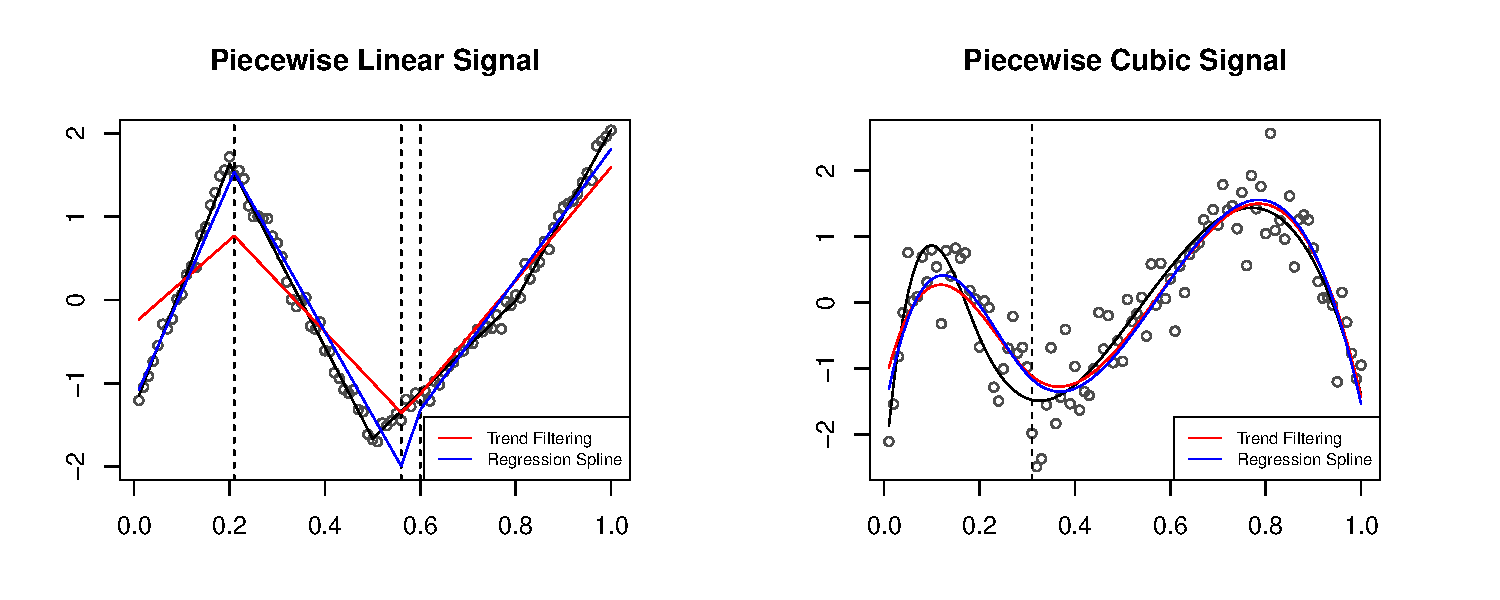
\includegraphics[width = 1.0\textwidth]{Figures/Figure2.pdf}
\caption{Comparison of linear and cubic trend filtering with corresponding regression splines with the same knots (vertical dashed lines). The "over-shrinkage" property of trend filtering can be seen in shrinking the change of slope in the linear case (left panel) and shrinking the curvature in the cubic case (right panel).}
\label{fig:Figure2_overshrinkage}
\end{figure}


\begin{figure}[t!]
\centering
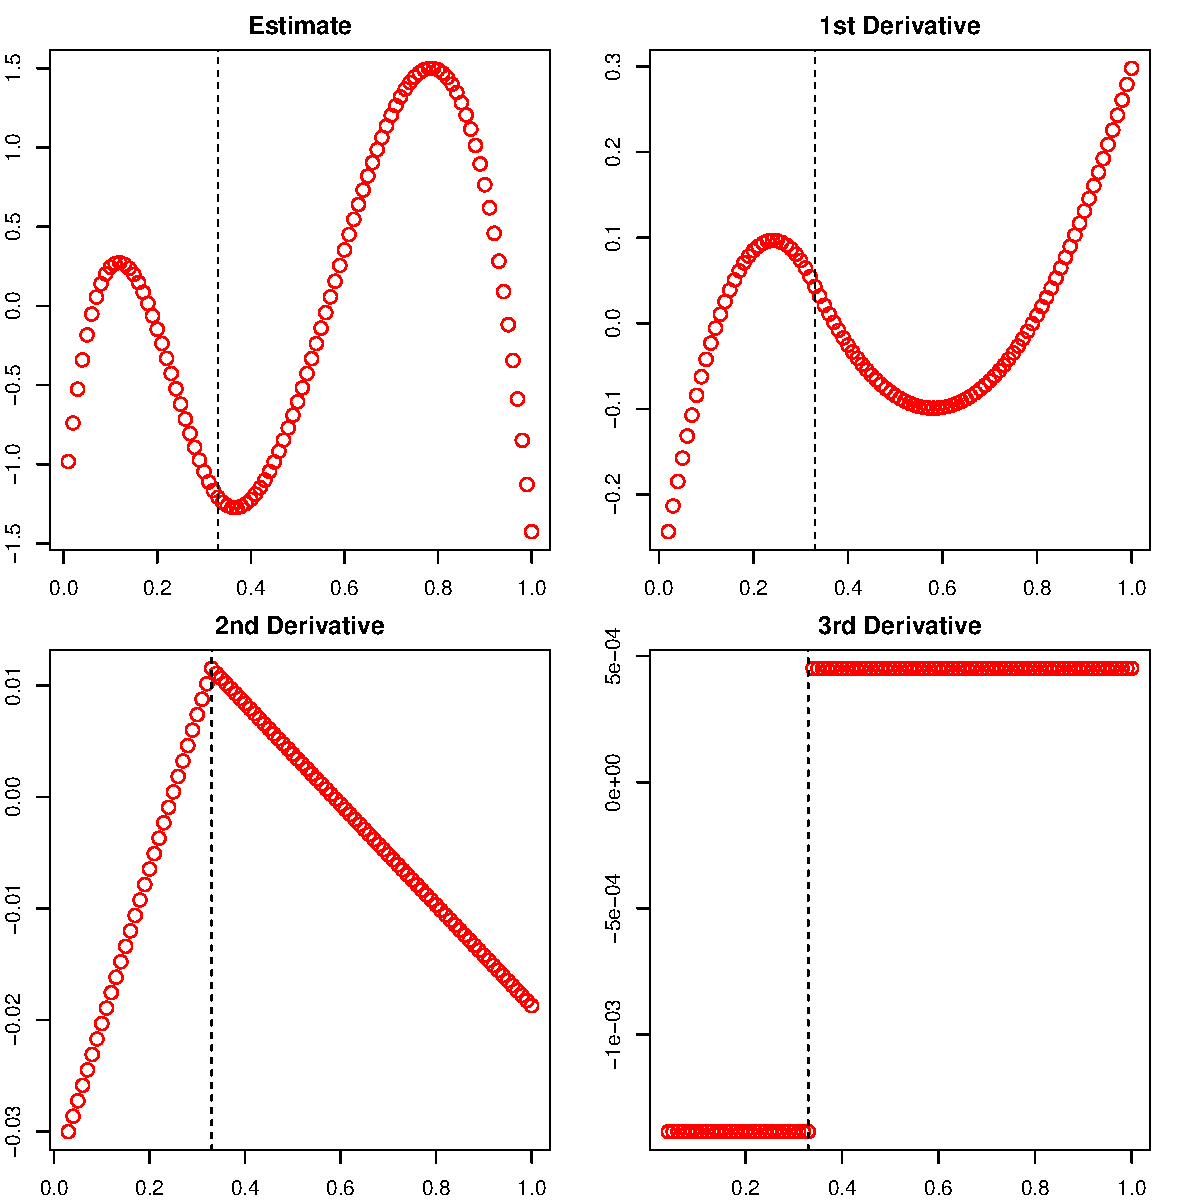
\includegraphics[width = 0.6\textwidth]{Figures/Figure3.pdf}
\caption{Function value, $1$st, $2$nd and $3$rd discrete difference of the cubic trend filtering estimate. Different orders of discrete difference are calculated by $D^{(k+1)}\hat{u}$ for $k=0,1,2$, where $\hat{u}$ is the solution to \eqref{eq:tf} with $k = 3$. The continuous function value, $1$st, $2$nd discrete difference and piecewise constant $3$rd discrete difference indicates the continuous representation of cubic trend filtering is a cubic piecewise polynomial.}
\label{fig:Figure3_discrete}
\end{figure}

\eqref{eq:genlasso} shows that trend filtering can be posed as a generalized Lasso problem. Notice the penalty matrix $D^{(k+1)}$ in trend filtering is a wide matrix, i.e. $D^{(k+1)}$ has more columns than rows and more importantly $D^{(k+1)}$ has full row rank for all $k$. This enables us to invert the penalty matrix and rewrite trend filtering as an ordinary Lasso problem. This is formalized in the following lemma.

\begin{lemma}
The trend filtering problem \eqref{eq:tf} is equivalent to the following Lasso problem
\begin{align}
\hat{\alpha} = \argmin_{\alpha\in\RR^n}\frac{1}{2}\|y-H\alpha\|_2^2 + \lambda\sum_{j=k+2}^n |\alpha_j|
\label{eq:tf_lasso}
\end{align}
in that the solution satisfies $\hat{u} = H\hat{\alpha}$. Here the design matrix $H\in\RR^{n\times n}$ is given by
\begin{equation}
H_{ij} = 
\begin{cases}
(\frac{i}{n})^{j-1}, & \text{for } i = 1,\ldots, n, j=1,\ldots, k+1\\
0, & \text{for } i \leq j-1, j\geq k+2\\
\sigma_{i-j+1}^{(k)} \cdot k!/n^k, &\text{for } i > j-1, j\geq k+2
\end{cases}
\label{eq:H_cumsum}
\end{equation}
where $\sigma_i^{(0)} = 1$ for all $i$ and
\begin{align*}
\sigma^{(k)}_i = \sum_{j=1}^i \sigma_j^{(k-1)}
\end{align*}
that is $\sigma_i^{(k)}$ is the $k$th order cumulative sum of $(1,1,\ldots, 1)\in\RR^i$.
\label{lemma:tf_lasso}
\end{lemma}
It is worth mentioning that \eqref{eq:tf_lasso} is a generalization for the case $k =1$ in Section 3.2 of \cite{kim2009ell_1}. Note that the design matrix in \eqref{eq:tf_lasso} is close to a lower-triangular matrix and thus has a sparse structure. This makes the general lasso solver very efficient in solving \eqref{eq:tf_lasso}. We will compare the Lasso solver with two other algorithms in Section \ref{subsec:algo}. 

\subsection{Continuous Representation of Trend Filtering}
\label{subsec:ct_tf}
The solution $\hat{u}$ to \eqref{eq:tf} is just a vector of discrete values at inputs $(x_1,\ldots, x_n)$ but doesn't tell us the exact form of our estimator $\hat{f}$ of the true regression function $f_0$. This is meaningless since we need to know the estimate at arbitrary point to make predictions. This motivates us to think about the following question: given the equivalent Lasso form \eqref{eq:tf_lasso}, is there a set of basis functions whose evaluations at inputs $(x_1,\ldots, x_n)$ give the design matrix $H$? The following lemma gives an affirmative answer.

\begin{lemma}
For evenly-spaced points $(x_1,\ldots, x_n)$, $x_i = \frac{i}{n}$ for $i=1,\ldots, n$, define the set of functions $(h_1, \ldots, h_n)$ such that
\begin{equation}
\begin{aligned}
h_1(x) = 1, \quad h_2(x) = x, \ldots, h_{k+1}(x) = x^k,\\
h_{k+1+j}(x) = \prod_{l=1}^k (x-x_{j+l})\mathbbm{1}_{[x\geq x_{j+k}]}, \quad \text{for } j = 1,\ldots, n-k-1
\label{eq:fall_fact}
\end{aligned}
\end{equation}
Then the design matrix $H$ in \eqref{eq:tf_lasso} is evaluation of $(h_1,\ldots, h_n)$ at $(x_1,\ldots, x_n)$, i.e.
\begin{align*}
H_{ij} = h_j(x_i) \quad i,j=1,\ldots, n
\end{align*}
\label{lemma:cont_tf}
\end{lemma}
Note that the basis functions $(h_1,\ldots, h_n)$ defined by \eqref{eq:fall_fact} are piecewise polynomial functions of order $k$. Consider the truncated power basis of the same order defined on $x_i = \frac{i}{n}$, $i= 1,\ldots, n$,
\begin{equation}
\begin{aligned}
g_1(x) = 1, \quad g_2(x) = x, \ldots, g_{k+1}(x) = x^k,\\
g_{k+1+j}(x) = (x-x_j)^k\mathbbm{1}_{[x\geq x_j]}, \quad \text{for }j=1,\ldots, n-k-1
\label{eq:trun_basis}
\end{aligned}
\end{equation}


\begin{figure}[t!]
\centering
   \begin{subfigure}[b]{1\textwidth}
   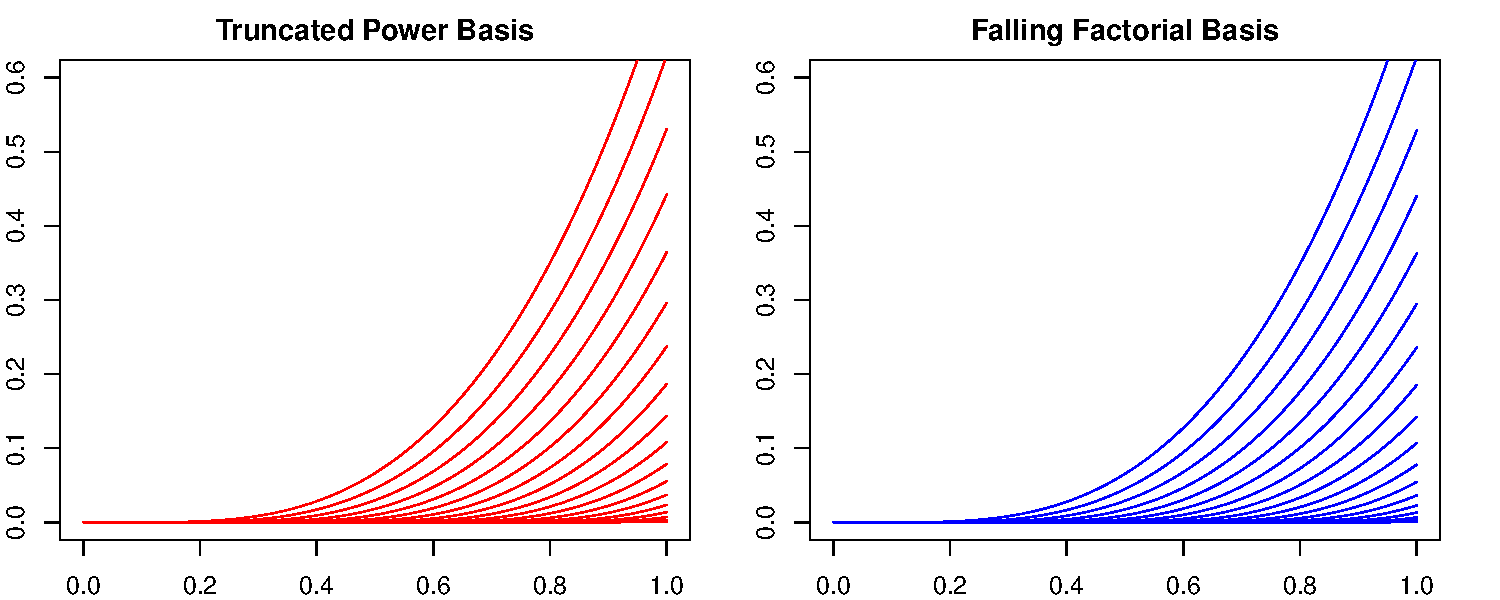
\includegraphics[width=1\linewidth]{Figures/Figure8.pdf}
   \caption{}
   \label{fig:8a}
\end{subfigure}

\begin{subfigure}[b]{1\textwidth}
   \includegraphics[width=1\linewidth]{Figures/Figure8b.pdf}
   \caption{}
   \label{fig:8b}
\end{subfigure}

\caption[Two numerical solutions]{(a) Comparison of truncated power basis and falling factorial basis of order $k=3$ over $n=22$ evenly-spaced inputs on $[0, 1]$. Visually truncated power basis (left panel) and falling factorial basis (right panel) are very similar. (b) Zoomed in parts of truncated power basis and falling factorial basis with same order and knots as (a). Truncated power basis has continuous $1$st and $2$nd derivatives, but the falling factorial basis has discontinuous first two derivatives.}
\label{fig:Figure8_fall}
\end{figure}


% \begin{figure}[t!]
% \centering
% 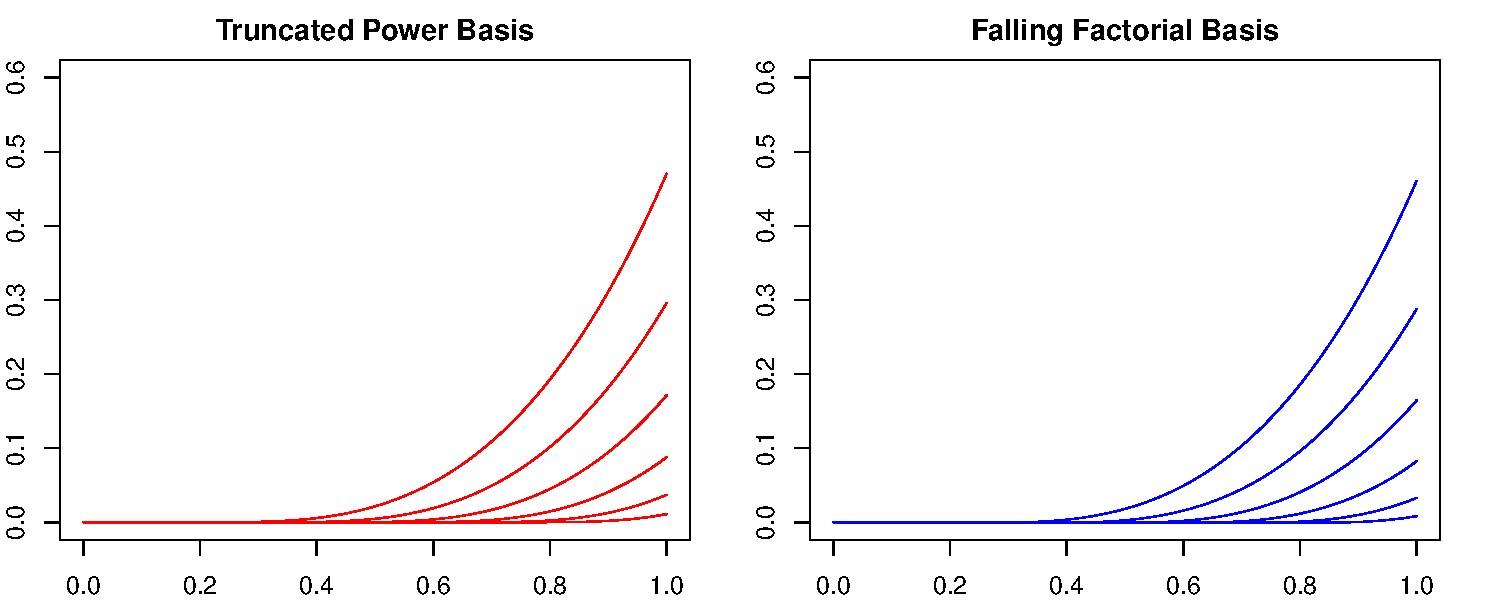
\includegraphics[width = 1\textwidth]{Figure8.pdf}
% \caption{Comparison of truncated power basis and falling factorial basis of order $k=3$. The left panel shows the truncated power basis \eqref{eq:trun_basis} and the right panel shows the falling factorial basis \eqref{eq:fall_fact}. Both sets of basis functions are defined over evenly-spaced $x_i = \frac{i}{n}$ for $i=1,\ldots, n$ with $n = 22$. Visually these two sets of functions are very similar.}
% \label{fig:Figure8_fall}
% \end{figure}

% \begin{figure}[t!]
% \centering
% \includegraphics[width = 1\textwidth]{Figure8b.pdf}
% \caption{Zoomed in parts of truncated power basis and falling factorial basis with same order and knots as Figure \ref{fig:Figure8_fall}. The left panel zooms in truncated power basis and the right panel zooms in the falling factorial basis. Truncated power basis has continuous derivative up to order 2, but the falling factorial basis has discontinuous first and second order derivatives.}
% \label{fig:Figure8b_fall}
% \end{figure}


Comparing \eqref{eq:fall_fact} and \eqref{eq:trun_basis}, we can see that these two sets of functions are extremely similar. In fact, the function set \eqref{eq:fall_fact} is called the falling factorial basis\cite{wang2014falling}, because each $h_{k+1+j}$ is the "falling" substitute of $g_{k+1+j}$ by replacing $(x-x_j)(x-x_j)\ldots(x-x_j)$ with $(x-x_{j+1})(x-x_{j+2})\ldots(x-x_{j+k})$. Figure \ref{fig:8a} compares the truncated power basis and falling factorial basis of order $k = 3$ over 22 evenly-spaced inputs on $[0, 1]$. We can see visually they are very similar. There is one nontrivial difference between these two sets though. It is well known that the $k$th order truncated power basis is a basis for regression spline, which means $g_i$, $i=1,\ldots, n$ are $k$th order splines. However, this is not true for the falling factorial basis. Figure \ref{fig:8b} zooms in parts of both basis sets. With $k =3$, truncated power basis has continuous $1$st and $2$nd derivative, while the falling power basis is continuous but has discontinuous first two derivatives.

The following lemma adopts the falling factorial basis \eqref{eq:fall_fact} to define a continuous representation of trend filtering:
\begin{lemma}
For inputs $x_1<\ldots<x_n$ and the basis functions $(h_1,\ldots, h_n)$ defined in \eqref{eq:fall_fact}, define the linear subspace of functions
\begin{align}
\cal{H}_k = \text{span}\{h_1,\ldots, h_n\} = \Big\{\sum_{j=1}^n \alpha_jh_j:\alpha_1,\ldots, \alpha_n\in\RR\Big\}
\label{eq:linear_class}
\end{align}
If the inputs are evenly-spaced, $x_i=\frac{i}{n}$ for $i=1,\ldots, n$, then the continuous minimization problem
\begin{align}
\hat{f} = \argmin_{f\in\cal{H}_k} \frac{1}{2}\sum_{i=1}^n(y_i-f(x_i))^2 + \lambda\cdot\text{TV}(f^{(k)})
\end{align}
is equivalent to the trend filtering problem \eqref{eq:tf} in that their solutions are the same at inputs.
\begin{align*}
\hat{u}_i = \hat{f}(x_i) \quad \text{for } i=1,\ldots,n  
\end{align*}
\label{lemma:cont}
\end{lemma}

Despite the original formulation of trend filtering in \eqref{eq:tf} is discrete in nature, Lemma \ref{lemma:cont} nicely characterizes a continuous representation of trend filtering, which facilitates the comparison with other function estimation technique, such as smoothing spline and locally adaptive regression spline. Moreover, since the falling factorial basis \eqref{eq:fall_fact} has discontinuous lower-order derivative for $k\geq 2$, Lemma \ref{lemma:cont} concludes that for $k = 0,1$, the continuous representation of trend filtering is piecewise constant and linear spline respectively; for $k\geq 2$, the fit of continuous trend filtering is piecewise polynomial but not spline.

\subsection{Algorithms}
\label{subsec:algo}
The Lasso form \eqref{eq:tf_lasso} and generalized Lasso form \eqref{eq:genlasso} motivate the following algorithms to solve the trend filtering problem \eqref{eq:tf}. 

\textbf{Algorithm I} The first algorithm solves the Lasso problem \eqref{eq:tf_lasso}. Notice that \eqref{eq:tf_lasso} is not a standard Lasso problem because the $\ell_1$ penalty does not penalize the first $(k+1)$ entries. However, we could first solve the first $(k+1)$ entries in terms of the rest, then solve the standard Lasso problem. More specifically, write $H = [H_1,H_2], \alpha = [\alpha_1, \alpha_2]$, such that $H_1$ and $\alpha_1$ refers to the first $(k+1)$ columns of $H$ and first $(k+1)$ entries of $\alpha$ respectively. Now take the derivative of the objective function in \eqref{eq:tf_lasso} with respect to $\alpha_1$ and set it to zero, we obtain

\begin{align}
\hat{\alpha}_1 = (H_1^TH_1)^{-1}H_1^T(y-H_2\alpha_2) 
\label{eq:algo_lasso}
\end{align}
Now plug \eqref{eq:algo_lasso} into \eqref{eq:tf_lasso}, we obtain the standard-form Lasso problem

\begin{align}
\hat{\alpha}_2 = \argmin_{\alpha_2\in\RR^{n-k-1}} \frac{1}{2}\|\tilde{y} - \tilde{X}\alpha_2\|_2^2 + \lambda\|\alpha_2\|_1
\label{eq:algo_lasso2}
\end{align}
where $\tilde{y} \equiv (\mathbb{I}_n - H_1(H_1^TH_1)^{-1}H_1^T)y$ and $\tilde{X} \equiv (\mathbb{I}_n - H_1(H_1^TH_1)^{-1}H_1^T)H_2$. The solution for \eqref{eq:tf_lasso} thus becomes 
\begin{align}
\hat{\alpha} = ((H_1^TH_1)^{-1}H_1^T(y-H_2\hat{\alpha}_2), \hat{\alpha}_2)
\end{align}
The computational cost for solving $\alpha_1$ is $\cal{O}(nk^2)$, and solving Lasso problem \eqref{eq:algo_lasso2} using, for example, least angle regression\cite{efron2004least} requires $\cal{O}(k^3 + nk+2)$. For $k\leq n$, this requires $\cal{O}(nk^2)$ operations in total to solve the trend filtering problem for one $\lambda$. The \textit{lars} R package solves \eqref{eq:algo_lasso} for all $\lambda$ values and the \textit{glmnet} R package solves \eqref{eq:algo_lasso2} for a sequence of $\lambda$ values.

\textbf{Algorithm II} The second algorithm is the path algorithm for solving generalized Lasso problem \cite{harchaoui2010multiple,tibshirani2011solution}. This algorithm solves the dual problem of \eqref{eq:genlasso}, which after some simple algebra gives

\begin{equation}
\begin{aligned}
&\minimize_{u\in\RR^m} \frac{1}{2}\|y-D^Tu\|_2^2\\
&\mbox{subject to } \|u\|_\infty \leq \lambda
\label{eq:algo_dual}
\end{aligned}
\end{equation}
where $m$ is the number of rows of $D$. The path algorithm starts from $\lambda = \infty$ and solves \eqref{eq:algo_dual} for all $\lambda$ values. After obtaining the solution $\hat{u}$ to \eqref{eq:algo_dual}, the primal solution can be recovered by $y - D^T\hat{u}_\lambda$.
The solution $\hat{u}_\lambda$ indexed by $\lambda$ is a piecewise linear function with respect to $\lambda$. The computational cost for each critical point in the path is $\cal{O}(n)$, and in practice the solution path may contain larger than $n$ critical points. The \textit{genlasso} R package provides efficient implementation of this algorithm.

\textbf{Algorithm III} The third algorithm also solves the dual problem \eqref{eq:algo_dual} instead of the primal problem, using an interior point algorithm. Such algorithm was first proposed in \cite{kim2009ell_1} to solve linear trend filtering problem but can be easily extended to higher orders. Each iteration of the primal-dual interior point algorithm takes $\cal{O}(n)$ operations and the worst-case scenario takes $\cal{O}(n^{1/2})$ iterations, thus overall the worst-case computation cost is $\cal{O}^{3/2}$ to solve for a single $\lambda$. However, the authors report that in practice the number of iterations is only a few tens and is nearly independent of the sample size $n$, thus the practical computation cost is close to $\cal{O}(n)$. Efficient implementation in C and Matlab can be found at \url{http://stanford.edu/~boyd/l1_tf}. 

Since the most commonly used order for trend filtering is $k = 3$, we compare the performance of \textbf{Algorithm I} using the \textit{lars} R package and \textbf{Algorithm II} using the \textit{trendfilter} function in \textit{genlasso} package. We test a case with $n = 1000$ data points on a standard laptop. \textbf{Algorithm I} takes about 14 seconds for $4018$ $\lambda$ values, and \textbf{Algorithm II} takes 19 seconds for $4239$ critical points. The \textit{lars} package is relatively faster. 


\section{Comparison with Smoothing Spline}
\label{sec:comp_ss}
Smoothing spline is an extremely popular tool in nonparametric function estimation. It has more flexibility compared to regression spline because it circumvents the problem of knot selection (as they just use the inputs as knots). Smoothing spline was originally motivated and defined from a functional minimization perspective. Given inputs $(x_1,\ldots, x_n)$ lying in an interval, say $[0, 1]$, the smoothing spline estimate $\hat{f}$ of a given odd integer order $k\geq 0$ is defined as

\begin{align}
\hat{f} = \argmin_{f\in\cal{W}_{(k+1)/2}}\sum_{i=1}^n (y_i - f(x_i))^2 + \lambda \int_0^1 (f^{((k+1)/2)}(t))^2dt
\label{eq:ss}
\end{align}
where $f^{((k+1)/2)}(t)$ the $((k+1)/2)$nd derivative of $f$ and the function class $\cal{W}_{(k+1)/2}$ is the $((k+1)/2)$nd order Sobolev space defined as

\begin{align*}
\cal{W}_{(k+1)/2} = \big\{f:[0,1]\rightarrow \RR:f\text{ is (k+1)/2 times differentiable with } \int_0^1(f^{((k+1)/2)}(t))^2dt<\infty\big\}
\end{align*}
\eqref{eq:ss} is an infinite-dimensional optimization problem over all functions $f$ in the $((k+1)/2)$nd order Sobolev space. This optimization criterion trades off the least squares error of $f$ over the observed pairs $(x_i, y_i)$, $i=1,\ldots, n$, with a penalty term that is large when the $((k+1)/2)$nd derivative of $f$ is wiggly. The tuning parameter $\lambda \geq 0$ governs the strength of each term in the minimization. Note that in order for the definition \eqref{eq:ss} to be valid, $k$ must be an odd integer. In practice, the most commonly used order is $k = 3$, i.e. cubic smoothing spline. 

Despite the infinite-dimensional nature in \eqref{eq:ss}, we will show in the next paragraph that smoothing spline has the so called \textit{variational} property which will aid in its solution. Roughly speaking, this property indicates that the best interpolant of \eqref{eq:ss}, i.e. the function with the smallest derivative penalty $\int_0^1(f^{((k+1)/2)}(t))^2dt$ among all those matching function values at inputs $(x_1,\ldots, x_n)$ is a natural spline of order $k$ with knots located at each distinct value of $(x_1,\ldots, x_n)$. This remarkable property of smoothing spline reduces \eqref{eq:ss} to a finite-dimensional problem and makes computation for smoothing spline extremely efficient.

\subsection{Variational Property}
\label{subsec:var_property}
It can be proved (see e.g. Exercise 5.7 of \cite{friedman2001elements}) that the solution to \eqref{eq:ss} is a natural spline of order $k$ with knots located at distinct values of $(x_1,\ldots, x_n)$. This is called the \textit{variational} property of smoothing spline\cite{anselone1968general}. Easy calculation shows that the space of $k$th order natural spline on $n$ distinct inputs has $n$ basis functions. Consider such a basis $(\eta_1,\ldots, \eta_n)$, let matrix $N\in\RR^{n\times n}$ be the evaluation of $\eta_1,\ldots, \eta_n$ at inputs $(x_1,\ldots, x_n)$ and $\Omega$ contains the integrated products of the $((k+1)/2)$nd derivative of $(\eta_1,\ldots, \eta_n)$, i.e.
\begin{align}
N_{ij} = \eta_j(x_i), \quad \Omega_{ij} = \int_0^1 \eta_i^{((k+1)/2)}(t)\eta_j^{((k+1)/2)}(t)dt \quad i,j=1,\ldots,n
\label{eq:ss_N}
\end{align}
then the infinite-dimensional problem \eqref{eq:ss} can be written more succinctly as

\begin{align}
\hat{\beta} = \argmin_{\beta\in\RR^n} \|y-N\beta\|_2^2 + \lambda\beta^T\Omega\beta
\label{eq:ss_ridge}
\end{align}
showing the smoothing spline problem to be a type of generalized ridge regression problem. In fact, \eqref{eq:ss_ridge} has the closed-form solution
\begin{align}
\hat{\beta} = (N^TN + \lambda\Omega)^{-1}N^Ty
\end{align}
and therefore the fitted values $\hat{\mu} = (\hat{f}(x_1),\ldots, \hat{f}(x_n))$ are
\begin{align}
\hat{\mu} = N(N^TN + \lambda\Omega)^{-1}N^Ty
\label{eq:ss_sol}
\end{align}
Smoothing spline therefore is a type of linear smoother with smoothing matrix $S_\lambda = N(N^TN + \lambda\Omega)^{-1}N^T$ and corresponding degree of freedom $\mbox{df}(\hat{f}) = \mbox{tr}(S_\lambda)$. It is informative to write \eqref{eq:ss_sol} as what is called the Reinsch form,

\begin{equation}
\begin{aligned}
\hat{\mu} &= N(N^TN + \lambda\Omega)^{-1}N^Ty\\
&= N(N^T(I + \lambda (N^T)^{-1}\Omega N^{-1})N)^{-1}N^Ty\\
&= (\mathbb{I}_n + \lambda Q)^{-1}y
\end{aligned}
\label{eq:ss_reinsch}
\end{equation}
where $Q =(N^T)^{-1}\Omega N^{-1}$. Note that $Q$ does not depend on $\lambda$. If we compute its eigen-decomposition as $Q = UDU^T$ with each column of $U$ denoted by $u_j$, $j=1,\ldots, n$ and $D$ as $\mbox{diag}(d_1,\ldots, d_n)$, the the eigen-decomposition of the smoothing matrix $S_\lambda$ is 

\begin{align*}
S_\lambda = \sum_{j=1}^n \frac{1}{1+\lambda d_j}u_ju_j^T
\end{align*}
therefore the smoothing spline fitted value $\hat{\mu}$ is 

\begin{align}
\hat{\mu} = \sum_{j=1}^n \frac{u_j^Ty}{1+\lambda d_j}u_j
\label{eq:ss_fit}
\end{align}
\eqref{eq:ss_fit} shows that smoothing spline actually regresses on the orthonormal basis $(u_1,\ldots, u_n)$, yet they shrink the coefficients in this regression with more shrinkage assigned to eigen-vectors $u_j$ that correspond to larger eigenvalues $d_j$. The basis $(u_1,\ldots, u_n)$ are named \textit{Demmler-Reinsch} basis\cite{demmler1975oscillation}. Roughly speaking, eigen-vectors $u_j$ that correspond to smaller $d_j$ are smoother, thus are penalized less. On the contrary, $u_j$ corresponding to more wiggly components endure larger penalization. 

Now to compare with the formulation of trend filtering, the transformation $\hat{\mu} = N\hat{\beta}$ can be seen as the solution to the minimization problem

\begin{equation}
\begin{aligned}
\hat{\mu} &= \argmin_{u\in\RR^n} \|y-u\|_2^2 + \lambda u^TQu\\
&= \argmin_{u\in\RR^n} \|y-u\|_2^2 + \lambda\|Q^{1/2}u\|_2^2
\label{eq:ss_newform}
\end{aligned}
\end{equation}
Note that \eqref{eq:ss_newform} is extremely similar to the original formulation of trend filtering \eqref{eq:tf}. One difference is that $Q^{1/2}$ is generically different from the penalty matrix $D^{(k+1)}$ in \eqref{eq:tf}. More importantly, \eqref{eq:ss_newform} is coupled with square $\ell_2$ norm while \eqref{eq:tf} is penalized by $\ell_1$ norm. It is well-known that $\ell_1$ is a sparsity-inducing norm and $\ell_2$ isn't. Accordingly, one might expect the superiority of Lasso regression over ridge regression will carry over to this setting, making trend filtering more locally adaptive than smoothing spline. Simulation in the next subsection will empirically support this claim, and we will further analyze and compare the convergence rate of linear smoothers and nonlinear smoothers in Section \ref{sec:theory}.

\subsection{Empirical Comparison}
\label{subsec:sssimu}
\begin{figure}[t]
\centering
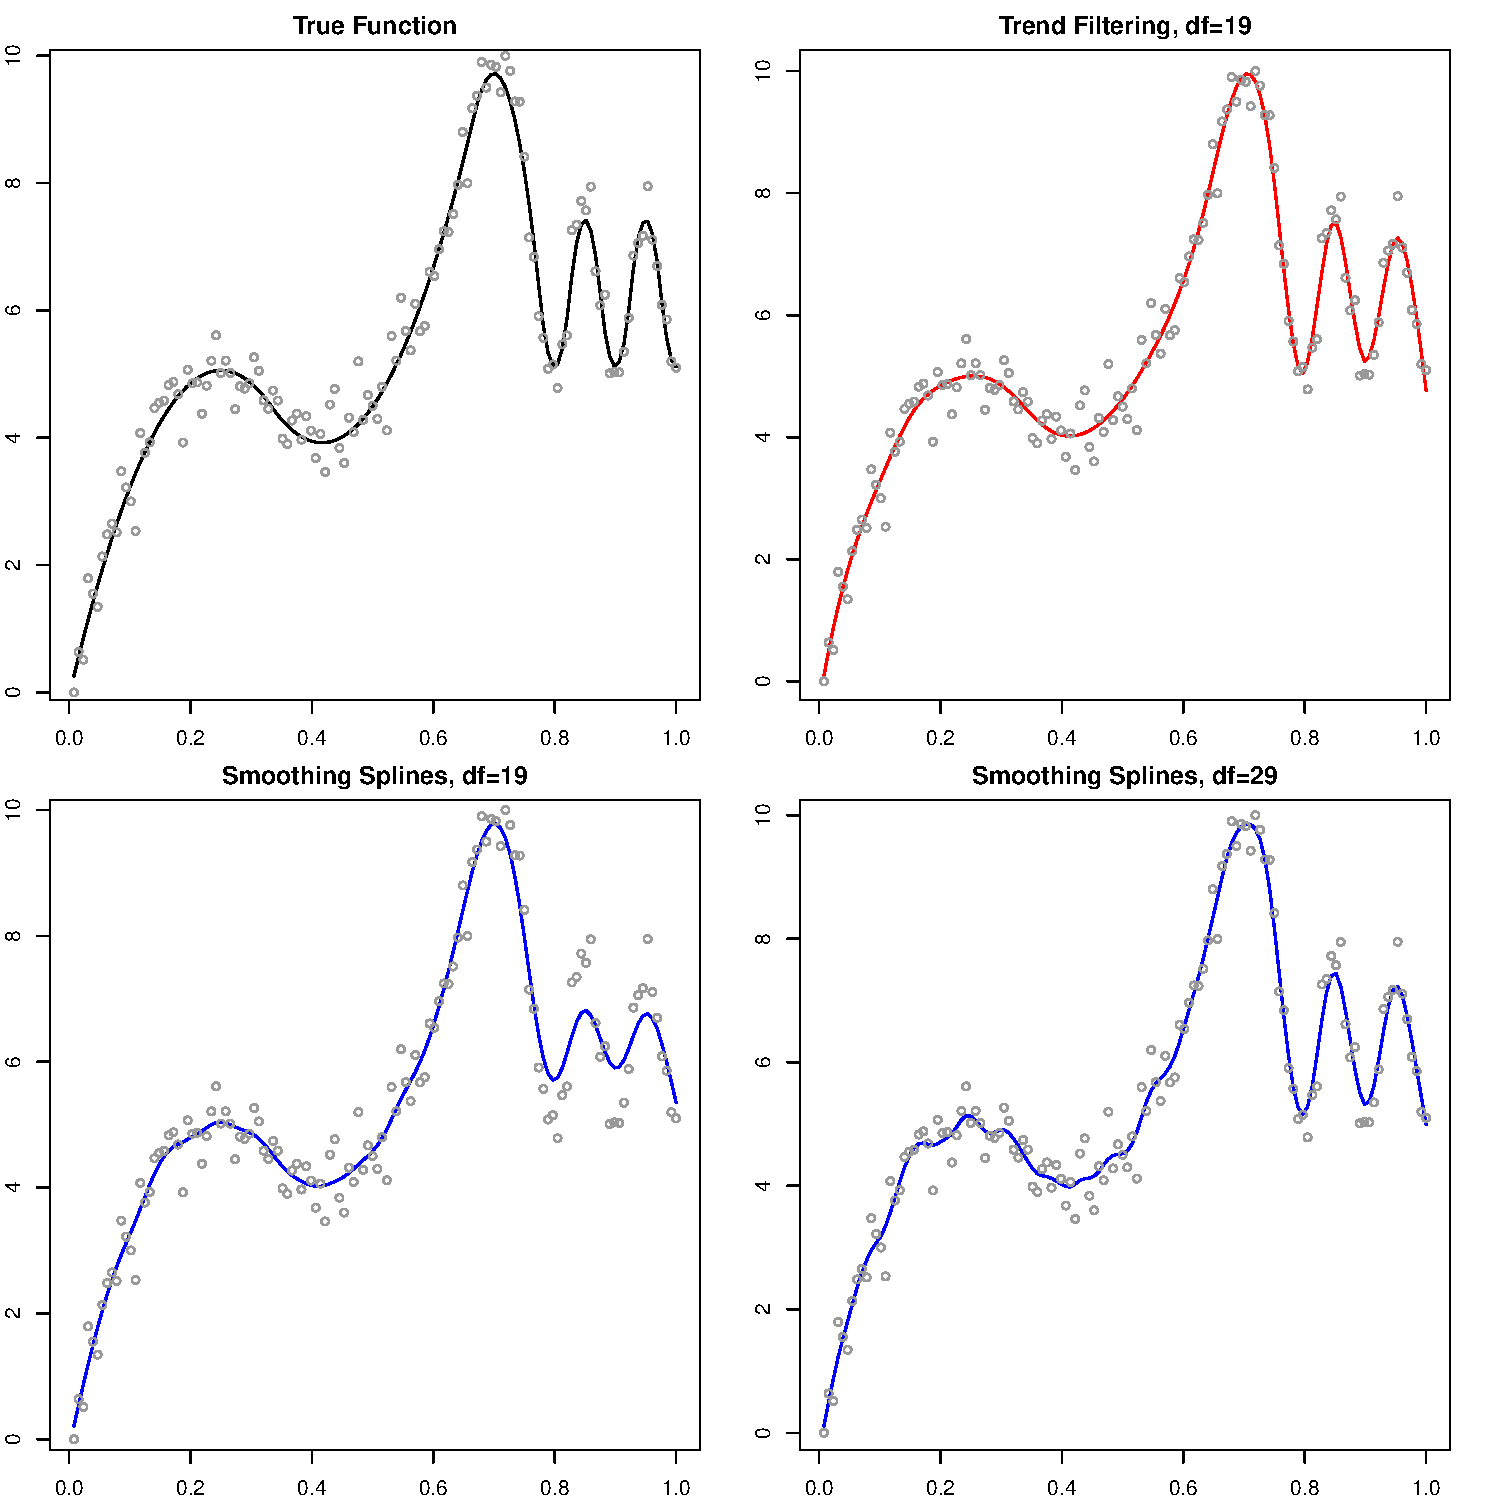
\includegraphics[width = 0.6\textwidth]{Figures/Figure4.pdf}
\caption{Comparison of trend filtering and smoothing spline over the same "hills" data consider in Figure \ref{fig:ssvslars}. The trend filtering fit with $df = 19$ (top right panel) clearly outperforms both smoothing spline estimates.}
\label{fig:Figure4_ssvstfhills}
\end{figure}

We will compare trend filtering and smoothing spline of order $k = 3$. For cubic smoothing spline, the \textit{smooth.spline} function in R is extremely fast. To demonstrate trend filtering is more locally adaptive than smoothing spline, we will compare these two methods over two  simulated data sets generated from heterogeneous signals: the "hills" data in the top left panel of Figure \ref{fig:ssvslars}, and the Doppler signal. 


The estimates of cubic smoothing spline and cubic trend filtering over the "hills" data  is shown in Figure \ref{fig:Figure4_ssvstfhills}. The defect of smoothing spline has been shown in the Section \ref{sec:intro}. The fit of trend filtering with 19 degrees of freedom accurately captures the "hills" shape on the right while successfully maintaining the smoothness on the left. It adapts better to the varying level of smoothness than smoothing spline.

\begin{figure}[t]
\centering
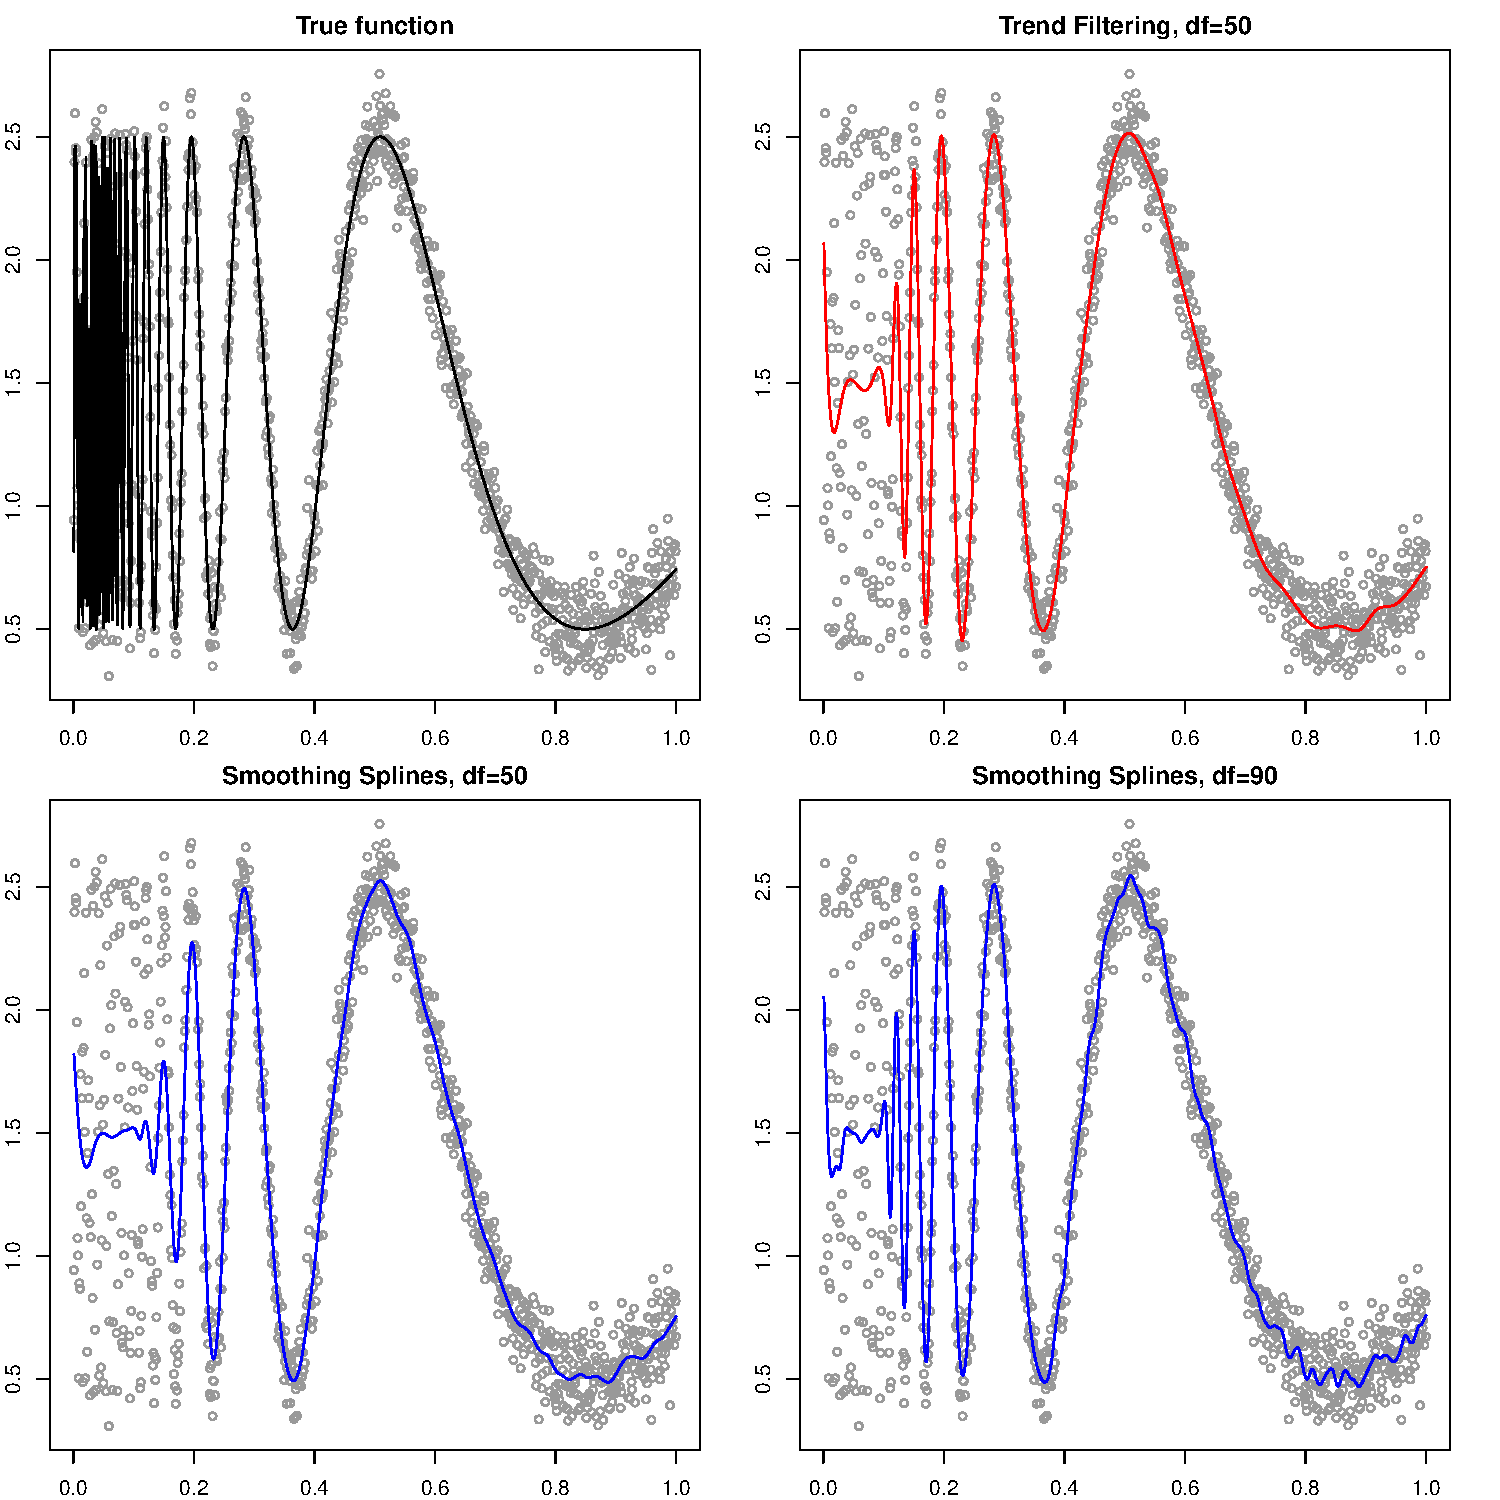
\includegraphics[width = 0.6\textwidth]{Figures/Figure5.pdf}
\caption{Comparison of trend filtering and smoothing spline over the heterogeneous Doppler signal. Top left panel: true function with $n = 1000$ noisy observations; top right panel: trend filtering fit with 50 degrees freedom; bottom left panel: smoothing spline with 50 degrees of freedom; bottom right panel: smoothing spline with 90 degrees of freedom. With 50 degrees of freedom, trend filtering captures 4 cycles of oscillations on the left while smoothing spline only captures. When degree of freedom is increased to 90 to allow for more flexibility, smoothing spline finally picks up 4 cycles on the left but at the price of being severely wiggly near the right boundary.}
\label{fig:Figure5_ssvstfdoppler}
\end{figure}

We then compare smoothing spline and trend filtering on another well-known heterogeneous signal--- the Doppler signal. The true function with noise observations is shown in the top left panel of Figure \ref{fig:Figure5_ssvstfdoppler}. The signal can be seen to be highly heterogeneous in terms of smoothness. The left part of the functions exhibits high-frequency oscillations while the right low-frequency part is relatively smooth. In the top right panel is the fit of cubic trend filtering with 50 degrees of freedom, which picks up 4 cycles of oscillations on the left and remains sufficiently smooth in the low-frequency area. Smoothing spline with 50 and 90 degrees of freedom are shown in the bottom panels. With 50 degrees of freedom (same as trend filtering), smoothing spline only recovers 3 cycles in the high-frequency area. When increased to 90 degrees of freedom, the smoothing spline estimate finally recovers 4 cycles on the left but becomes extremely wiggly on the right. 

\begin{figure}[t]
\centering
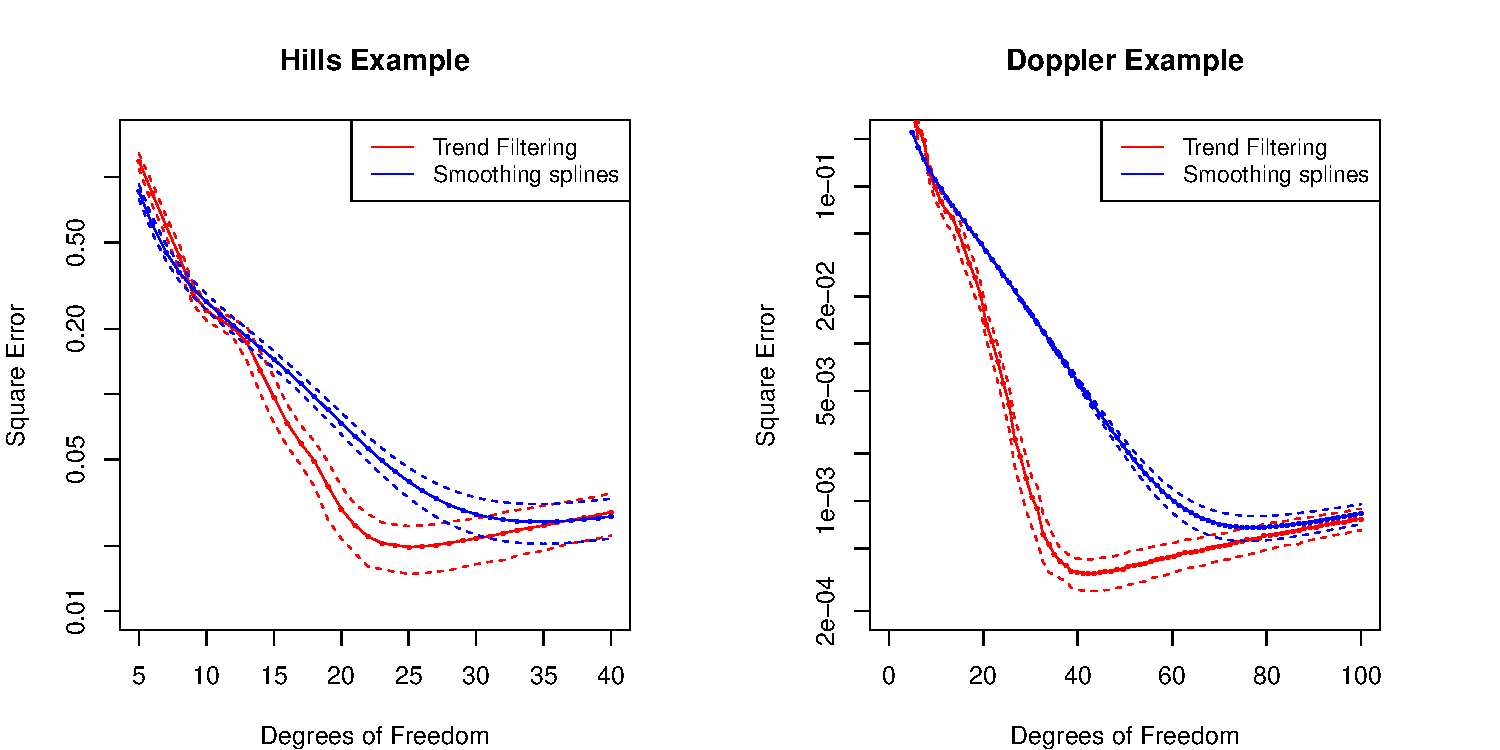
\includegraphics[width = 0.8\textwidth]{Figures/Figure6.pdf}
\caption{Comparison of cubic trend filtering and cubic smoothing spline in terms of MSE over the "hills" data (left panel) and the Doppler example (right panel). In each setup, trend filtering and smoothing spline estimators were fit over a range of degrees of freedom values. The red curves display the loss for trend filtering, and the blue curves for smoothing spline. The results were averaged over 50 simulated data sets, and the standard deviations are denoted by dotted lines. In these examples, trend filtering has a generally better predictive accuracy than smoothing splines, especially for models of low to intermediate degrees of freedom.}
\label{fig:Figure6_mse}
\end{figure}

Apart from visual comparison, we also quantitatively compare the estimates of trend filtering and smoothing spline using mean square error (MSE). More specifically, we consider the following input-averaged squared error loss:
\begin{align}
\frac{1}{n}\sum_{i=1}^n (\hat{u}_i - f_0(x_i))^2 \quad \text{and}\quad \frac{1}{n}\sum_{i=1}^n (\hat{f}(x_i) - f_0(x_i))^2
\label{eq:avg_squareloss}
\end{align}
where $\hat{u}$ and $\hat{f}$ are the fit of trend filtering and smoothing spline respectively. We fit cubic trend filtering and cubic smoothing spline to the "hills" data and Doppler data using a wide range of model complexity indexed by the degrees of freedom. Figure \ref{fig:Figure6_mse} shows the MSE plot for the "hills" data and Doppler data respectively. It is easy to see that in terms of input-averaged square loss, trend filtering outperforms smoothing spline over a wide range of model complexity, especially for models of low to intermediate degrees of freedom. 

\subsection{Computational Comparison}
\label{subsec:sscomp}
Trend filtering has comparable computational cost with smoothing spline. Recall that smoothing spline can be recast into a ridge regression problem \eqref{eq:ss_ridge} and then we only need to solve the linear system in \eqref{eq:ss_sol}. Depending on the basis $(\eta_1,\ldots, \eta_n)$ we choose, the computation of \eqref{eq:ss_sol} can be slow or fast. Specifically, if we choose the B-spline basis which has local support, the coefficient matrix $N^TN+\lambda\Omega$ has banded structure, thus the fit of smoothing spline for single $\lambda$ value can be solved in $\cal{O}(n)$ operations. In practice, these computations are extremely fast. 

For trend filtering, Algorithm I and Algorithm III introduced in Section \ref{subsec:algo} have computational cost $\cal{O}(n)$ and $\cal{O}(n^{3/2})$ respectively. In practice, the authors of \cite{kim2009ell_1} reported that the interior-point Algorithm III has nearly $\cal{O}(n)$ cost. Thus trend filtering is computationally comparable to smoothing spline. Moreover, the path Algorithm II solves the trend filtering problem for all $\lambda$ values with $\cal{O}(n)$ cost at each critical point of the solution path. Such path algorithm is especially useful when we consider a wide range of model complexity and fit trend filtering multiple times for different tuning parameter values.

\section{Comparison with Locally Adaptive Spline}
\label{sec:las_compare}

Next we compare trend filtering with another nonlinear smoother---locally adaptive spline. Locally adaptive spline was proposed in \cite{mammen1997locally} and, as its name suggests, has nice local adaptive properties. The original definition for locally adaptive spline in \cite{mammen1997locally} is via the following minimization problem:

\begin{align}
\hat{f} \in \argmin_{f\in\cal{F}_k} \frac{1}{2}\sum_{i=1}^n (y_i - f(x_i))^2 + \lambda\cdot\text{TV}(f^{(k)})
\label{eq:las_unconstrained}
\end{align}
where the "$\in$" sign is used to indicate non-unique solutions and $\text{TV}(\cdot)$ is the total variation norm defined as 

\begin{align*}
\text{TV}(f) = \sup\{\sum_{i=1}^p |f(z_{i+1}) - f(z_i)|:z_1<z_2<\ldots<z_p \text{ is a partition of [0, 1]}\}
\end{align*}
and this is reduced to $\text{TV}(f) = \int_0^1|f'(t)|dt$ is $f$ is differentiable. The domain function class in \eqref{eq:las_unconstrained} is called the $k$th order bounded total variation class defined as 

\begin{align*}
\cal{F}_k = \{f:[0, 1]\rightarrow\RR: f \text{ is $k$ times weakly differentiable and TV($f^{(k)}$)$<\infty$}\}
\end{align*}
Note that $\cal{F}_k$ is a function space with infinite dimension, thus similar to smoothing spline, the original definition of locally adaptive spline is infinite-dimensional. Remarkably, \cite{mammen1997locally} proved that one of the solutions to \eqref{eq:las_unconstrained} is a $k$th order spline. Define the knot superset

\begin{align}
T = 
\begin{cases}
\{x_{k/2+2}, \ldots, x_{n-k/2}\} & \text{if $k$ is even}\\
\{x_{(k+1)/2+1}, \ldots, x_{n-(k+1)/2}\} & \text{if $k$ is odd}
\end{cases}
\label{eq:knotT}
\end{align}
then \cite{mammen1997locally} proved that for $k = 0$ and $k = 1$, the minimum of \eqref{eq:las_unconstrained} can be achieved with a $k$th order spline with knots contained in $T$. However, this is not necessarily true for $k\geq 2$, as the solution spline can have knots outside the inputs $\{x_1,\ldots, x_n\}$. Therefore locally adaptive spline is intrinsically hard to solve for order $k\geq 2$, and to make it more computationally tractable, we resort to its constrained form

\begin{align}
\hat{f} = \argmin_{f\in\cal{G}_k} \frac{1}{2}\sum_{k=1}^n (y_i - f(x_i))^2 + \lambda\cdot\text{TV}(f^{(k)})
\label{eq:las_constrained}
\end{align}
where $\cal{G}_k$ is the constrained function class
\begin{align*}
\cal{G}_k = \{f:[0, 1]\rightarrow\RR:\text{$f$ is $k$th order spline with knots contained in $T$}\}
\end{align*}
To summarize, the solution to the constrained problem  \eqref{eq:las_constrained} is also solution to the unconstrained problem \eqref{eq:las_unconstrained} for $k = 0, 1$ but not for $k\geq 2$. Fortunately, \cite{mammen1997locally} shows that essentially all of their theoretical results for the unconstrained problem \eqref{eq:las_unconstrained} also apply to the constrained problem \eqref{eq:las_constrained} as long as the inputs $(x_1,\ldots, x_n)$ are not too far away. In particular, when the inputs are evenly spaced on $[0, 1]$, i.e. $x_i=\frac{i}{n}$, $i=1,\ldots, n$, the convergence rate of the solutions to the constrained problem and unconstrained problem are the same. For the rest of the paper, we will focus on the constrained form of locally adaptive spline. 

\subsection{Locally Adaptive Spline as Lasso Type Problem}
\label{subsec:lasaslasso}
We show in this subsection that the constrained locally adaptive spline problem can also be represented in (generalized) Lasso form. Note that the knot superset $T$ has $n-k-1$ elements, easy computation shows that the class of $k$th order spline with knots in $T$ has $n$ basis functions. Write the basis as $(g_1,\ldots, g_n)$ and $T = \{t_1,\ldots, t_{n-k-1}\}$ with extra definition $t_0 = 0$, then

\begin{align*}
\text{TV}(g_j^{(k)}) = \sum_{i=1}^{n-k-1} |g_j^{(k)}(t_i) - g_j^{(k)}(t_{i-1})|
\end{align*}
and any linear combination of the basis $\sum_{i=j}^n \theta_jg_j$ has total variation norm

\begin{align*}
\text{TV}((\sum_{j=1}^n\theta_jg_j)^{(k)}) = \sum_{i=1}^{n-k-1}|\sum_{j=1}^n (g_j^{(k)}(t_i) - g_j^{(k)}(t_{i-1}))\cdot\theta_j|
\end{align*}
Thus \eqref{eq:las_constrained} can be equivalently written as

\begin{align}
\hat{\theta} = \argmin_{\theta\in\RR^n} \frac{1}{2}\|y-G\theta\|_2^2 + \lambda\|C\theta\|_1
\label{eq:las_genlasso}
\end{align}
which is a generalized Lasso problem with design matrix $G$ and penalty matrix $C$. The solution to \eqref{eq:las_constrained} is recovered by $\hat{f} = \sum_{j=1}^n \hat{\theta}_jg_j$. Here $G$ is the evaluation of $(g_1,\ldots, g_n)$ over the inputs $(x_1,\ldots, x_n)$ and $C$ contains the difference of $k$th derivatives of $(g_1,\ldots, g_n)$ at consecutive knots. In words,

\begin{equation}
\begin{aligned}
&G_{ij} = g_j(x_i) \quad i,j = 1,\ldots, n\\
&C_{ij} = g_j^{(k)}(t_i) - g_j^{(k)}(t_{i-1}) \quad i = 1,\ldots, n-k-1, j= 1,\ldots, n
\label{eq:lars_design}
\end{aligned}
\end{equation}

Depending on different choice of the basis functions $(g_1,\ldots, g_n)$, the design matrix $G$ and penalty matrix $C$ in \eqref{eq:las_genlasso} will have different structures. In particular, if we choose $(g_1,\ldots, g_n)$ as the truncated power basis defined in \eqref{eq:trun_basis}, \eqref{eq:las_genlasso} can be further transformed into an ordinary Lasso problem. 

\begin{lemma}
Let $T$ be the knot superset defined in \eqref{eq:knotT}, and $(g_1,\ldots, g_n)$ chosen as the truncated power basis defined in \eqref{eq:trun_basis}. Then the locally adaptive spline problem \eqref{eq:las_constrained} is equivalent to the following Lasso problem:
\begin{align}
\hat{\theta} = \argmin_{\theta\in\RR^n}\frac{1}{2}\|y-G\theta\|_2^2 + \lambda\sum_{j=k+2}^n |\theta_j|
\label{eq:las_lasso}
\end{align}
in that $\hat{f}(x) = \sum_{j=1}^n \hat{\theta}_jg_j(x)$ for $x\in[0, 1]$. Design $G$ is defined in \eqref{eq:lars_design}.
\label{lemma:las_lasso}
\end{lemma}

The proof of Lemma \ref{lemma:las_lasso} is easy. We just plug the truncated power basis \eqref{eq:trun_basis} into \eqref{eq:lars_design} and obtain a more succinct representation of the penalty matrix $C$. However, Lemma \ref{lemma:las_lasso} is very useful because it enables us to directly compare locally adaptive spline and trend filtering in the Lasso form. Notice that \eqref{eq:las_lasso} and \eqref{eq:tf_lasso} have exactly the same Lasso form except for the design matrix. Now if we compare the two design matrices $G$ and $H$, it is not hard to see that for $k = 0$ and $k = 1$, $G = H$, thus the estimates of trend filtering and locally adaptive spline are exactly the same. For $k\geq 2$, however, $G$ is generically not the same as $H$, thus the estimates of the two methods are different. The next lemma formalizes this result. 

\begin{lemma}
Consider evenly-spaced inputs $x_i = \frac{i}{n}$, $i= 1,\ldots, n$, and the design matrix $H$ and $G$ defined in \eqref{eq:tf_lasso} and \eqref{eq:las_lasso}. For $k = 0, 1$, the solutions to locally adaptive spline and trend filtering with the same tuning parameter $\lambda$ are the same, i.e.

\begin{align*}
\hat{u}_i = \hat{f}(x_i) \quad i=1,\ldots, n
\end{align*}
where $\hat{u}$ and $\hat{f}$ are the solutions to trend filtering and locally adaptive spline respectively.

For $k\geq 2$, $G\neq H$, thus the solutions to the two methods will be generically different. 
\label{lemma:lasequivtf}
\end{lemma}

Even though Lemma \ref{lemma:lasequivtf} shows that the solutions of trend filtering and locally adaptive spline of order $k\geq 2$ are generally different, we will show in the next subsection that in practice, these two methods have very similar estimates. 

\subsection{Empirical Comparison}
\label{subsec:emplasvstf}

\begin{figure}[t!]
\centering
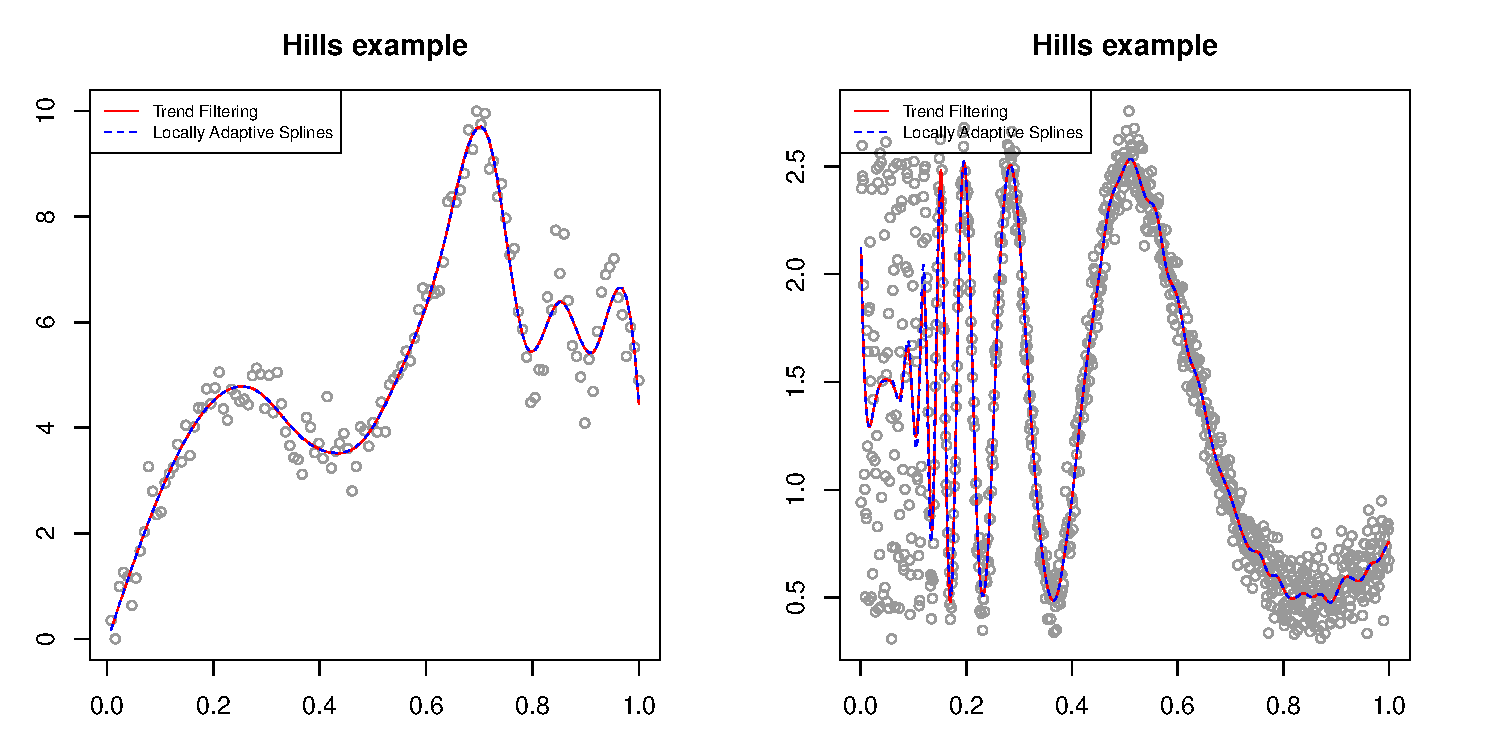
\includegraphics[width = 0.8\textwidth]{Figures/Figure7.pdf}
\caption{Comparison of cubic trend filtering and cubic locally adaptive spline with the same tuning parameter on the "hills" data and Doppler data. There is no visual difference in the "hills" data (left panel), and only tiny difference at $x= 0.1$ in the Doppler data (right panel). The difference between these two methods are only numerical.}
\label{fig:Figure7_lasvstf}
\end{figure}

In this subsection we empirically compare the estimates of trend filtering with locally adaptive spline. We revisit the two heterogeneous signals considered in Section \ref{subsec:sssimu} in Figure \ref{fig:Figure7_lasvstf}. Estimates of the two methods can be seen to be extremely similar. There is no visible difference for the "hills" data, and very tiny difference at $x = 0.1$ in the Doppler data. Even though we only show here the case for $k = 3$, such similarity exists for all orders in our simulation. We will prove in Section \ref{sec:theory} that asymptotically, the estimates of these two methods with the same tuning parameter converge to each other. However, their similarity in finite sample is beyond the explanation in this paper and is still an open question.

\subsection{Computational Comparison}
One way to solve the locally adaptive spline is to solve its Lasso form \eqref{eq:las_lasso} or its generalized Lasso form \eqref{eq:las_genlasso}. To make computation efficient, we need to choose an appropriate basis $(g_1,\ldots,g_n)$ so that the penalty matrix $C$ and design matrix $G$ are as sparse as possible. There is a dilemma here though. On one hand, the truncated power basis \eqref{eq:trun_basis} will make penalty $C$ identity but design $G$ dense. On the other hand, the B-spline basis with local support makes the design $G$ sparse but penalty $C$ dense. Therefore we are more of less stuck with a dense (generalized) Lasso problem.

\cite{mammen1997locally} proposed an alternative to solve the locally adaptive spline. For $k = 1$, the proposed algorithm solves \eqref{eq:las_constrained} for a given $\lambda$ in $\cal{O}(n\log(n))$ operations and $\cal{O}(n^2)$ operations for all $\lambda$. However, there is no guaranteed cost of the algorithm for $k\geq 2$ (the authors conjectured the algorithm takes also $\cal{O}(n^2)$ operations for all $\lambda$). We therefore conclude that locally adaptive spline is not as computationally efficient as trend filtering. 

\section{Real Data Study}
\label{sec:real_data}

\subsection{Serenoa NMR Data}
\label{subsec:nmr}

\begin{figure}[t!]
\centering
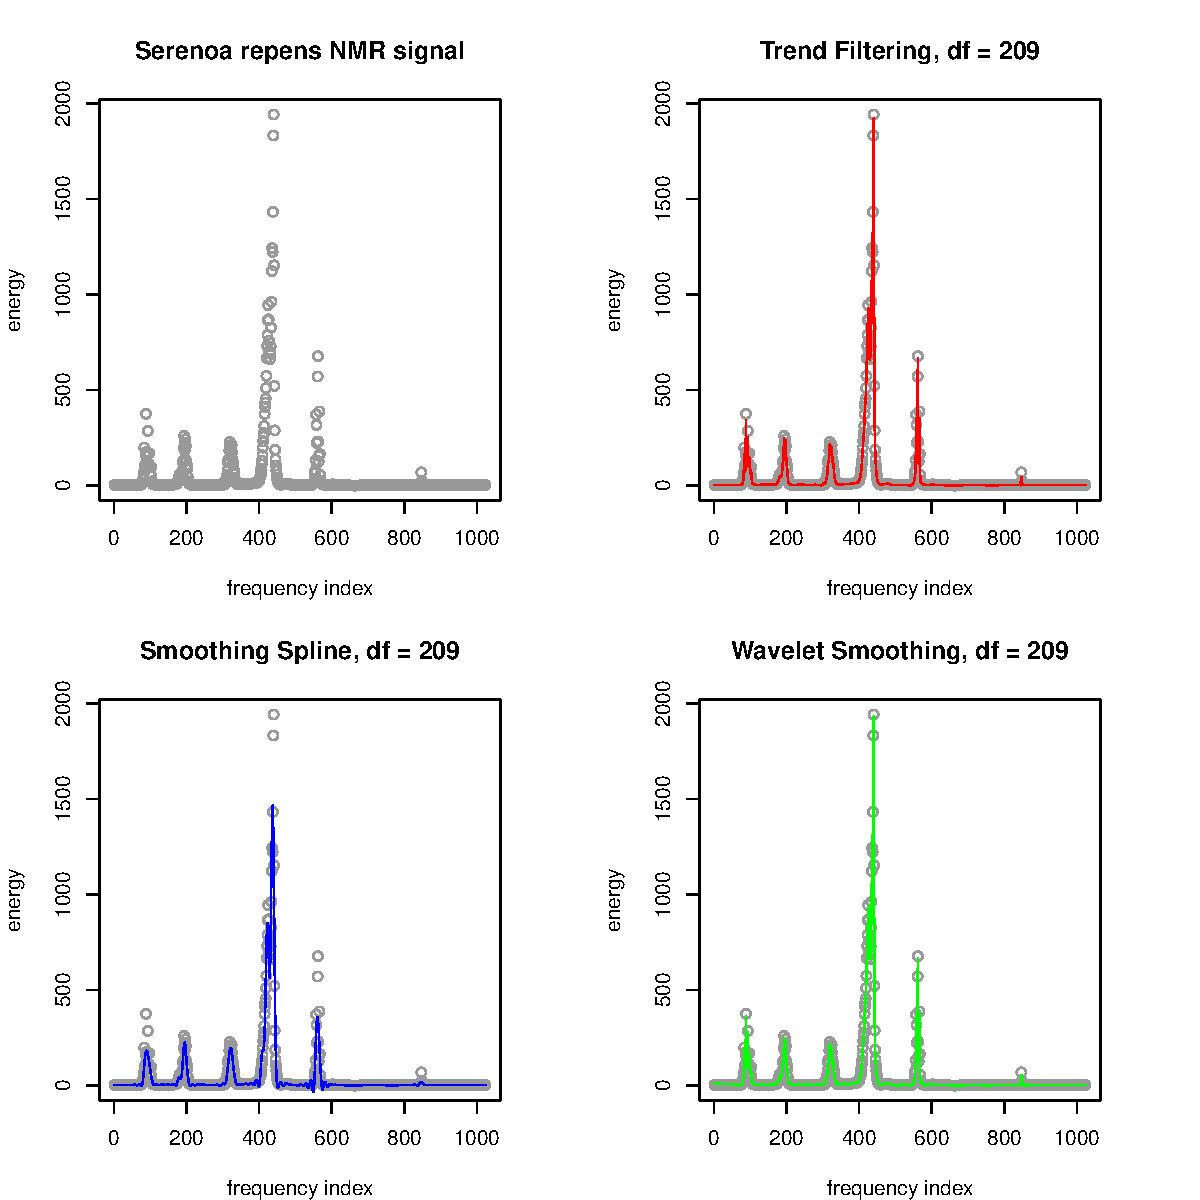
\includegraphics[width = 0.9\textwidth]{Figures/Figure9.pdf}
\caption{Top left panel: $n=1024$ measurements of frequency and energy in a NMR spectrum. Top right panel: estimate of cubic trend filtering with 209 degrees of freedom. Bottom left panel: smoothing spline with 209 degrees of freedom. Bottom right panel: wavelet smoother with 209 degrees of freedom. Smoothing spline suffers from over-smoothing at the spikes(especially the 1st, 4th and 5th one). Trend filtering and wavelet smoothing give very similar estimates and both perform very well on both the smooth part and the spikes. Close inspection shows that trend filtering does slightly better at the smooth part, as the wavelet estimate is a little wiggly at the transition between flats and spikes.}
\label{fig:Figure_9}
\end{figure}


In this subsection, we examine one of the Nuclear Magnetic Resonance (NMR) spectra data to compare the performance of different methods. The data is available at \url{https://github.com/bryanhanson/ChemoSpec}. This data contains a collection of 14 NMR spectra of essential oil extracted from the
palm \emph{Serenoa repens} or Saw Palmetto, which is commonly used to treat
benign prostatic hyperplasia (BPH) in men. The NMR uses the magnetic properties of atomic nuclei to get information about an oil sample. More specifically, it detects the amount of energy at 32,768 frequencies in the spectrum of the sample. Since most frequencies have nearly zero energy, we choose an informative segment of $n = 1024$ frequencies and corresponding energy count. The true measurement is shown in the top left panel of Figure \ref{fig:Figure_9}.

We compare the estimates of trend filtering, smoothing spline and wavelet smoothing. The estimate of locally adaptive spline is omitted here due to its extreme similarity to trend filtering, as shown in Section \ref{sec:las_compare}. The smoothing spline is implemented by the \textit{smooth.spline} function in R, and wavelet smoothing is implemented by the \textit{wavethresh} package in R. The "wavelets on the interval" option in the \textit{wd} function in the \textit{wavethresh} package is chosen to handle the boundary conditions (as periodicity and symmetry are not appropriate assumptions for the boundary behavior in this example), which uses the algorithm of Cohen, Daubechies and Vial\cite{cohen1993wavelets}. Note that wavelet smoothing usually requires the sample size $n$ to be a power of $2$, thus we choose our segment length as $1024$ to satisfy this requirement. We choose $df = 209$ for trend filtering pick up the spikes, we then calibrate the estimates of smoothing spline and wavelet using this same degrees of freedom.

The estimates of trend filtering, smoothing spline and wavelet smoothing are shown in the top right panel, bottom left panel and bottom right panel of Figure \ref{fig:Figure_9} respectively. Trend filtering clearly outperforms smoothing spline as smoothing spline severely over-smoothes the spikes, especially the 1st, 4th and 5th one. Wavelet smoothing gives very similar estimate to trend filtering, performing pretty well on both the smooth part and the spikes. Close inspection shows that trend filtering does slightly better at the smooth part, as the wavelet estimate is a little wiggly at the transition between flats and spikes.

\subsection{Bone Mineral Density Data}
\label{subsec:bone}

\begin{figure}[t!]
\centering
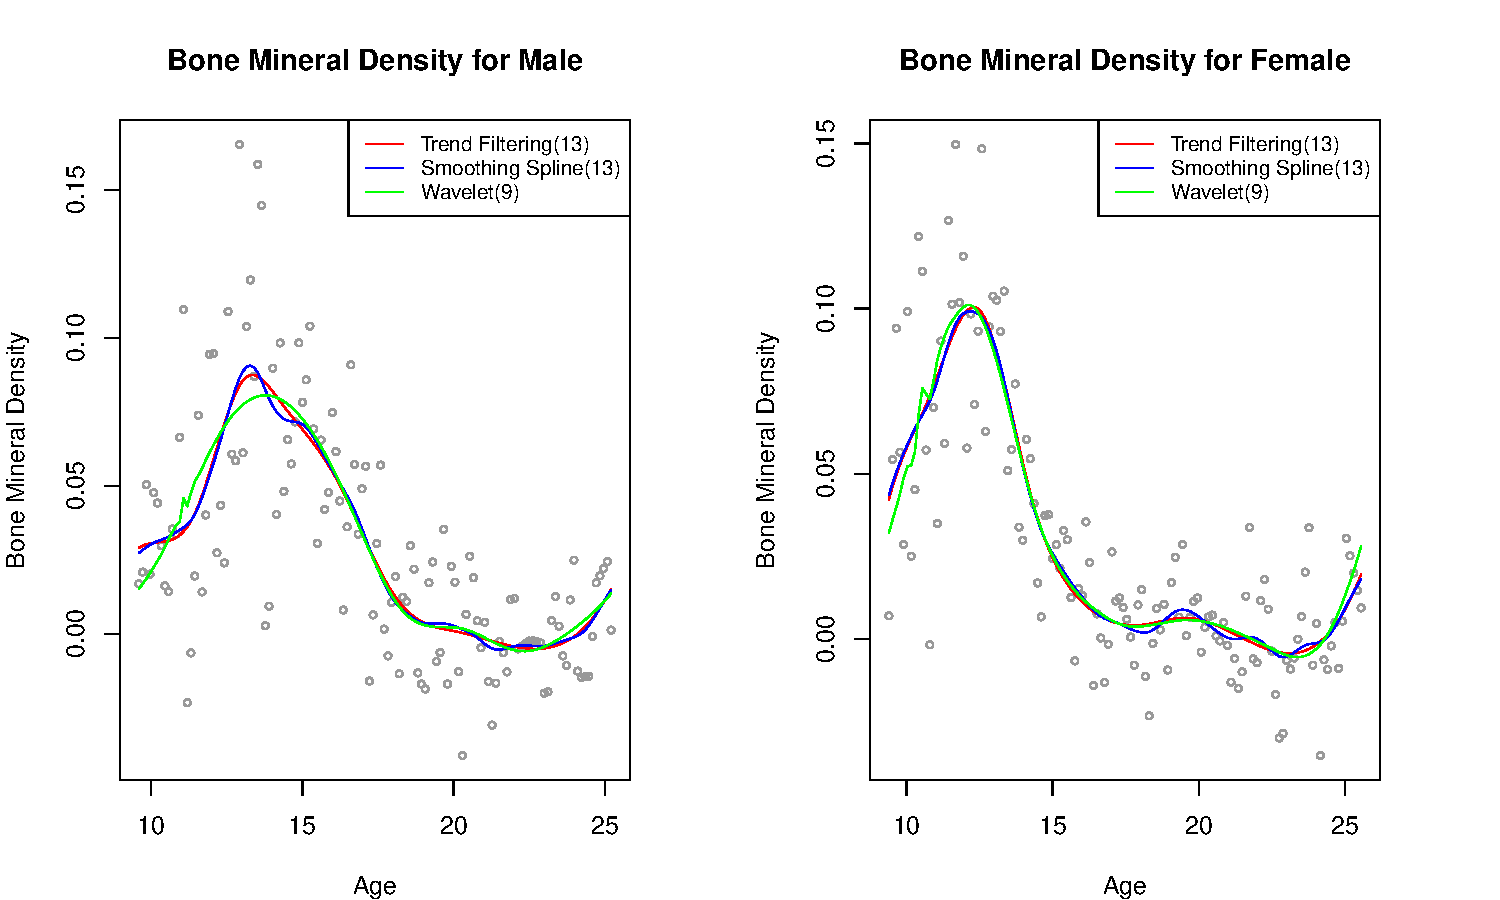
\includegraphics[width = 0.9\textwidth]{Figures/Figure9b.pdf}
\caption{Comparison of cubic trend filtering (red), cubic smoothing spline (blue) and wavelet smoother (green) on the bone mineral density data with 13, 13, 9 degrees of freedom respectively. Grey points are noisy observations, x axis marks the input variable "Age" and y axis marks the response variable "Bone Mineral Density". In both data sets for male and female, trend filtering has similar estimate to smoothing spline. Wavelet smoother, though using a smaller number of degrees of freedom, is a little jagged near the left boundary.}
\label{fig:real_bone}
\end{figure}
We have shown that trend filtering is locally adaptive when the true signal has heterogeneous levels of smoothness over the domain. Next we consider two cases with homogeneous smoothness and demonstrate that in such case trend filtering performs as well as linear smoothers such as smoothing spline. The first data set we consider measures the impact of age on the bone mineral density in males and females. Note this data set has been considered in Section 5.4 of \cite{friedman2001elements} and is available as \textit{bone} in the R package \textit{ElemStatLearn}. 

We compare the performance of cubic trend filtering, cubic smoothing spline and wavelet smoother on the bone density data for both male and female in Figure \ref{fig:real_bone}. Three methods are tuned to have $13, 13$ and $9$ degrees of freedom respectively. In both data sets, trend filtering has similar estimate to smoothing spline. Wavelet smoother, though using a smaller number of degrees of freedom, is a little wiggly near the left boundary.

\subsection{Ozone Data}
\label{subsec:real_ozone}

\begin{figure}[t!]
\centering
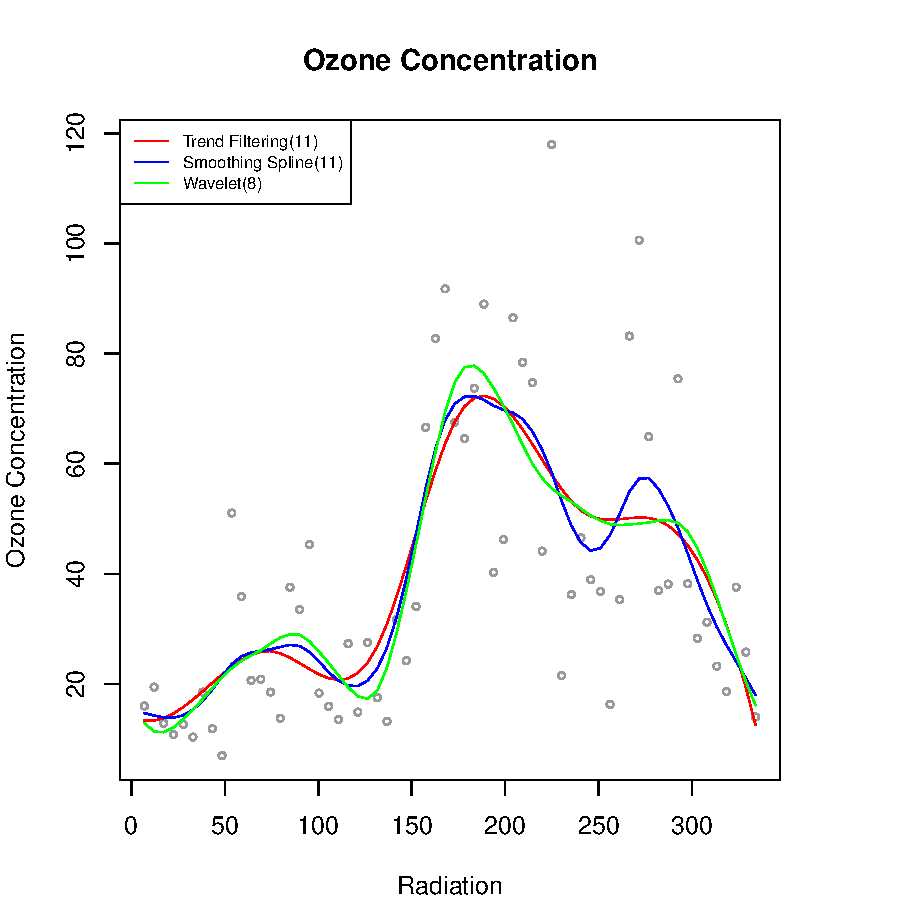
\includegraphics[width = 0.9\textwidth]{Figures/Figure9c.pdf}
\caption{Comparison of cubic trend filtering (red), cubic smoothing spline (blue) and wavelet smoother (green) on the ozone data with 13, 13 and 8 degrees of freedom respectively. Grey points are the sub-sampled $64$ noisy observations, x axis marks the amount of solar radiation and y axis marks the response ozone concentration. All three methods give similar estimate on the left half of the data, with smoothing spline showing an extra "hill" shape near the right boundary.}
\label{fig:real_ozone}
\end{figure}

Finally we consider another real data set \textit{ozone} from the \textit{ElemStatLearn} R package. This data set measures the relationship between ozone concentration and daily maximum temperature, solar radiation, wind speed for 111 days from May to September 1973 in New York. For our study, we focus on the marginal relationship between ozone concentration and solar radiation. Since wavelet smoother requires the sample size to be a power of $2$, we randomly sample $64$ out of $111$ measurements to satisfy this requirement. 

Again we compare the estimates of cubic trend filtering, cubic smoothing spline and wavelet smoother in Figure \ref{fig:real_ozone}. For this data set, all three methods give similar estimates for the left half of the domain, with smoothing spline showing a small "hill" shape near the right boundary.

\section{Convergence Rate}
\label{sec:theory}
In this section, we assume the same data model \eqref{eq:nonpara_model} with evenly-spaced inputs, i.e. $x_i = \frac{i}{n}$, $i = 1,\ldots, n$. Errors $\epsilon_i$ are assumed to be sub-Gaussian with mean zero, that is
\begin{align*}
\E(\epsilon_i) = 0 \quad \text{ and } \quad P(|\epsilon_i|\geq t) \leq M\mbox{exp}(-t^2/(2\sigma^2)) \quad \text{ for all } t>0, i=1,\ldots, n
\end{align*}
where $M, \sigma$ are some constants. We will write $A_n = \cal{O}_p(B_n)$ to denote that $A_n/B_n$ is bounded in probability, for random sequences $A_n,B_n$. We will also write $a_n = \Omega(b_n)$ to denote that $1/a_n = \cal{O}(1/b_n)$ for non-random sequences $a_n, b_n$, and finally $a_n = \Theta(b_n)$ to denote that $a_n = \cal{O}(b_n)$ and $a_n = \Omega(b_n)$.

\subsection{Minimax Convergence Rate}
\label{subsec:minimax_rate}
In nonparametric statistics, we usually have very little prior knowledge about the true function $f_0$ in \eqref{eq:nonpara_model}. So instead of assuming a specific form of the true function $f_0$, e.g. linear, piecewise polynomial, etc, we only assume that $f_0$ lies in some smooth function class $\cal{F}$. Correspondingly, when talking about consistency and convergence rate, instead of considering the parametric rate as in the parametric setting, we characterize the performance of an estimator in terms of the minimax rate, which, roughly speaking, is the best achievable convergence rate over the assumed function class $\cal{F}$. More rigorously, the minimax convergence rate over a function class $\cal{F}$ is defined as

\begin{align*}
\min_{\hat{f}}\max_{f_0\in\cal{F}} \mathbb{P}(L(\hat{f}, f_0))
\end{align*}
where the first minimization is taken over all possible estimators, and the second maximization is taken over all possible true function $f_0$ in $\cal{F}$. The $\mathbb{P}$ is the functional form for integral under measure $\mathbb{P}$, and $L(\cdot, \cdot)$ is the loss function. $\mathbb{P}(L(\hat{f}, f_0))$ is also called the risk under measure $P$ in some literature. The most frequently used loss function is the classical $L_2$ loss, and $\mathbb{P}$ is usually taken to be the $\mathbb{P}_x$, which is the true distribution of the input if assumed to be random, or $\mathbb{P}_n$, the empirical norm when the input $x$ is assumed to be fixed. For the rest of the section, we will adopt $L_2$ loss under the fixed-design setting, in which case the minimax rate becomes

\begin{align}
\min_{\hat{f}}\max_{f_0\in\cal{F}}\frac{1}{n}\sum_{i=1}^n(\hat{f}(x_i)-f_0(x_i))^2
\label{eq:minimax}
\end{align}
Clearly, when the inputs $(x_1,\ldots, x_n)$ are fixed, the minimax rate \eqref{eq:minimax} depends on the underlying function class $\cal{F}$. Some frequently used classes to characterize smoothness include: H\"older class, Sobolev class, total variation class, etc. The $k$th order Sobolev smoothness class with bound $C$ is defined to be 

\begin{align*}
\cal{W}_k(C) = \{f:[0, 1]\rightarrow \RR: f \text{ is $k$ times differentiable and } \int_0^1(f^{(k)}(t))^2dt\leq C\}
\end{align*}
and the $k$th order total variation class with bound $C$ is defined as

\begin{align*}
\cal{F}_k(C)=\{f:[0, 1]\rightarrow \RR: f \text{ is $k$ times weakly differentiable and TV($f^{(k)}$)$\leq C$}\}
\end{align*}
Minimax rate over the Sobolev classes are well-studied, and it is know (see e.g. \cite{nussbaum1985spline}) that
\begin{align*}
\min_{\hat{f}}\max_{f_0\in\cal{W}_k(C)} \E[\frac{1}{n}\sum_{i=1}^n(\hat{f}(x_i)-f_0(x_i))^2] = \Omega(n^{-2k/(2k+1)})
\end{align*}
By functional space embedding theory, $\cal{W}_{k+1}(C)\subset \cal{F}_k(C)$, thus it follows that
\begin{align*}
\min_{\hat{f}}\max_{f_0\in\cal{F}_k(C)}\E[\frac{1}{n}\sum_{i=1}^n(\hat{f}(x_i)-f_0(x_i))^2] = \Omega(n^{-(2k+2)/(2k+3)})
\end{align*}
Definition of the minimax convergence rate tells us that we can expect to do no better than $n^{-(2k+2)/(2k+3)}$. In other words, $n^{-(2k+2)/(2k+3)}$ is a lower-bound of the minimax rate over the class $\cal{F}_k(C)$. So a natural question is whether $n^{-(2k+2)/(2k+3)}$ is also the upper bound and does any method achieve this minimax rate. \cite{mammen1997locally} gives an affirmative answer to this question. Theorem 10 of \cite{mammen1997locally} proved that the $k$th order locally adaptive spline $\hat{f}$ corresponding to tuning parameter $\lambda=\Theta(n^{1/(2k+3)})$ satisfies

\begin{align*}
\frac{1}{n}\sum_{i=1}^n (\hat{f}(x_i)-f_0(x_i))^2 = \cal{O}_p(n^{-(2k+2)/(2k+3)})
\end{align*}
and also that $TV(\hat{f}) = \cal{O}_p(1)$. In words, this tells us that the minimax rate over $\cal{F}_k(C)$ is indeed $\cal{O}_p(n^{-(2k+2)/(2k+3)})$ and locally adaptive spline is optimal in the minimax sense. 

On the other hand, \cite{donoho1998minimax} proves that any linear smoother, i.e. estimate linear in $y$ is sub-optimal in the minimax sense over $\cal{F}_k(C)$. Using functional space embedding theory and minimax bounds on the Besov space this time, \cite{donoho1998minimax} proves the following lower bound for linear smoother
\begin{align*}
\min_{\hat{f}\text{ linear}}\max_{f_0\in\cal{F}_k(C)} \E[\frac{1}{n}\sum_{i=1}^n (\hat{f}(x_i) - f_0(x_i))^2] = \Omega(n^{-(2k+1)/(2k+2)})
\end{align*}
In other words, any linear smoother can be expected to do no better than $n^{-(2k+1)/(2k+2)}$ over $\cal{F}_k(C)$, which is sub-optimal. This implies, as a special case, that smoothing spline is sub-optimal in the minimax sense. See Figure \ref{fig:diagram} for a graphical illustration of minimax optimality.

\subsection{Convergence Rate of Trend Filtering: Bounded Total Variation}
In this subsection, we show that our method, trend filtering, is also minimax optimal over the bounded total variation class $\cal{F}_k(C)$. The idea of the proof is simple: we prove that the estimate of trend filtering converge to the estimate of locally adaptive spline in the minimax rate and then apply the result that locally adaptive spline is minimax optimal. This is formalized in the following theorem and corollary. The proof is deferred to the supplement. 
\begin{theorem}
Assume that $y\in\RR^n$ is drawn from the model \eqref{eq:nonpara_model}, with evenly-spaced inputs $x_i = i/n$, $i = 1,\ldots, n$ and i.i.d. sub-Gaussian errors. Assume also that $f_0\in\cal{F}_k(C)$, that is, for a fixed integer $k\geq 0$ and constant $C > 0$, the true function $f_0$ is $k$ times weakly differentiable and $TV(f_0^{(k)})\leq C$. Let $\hat{f}$ denote the $k$th order locally adaptive spline estimate defined in \eqref{eq:las_constrained} with tuning parameter $\lambda = \Theta(n^{1/(2k+3)})$, and let $\hat{u}$ be the $k$th order trend filtering estimate defined in \eqref{eq:tf} with tuning parameter $(1+\delta)\lambda$, for any fixed $\delta > 0$. Then 
\begin{align}
\frac{1}{n}\sum_{i=1}^n(\hat{u}_i - \hat{f}(x_i))^2 = \cal{O}_p(n^{-(2k+2)/(2k+3)})
\label{eq:tflas}
\end{align}
\label{thm:1}
\end{theorem}
Note that the convergence rate of trend filtering and locally adaptive spline on the right-hand side of \eqref{eq:tflas} is the minimax rate over the class $\cal{F}_k(C)$. This, when combined with the fact that locally adaptive spline is minimax optimal, gives the following corollary immediately.

\begin{corollary}
Under the assumptions of Theorem \ref{thm:1}, for a tuning parameter $\lambda = \Theta(n^{1/(2k+3)})$, the $k$th order trend filtering estimate $\hat{u}$ defined in \eqref{eq:tf} satisfies
\begin{align*}
\frac{1}{n}\sum_{i=1}^n (\hat{u}_i - f_0(x_i))^2 = \cal{O}_p(n^{-(2k+2)/(2k+3)})
\end{align*}
\end{corollary}
This concludes the claim that trend filtering is minimax optimal over the function class $\cal{F}_k(C)$.

\subsection{Convergence Rate of Trend Filtering: Growing Total Variation}
In this subsection, we consider the convergence rate of trend filtering over function class with growing total variation. This will encompass the previous subsection as a special case. The idea, however, is still the same. We rely on the result from \cite{mammen1997locally} and prove that the estimates of trend filtering and locally adaptive spline are asymptotically very close.

\begin{theorem}
Assume that $y\in\RR^n$ is drawn from the model \eqref{eq:nonpara_model}, with inputs $x_i = i/n$, $i=1,\ldots, n$ and i.i.d. sub-Gaussian errors. Also assume that $f_0\in\cal{F}_k(C_n)$, that is, for a fixed integer $k\geq 0$ and $C_n > 0$ (depending on $n$), the true function $f_0$ is $k$ times weakly differentiable and $TV(f^{(k)}_0)\leq C_n$. Let $\hat{f}$ denote the $k$th order locally adaptive spline estimate defined in \eqref{eq:las_constrained} with tuning parameter $\lambda = \Theta(n^{1/(2k+3)}C_n^{-(2k+1)/(2k+3)})$, and let $\hat{u}$ denote the $k$th order trend filtering estimate in \eqref{eq:tf} with tuning parameter $(1+\delta)\lambda$, for any fixed $\delta >0$. If $C_n$ does not grow too quickly, that is

\begin{align}
C_n = \cal{O}(n^{1/(2k+2)})
\label{eq:tv_rate}
\end{align}
then
\begin{align*}
\frac{1}{n}\sum_{i=1}^n(\hat{u}_i - \hat{f}(x_i))^2 = \cal{O}_p(n^{-(2k+2)/(2k+3)}C_n^{2/(2k+3)})
\end{align*}
\label{thm:2}
\end{theorem}

Again by combining with the triangular inequality, Theorem \ref{thm:2} implies the following corollary.

\begin{corollary}
Under the assumptions of Theorem \ref{thm:2}, for $C_n = \cal{O}(n^{1/(2k+2)})$ and a tuning parameter value $\lambda = \Theta(n^{1/(2k+3)}C_n^{2/(2k+3)})$, the $k$th order trend filtering estimate $\hat{u}$ defined in \eqref{eq:tf} satisfies
\begin{align*}
\frac{1}{n}\sum_{i=1}^n(\hat{u}_i - f_0(x_i))^2 = \cal{O}_p(n^{-(2k+2)/(2k+3)}C_n^{2/(2k+3)})
\end{align*}
\label{cor:2}
\end{corollary}

Theorem \ref{thm:2} and Corollary \ref{cor:2} demonstrate that for underlying function with growing total variation, the estimate of trend filtering has the same convergence rate as locally adaptive spline under the extra assumption that $C_n$ grows no faster than $\cal{O}(n^{1/(2k+2)})$. However, note that this assumption is not necessary for $k = 0, 1$ because for these two orders, the estimates of trend filtering and locally adaptive spline are the same by Lemma \ref{lemma:lasequivtf}.

\section{Extension and Discussion}
\label{sec:extension}
In this section, we consider several extensions of trend filtering. We also discuss the generalization of trend filtering to unevenly-spaced inputs. 

\subsection{Multivariate Trend Filtering}
The original definition of trend filtering \eqref{eq:tf} only applies in the univariate case, thus a natural extension to higher dimensions is multivariate trend filtering. There are generally two paths to higher dimensions. The first path is "truly" multivariate by constructing an appropriate multivariate discrete difference operator as the $D^{(k)}$ in \eqref{eq:tf}. Similar strategy has been taken for smoothing spline, where univariate natural cubic spline is extended to thin plate splines\cite{green1993nonparametric,wahba1990spline}. The analogous approach for trend filtering is an open question and a topic of individual interest.

The other more modest approach is to fit an additive model with trend filtering estimate in each dimension. The general additive model\cite{hastie1990generalized} has the following form

\begin{align}
y_i = \sum_{j=1}^pf_j(x_{ij}) + \epsilon_i, \qquad i=1,\ldots, n
\label{eq:additive}
\end{align}
where each $x_i=(x_{i1},\ldots, x_{ip})$ is $p$-dimensional input, $f_j$ is the true regression function for each dimension, thus \eqref{eq:additive} doesn't consider interaction between covariates. Generally, any univariate smoother can be plugged in to estimate each $f_j$. Given the superior performance of trend filtering in the univariate setting, it's worth considering adopting trend filtering to estimate each $f_j$ and then compare with additive models built from other univariate smoothers, e.g. smoothing spline, wavelets, etc.

\subsection{Synthesis versus Analysis}
\label{subsec:syn_vs_ana}
Synthesis approach and analysis approach are two terminologies from signal processing. Given a noisy observation and the goal to recover the true underlying signal, the synthesis approach builds the estimate via a linear combination of a set of basis, or in some literature, "atoms"; and the analysis approach directly estimates the true signal by penalizing the undesired structure in the estimate. In the context of $\ell_1$ penalized estimation, these two approaches consider the following two problems respectively:

\begin{align}
\hat{\theta} &\in \argmin_{\theta\in\RR^p}\frac{1}{2}\|y-X\theta\|_2^2 + \lambda\|\theta\|_1
\label{eq:synthesis}
\end{align}
\begin{align}
\hat{\beta} &\in \argmax_{\beta\in\RR^n}\frac{1}{2}\|y-\beta\|_2^2 + \lambda\|D\beta\|_1
\label{eq:analysis}
\end{align}
where $y\in\RR^n$ is the observed noisy signal. The synthesis approach \eqref{eq:synthesis} estimates the linear coefficient $\hat{\theta}$ of the basis, which in this case is the set of columns of $X$, and then estimate the true signal by $\hat{y} = X\hat{\theta}$. On the contrary, in the analysis framework \eqref{eq:analysis}, the estimate $\hat{y} = \hat{\beta}$ and the penalty is on the undesired structure characterized by $D$.

The synthetic approach and analysis approach can be seen as two angles of a problem and are equivalent in certain cases. In trend filtering, for example, the original definition \eqref{eq:tf} lies in the analysis framework while its equivalent Lasso form representation \eqref{eq:tf_lasso} lies in the synthetic framework. There is no universal better choice between these two approaches, but it turns out the analysis framework is more flexible to extend the trend filtering estimate by mixing penalties.

\begin{figure}[t!]
\centering
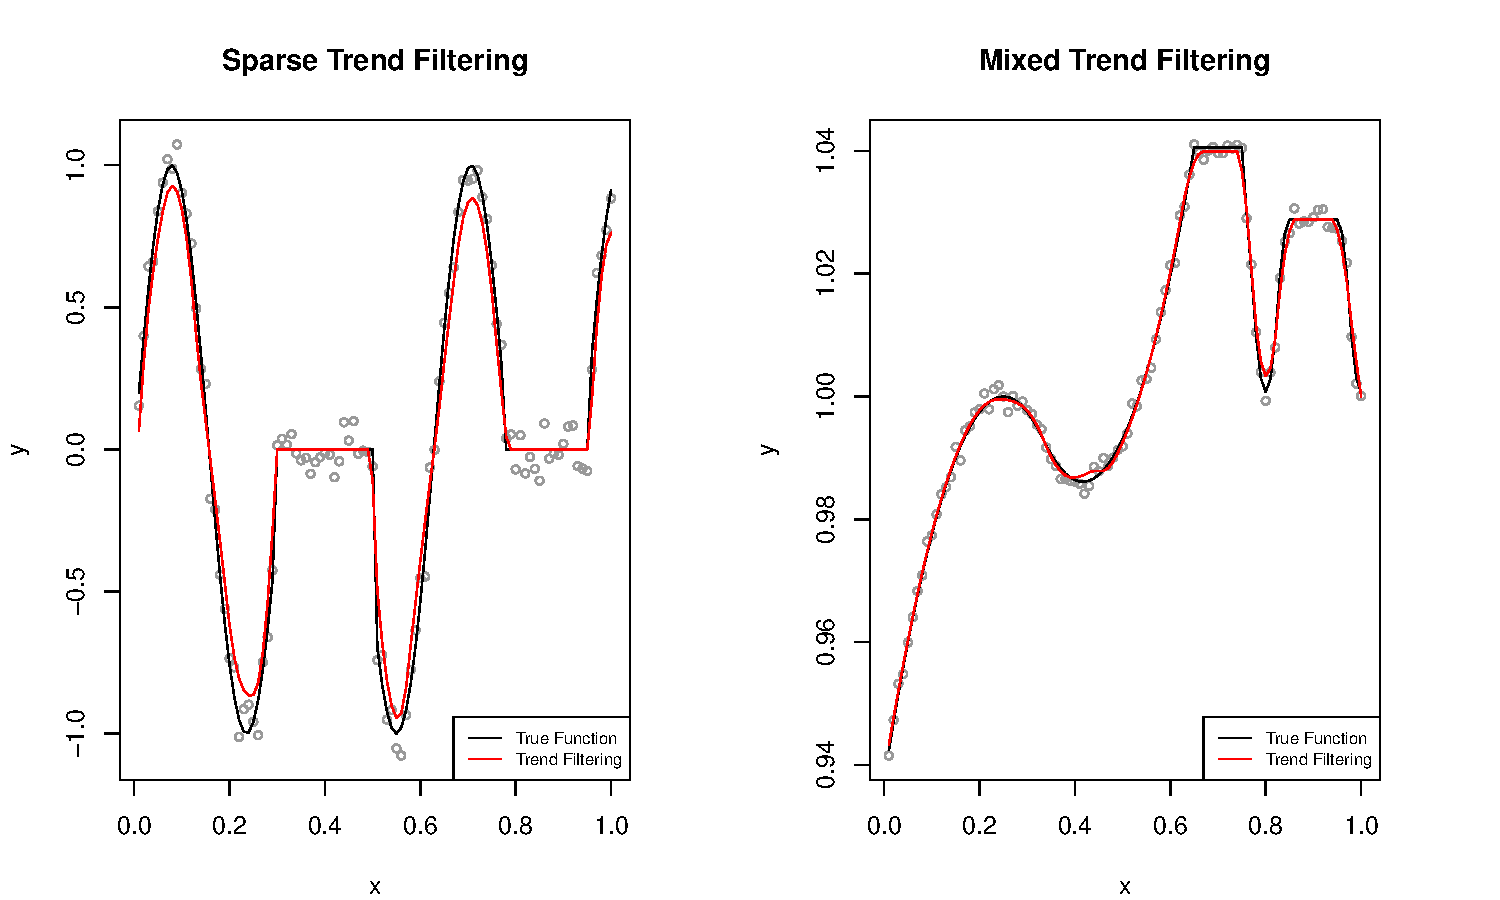
\includegraphics[width = 0.9\textwidth]{Figures/Figure11.pdf}
\caption{Extensions of trend filtering: sparse trend filtering (left panel) and mixed trend filtering (right panel). In the left panel, we fit sparse trend filtering estimate with $k = 2$, the extra $\ell_1$ penalty on the estimate leads to two zero-valued segments. In the right panel, we fit mixed trend filtering with $k=0,2$, this leads to a combination of piecewise quadratic and piecewise constant structure.}
\label{fig:sparse_mixed_tf}
\end{figure}

The first extension is a sparse version of trend filtering. Suppose we want to fit a cubic trend filtering model but prefer the estimate to be exactly zero for certain segments of the domain, then it is appealing to consider the following problem:

\begin{align}
\hat{u} = \argmin_{u\in\RR^n}\frac{1}{2}\|y-u\|_2^2 + \lambda_1\|D^{(k+1)}u\|_1 + \lambda_2\|u\|_1
\label{eq:sparse_tf}
\end{align}
where we mix the structural penalty $\|Du\|_1$ as in \eqref{eq:tf} and the new sparsity penalty $\|u\|_1$ directly applied to the estimate. We call \eqref{eq:sparse_tf} sparse trend filtering. A possible application of \eqref{eq:sparse_tf} is to model the difference between two co-evolving time series, where in certain time segments the two series are believed to share the same value. In the left panel of Figure \ref{eq:sparse_tf}, we fit a quadratic sparse trend filtering ($k=2$), the extra $\ell_1$ penalty directly applied to the estimate leads to two zero-valued segments in the estimate. 

Another example is trend filtering with varying order of smoothness. In certain cases, prior knowledge may indicate that the true signal has different level of smoothness in different segments of the domain, e.g. piecewise constant in certain parts and piecewise cubic in others. In such case, it is desirable to consider the following trend filtering with mixed orders:

\begin{align}
\hat{u} \in \argmin_{u\in\RR^n}\frac{1}{2}\|y-u\|_2^2 + \lambda_1\|D^{(k_1+1)}u\|_1 + \lambda_2\|D^{(k_2+1)}u\|_1
\label{eq:mix_tf}
\end{align}
where we mix the $(k_1+1)$st and $(k_2+1)$st order discrete differences. One might expect the estimate of \eqref{eq:mix_tf} to display a mixed structure of piecewise polynomials. The fit of mixed trend filtering with $k=0,2$ in the right panel of Figure \ref{fig:sparse_mixed_tf} verifies this claim. 

For computational purpose, notice that both \eqref{eq:sparse_tf} and \eqref{eq:mix_tf} are equivalently generalized Lasso problem with two sub-blocks of penalty matrices stacked by row. Thus they can be solved by general path algorithms such as \cite{tibshirani2011solution,arnold2016efficient}; a specialized yet more efficient algorithm to solve generalized Lasso with identity design is recently proposed in \cite{ramdas2016fast}.

\subsection{Trend Filtering for Unevenly-Spaced Inputs}
\label{subsec:uneven}
Up to now, we have made the assumption that the inputs $(x_1,\ldots, x_n)$ are evenly-spaced. This is clearly not a reasonable assumption in real application, our goal in this subsection is to extend trend filtering to unevenly-spaced inputs. Recall the line of thinking to deal with evenly-spaced trend filtering is to first define the discrete difference operator in \eqref{eq:tf}, invert it to obtain the equivalent Lasso form \eqref{eq:tf_lasso}, and finally use the falling factorial basis to propose a continuous version of trend filtering \eqref{eq:fall_fact}. For trend filtering with unevenly-spaced inputs, we reverse this thinking. We start with the continuous version of trend filtering via the falling factorial basis \eqref{eq:fall_fact}, which when evaluated at the unevenly-spaced inputs $(x_1,\ldots, x_n)$ outputs a design matrix $H^{(x)}$, where the superscript is to indicate the dependence on the inputs. Next we invert the design matrix to transform the Lasso problem back to a generalized Lasso problem. More accurately, denote the new version of discrete difference operator as $D^{(x,k+1)}$, where again the superscript is used to indicate the dependence on input and the order. We look for $D^{(x,k+1)}$ such that

\begin{align*}
\hat{\alpha} = \argmin_{\alpha\in\RR^n} \frac{1}{2}\|y-H^{(x)}\|_2^2 + \lambda\sum_{j=k+2}^b|\alpha_j|
\end{align*}
and 
\begin{align*}
\hat{u} = \argmin_{u\in\RR^n} \frac{1}{2}\|y-u\|_2^2 + \frac{1}{k!}\cdot\lambda\|D^{(x,k+1)}u\|_1
\end{align*}
satisfy the requirement $\hat{u} = H^{(x)}\hat{\alpha}$. Simple matrix inversion shows that $D^{(x,k+1)}$ is the last $n-k-1$ row of $(H^{(x)}/k!)^{-1}$. More explicitly, when $k = 0$, $D^{(x,1)} = D^{(1)}$, the first order discrete difference operator defined in \eqref{eq:D_0}. Then through induction, we can show that

\begin{align}
D^{(x,k+1)} = D^{(1)} \cdot \mbox{diag}(\frac{k}{x_{k+1}-x_1}, \frac{k}{x_{k+2} - x_2}, \ldots, \frac{k}{x_n-x_{n-k}}) \cdot D^{(x,k)}
\label{eq:D_uneven}
\end{align}
where $D^{(1)}$ is the $(n-k-1) \times (n-k)$ version of the first order difference matrix. This newly defined $D^{(x, k+1)}$ can still be thought of as a discrete analogue of derivative, but adjusted to account for unevenly spaced inputs.

Next we discuss how this generalization to unevenly-spaced inputs affects the computational and theoretical properties of trend filtering. Fortunately, this generalization doesn't incur any extra cost for computation by noticing that the diagonal matrix in \eqref{eq:D_uneven} will not affect the banded structure of the difference operator. In other words, efficient algorithms such as the primal-dual interior point algorithm in \cite{kim2009ell_1} and the path algorithm for generalized Lasso such as \cite{harchaoui2010multiple,tibshirani2011solution} still apply. Note, however, that if the inputs $(x_1,\ldots, x_n)$ are highly irregular, i.e. some pairs of inputs have large distances while some others are very close to each other, this will lead to both very large and very small entries in $D^{(x,k+1)}$, which is likely to make algorithms numerically unstable. From a theoretical point, the previous "piggyback" approach with locally adaptive spline can still be used, but two extra assumptions need to hold: 

\begin{itemize}
\item Locally adaptive spline needs an extra assumption that the input points $(x_1,\ldots, x_n)$ will not be too far away from each other to maintain minimax properties, thus such assumption is also inherited by trend filtering. This is reflected by \eqref{eq:uneven_cond1} in the following theorem.
\item Recall that the key to link trend filtering and locally adaptive spline is the fact that the design matrices in their respective Lasso form are very close element-wise. This is still required in the case of unevenly-spaced inputs and is reflected by \eqref{eq:uneven_cond2} in the following theorem.
\end{itemize}

\begin{theorem}
Assume that $y\in\RR^n$ in drawn from the model \eqref{eq:nonpara_model}, with inputs $x_1<x_2<\ldots<x_n\in[0,1]$ and sub-Gaussian errors. Assume also that $f_0\in\cal{F}_k(C_n)$, i.e. for a fixed integer $k\geq 0$ and $C_n\geq 0$ (depending on $n$), the true function $f_0$ is $k$ times weakly differentiable and $TV(f_0^{k})\leq C_n$. Let $\hat{f}$ denote the $k$th order locally adaptive spline estimate defined in \eqref{eq:las_constrained} with tuning parameter $\lambda = \Theta(n^{1/(2k+3)}C_n^{-(2k+1)/(2k+3)})$, and let $\hat{u}$ denote the $k$th order trend filtering estimate in \eqref{eq:tf} with tuning parameter $(1+\delta)\lambda$, for any fixed $\delta >0$. Finally, if $k\geq 2$, then we must assume that the following conditions are met: $C_n$ does not grow too quickly,

\begin{align*}
C_n = O(n^{1/(2k+2)}),
\end{align*}
and the inputs $(x_1,\ldots, x_n)$ satisfy
\begin{align}
\max_{i=1,\ldots, n-1} (x_{i+1}-x+i) = O(n^{-(k+1)/k(2k+3)}C_n^{-(2k+2)/(k(2k+3))})
\label{eq:uneven_cond1}
\end{align}
and
\begin{align}
\max_{i=1,\ldots,n-k-1} |\prod_{i=1}^k(x_n-x_{i+l}) - (x_n-x_{i+\floor{(k+2)/2}})^k| = O(\frac{1}{n})
\label{eq:uneven_cond2}
\end{align}

Then 
\begin{align*}
\frac{1}{n}\sum_{i=1}^n (\hat{u}_i - \hat{f}(x_i))^2 = O_p(n^{-(2k+2)/(2k+3)}C_n^{2/(2k+3)})
\end{align*}
and furthermore
\begin{align*}
\frac{1}{n}\sum_{i=1}^n (\hat{u}_i-f_0(x_i))^2 = O_p(n^{-(2k+2)/(2k+3)}C_n^{2/(2k+3)})
\end{align*}
Hence, if the $k$th derivative of $f_0$ has bounded total variation, i.e. $C_n$ is a constant, then the trend filtering estimate converges to $f_0$ at minimax rate $n^{-(2k+2)/(2k+3)}$.
\label{thm:3}
\end{theorem}

As discussed before, \eqref{eq:uneven_cond1} is needed for the convergence rate of locally adaptive spline in \cite{mammen1997locally}, and thus inherited by trend filtering. The second condition \eqref{eq:uneven_cond2} is sufficient to imply
\begin{align*}
\|G_2^{(x)} - H_2^{(x)}\|_\infty = O(\frac{1}{n})
\end{align*}
where $G_2^{(x)}$ and $H_2^{(x)}$ are the last $n-k-1$ columns of the new design matrices $G^{(x)}$ and $H^{(x)}$ for unevenly-spaced inputs. Theorem \ref{thm:3} can be proved in a similar fashion to Theorem \ref{thm:2}.

\section{Conclusion}
\label{sec:conclusion}
We have shown that trend filtering, a newly proposed method for nonparametric estimation, is both fast and locally adaptive. Though the original definition is discrete in nature, we have proposed a continuous representation of trend filtering and shown that the estimate is piecewise polynomial. Empirically, we show that trend filtering adapts better to varying levels of smoothness than smoothing spline, and further, exhibits a remarkable similarity to locally adaptive spline. We have also theoretically justified trend filtering by proving that the estimate of trend filtering converges to the true function with minimax rate over true functions whose $k$th derivative has bounded total variation.

\bibliography{paperreview}

\appendix
\section*{Appendix}
\addcontentsline{toc}{section}{Appendices}
\renewcommand{\thesubsection}{\Alph{subsection}}
This appendix contains supplementary materials for the main body of the paper. Prefix "TF" will be used to refer to lemmas and theorems in the main body.

\subsection{Lasso and continuous representation of trend filtering}
\subsubsection{Proof of TF-Lemma 1}
\begin{proof}
The proof of this lemma basically inverts the $(k+1)$st order discrete difference operator $D^{(k+1)}$. Since $D^{(k+1)}$ is of dimension $\RR^{n-(k+1)\times n}$, thus we first "complete" the matrix by adding linearly independent rows. In words, let $\alpha = n^k/k!\cdot Du$ with $D\in\RR^{n\times n}$ defined as

\begin{align*}
D = 
\begin{bmatrix}
D^{(0)}_1\\
D^{(1)}_1\\
\vdots\\
D^{(k)}_1\\
D^{(k+1)}
\end{bmatrix}
\end{align*}
where $D^{(i)}_i\in\RR^n$ denotes the first row of the $i$th discrete difference operator $D^{(i)}$ for $i = 0,1,\ldots, k$ (and $D^{(0)} = \mathbb{I}_n$ by convention). We first show that $D^{-1} = M$, where $M = M^{(0)}\cdot\ldots\cdot M^{(k)}$, and 

\begin{align*}
M^{(i)} = 
\begin{bmatrix}
\mathbb{I}_{i\times i} & 0\\
0 & L_{(n-i)\times(n-i)}
\end{bmatrix}
\text{ for } i = 0, \ldots, k
\end{align*}
Here $\mathbb{I}_{i\times i}$ is the identity matrix of dimension $i$, and $L_{(n-i)\times(n-i)}$ is the $(n-i)\times(n-i)$ lower triangular matrix of $1$s. We now prove $M^{-1} = D$ by induction. For $k = 0$, this can be easily seen by

\begin{align*}
\begin{bmatrix}
1 & 0 & 0 & \ldots & 0\\
1 & 1 & 0 & \ldots & 0\\
1 & 1 & 1 & \ldots & 0\\
\vdots\\
1 & 1 & 1 & \ldots & 1
\end{bmatrix}^{-1}
=
\begin{bmatrix}
1 & 0 & 0 & \ldots & 0 & 0\\
-1 & 1 & 0 & \ldots & 0 & 0\\
0 & -1 & 1 & \ldots & 0 & 0\\
\vdots\\
0 & 0 & 0 & \ldots & -1 & 1
\end{bmatrix}
\end{align*}
Assume now that the statement holds for $k -1$, then

\begin{align*}
(M^{(0)} \cdot \ldots \cdot M^{(k)})^{-1} &= (M^{(k)})^{-1} (M^{(0)\cdot\ldots\cdot M^{(k-1)}})^{-1}\\
&= 
\begin{bmatrix}
\mathbb{I}_k & 0\\
0 & L^{-1}_{(n-k)\times (n-k)}
\end{bmatrix}
\begin{bmatrix}
D_1^{(0)}\\
\vdots\\
D_1^{(k-1)}\\
D^{(k)}
\end{bmatrix}\\
&= 
\begin{bmatrix}
D_1^{(0)}\\
\vdots\\
D_1^{(k-1)}\\
L^{-1}D^{(k)}
\end{bmatrix}
\end{align*}
where in the second equality we use the inductive hypothesis. Moreover, 

\begin{align*}
L^{-1}D^{(k)} = 
\begin{bmatrix}
1 & 0 & 0 & \ldots & 0 & 0\\
-1 & 1 & 0 & \ldots & 0 & 0\\
0 & -1 & 1 & \ldots & 0 & 0\\
\vdots\\
0 & 0 & 0 & \ldots & -1 & 1
\end{bmatrix}
D^{(k)} = 
\begin{bmatrix}
D_1^{(k)}\\
D^{(k+1)}
\end{bmatrix}
\end{align*}
This completes the inductive proof. Therefore, substituting $\alpha = n^k/k!\cdot Du$ yields the problem
\begin{align*}
\hat{\alpha} = \argmin_{\alpha\in\RR^n} \frac{1}{2}\|y-\frac{k!}{n^k}M\alpha\|_2^2 + \lambda\sum_{j=k+2}^n|\alpha_j|
\end{align*}

It is now straightforward to check that the last $n-k-1$ columns of $(k!/n^k)M$ match those of $H$. Furthermore, the first $k+1$ columns of $(k!/n^k)M$ have the same linear span as the first $k+1$ columns of $H$, which is sufficient because the $\ell_1$ penalty only applies to the last $m-k-1$ coefficients. 
\end{proof}

\subsubsection{Proof of TF-Lemma 2}
\begin{proof}
Define $s_i^{(0)} = 1$ for all $i$, and 
\begin{align*}
s_i^{(k)} = \sum_{j=1}^{i-1}s_j^{(k-1)} \text{ for } k = 1,\ldots, 
\end{align*}
i.e. $s_i^{(k)}$ is the $k$th order cumulative sum of $(1,\ldots, 1)\in\RR^i$, with lag $1$. We will prove that
\begin{align}
\frac{(x-k)(x-k+1)\cdot\ldots\cdot (x-1)}{k!} = s_x^{(k)} \text{ for all } x = 1,\ldots \text{ and } k = 1,\ldots
\label{eq:cum_fall}
\end{align}
by induction on $k$. Note that this would be sufficient to prove the result in the lemma, as it would show that the bottom right $(n-k-1)\times (n-k-1)$ sub-block of $H$ in TF-\eqref{eq:H_cumsum}, which can be expressed as

\begin{align*}
\frac{k!}{n^k}\cdot
\begin{bmatrix}
s_{k+1}^{(k)} & 0 & \ldots & 0\\
s_{k+2}^{(k)} & s_{k+1}^{(k)} & \ldots & 0\\
\vdots\\
s_{n-1}^{(k)} & s_{n-2}^{(k)} & \ldots & s_{k+1}^{(k)}
\end{bmatrix}
\end{align*}
and coincides with the evaluations of the falling factorial basis \eqref{eq:fall_fact}. We now give inductive argument for \eqref{eq:cum_fall}. As for the base case, $k = 1$, clearly $x - 1=s_x^{(1)}$ for all $x$. Assume that the inductive hypothesis holds for $k$, then for any $x$,

\begin{align*}
s_x^{(k+1)} &= \sum_{i=1}^{x-1}\frac{(i-k)(i-k+1)\cdot\ldots\cdot(i-1)}{k!}\\
&= \sum_{i=1}^{x-1}\sum_{j=1}^{i-1}\frac{(j-k+1)(j-k+2)\cdot\ldots\cdot(j-1)}{(k-1)!}
\end{align*}
by the inductive hypothesis. Switching the order of the summations, 

\begin{align*}
s_x^{(k+1)} &= \sum_{j=1}^{x-2}\sum_{i=j+1}^{x-1}\frac{(j-k+1)(j-k+2)\cdot\ldots\cdot(j-1)}{(k-1)!}\\
&= \sum_{j=1}^{x-2} \frac{(j-k+1)(j-k+2)\cdot\ldots\cdot(j-1)}{(k-1)!}\cdot(x-j-1)\\
&= \sum_{j=1}^{x-2}\frac{(j-k+1)(j-k+2)\cdot\ldots\cdot(j-1)}{(k-1)!}\cdot(x-k-1-j+k)
\end{align*}
Grouping terms and again applying the inductive hypothesis,
\begin{align*}
s_x^{(k+1)} &= \frac{(x-k-1)(x-k-2)\cdot\ldots\cdot(x-2)}{k!}\cdot(x-k-1)-s_{x-1}^{(k+1)}\cdot k
\end{align*}
Noting that $s_x^{(k+1)} = s_{x-1}^{(k+1)}+(x-k-1)\cdot\ldots\cdot(x-2)/k!$, and rearranging terms gives
\begin{align*}
s_{x-1}^{(k+1)} = \frac{(x-k-2)(x-k-1)\cdot\ldots\cdot(x-2)}{(k+1)!}
\end{align*}
Since $x$ was arbitrary, this completes the inductive step, and hence the proof.
\end{proof}

\subsubsection{Proof of TF-Lemma 3}
\begin{proof}
This lemma is a trivial combination of TF-Lemma \ref{lemma:tf_lasso} and TF-Lemma \ref{lemma:cont_tf} by writing $f$ as a linear combination of the class \eqref{eq:linear_class}.
\end{proof}

\subsubsection{Proof of TF-Lemma 4}
\begin{proof}
By \eqref{eq:las_genlasso}, we know that locally adaptive spline have the following generalized Lasso form,

\begin{align*}
\hat{\theta} = \argmin_{\theta\in\RR^n} \frac{1}{2}\|y-G\theta\|_2^2 + \lambda\|C\theta\|_1
\end{align*}
where 

\begin{align*}
&G_{ij} = g_j(x_i) \quad i,j = 1,\ldots, n\\
&C_{ij} = g_j^{(k)}(t_i) - g_j^{(k)}(t_{i-1}) \quad i = 1,\ldots, n-k-1, j= 1,\ldots, n
\end{align*}

Now the lemma becomes obvious by noting that $C_{i, i+k+1} =1$ for $i = 1,\ldots, n-k-1$ and $C_{ij} = 0$ otherwise. 
\end{proof}

\subsubsection{Proof of TF-Lemma 5}
\begin{proof}
By inspection of the definition of $G$ and $H$ in \eqref{eq:lars_design} and \eqref{eq:H_cumsum}, we have for $k = 0$,

\begin{align*}
G = H = 
\begin{bmatrix}
1 & 0 & \ldots & 0\\
1 & 1 & \ldots & 0\\
\vdots\\
1 & 1 & \ldots & 1
\end{bmatrix}
\end{align*}
and for $k = 1$,

\begin{align*}
G = H = \frac{1}{n}
\begin{bmatrix}
n & 1 & 0 & 0 & \ldots & 0\\
n & 2 & 0 & 0 & \ldots & 0\\
n & 3 & 1 & 0 & \ldots & 0\\
n & 4 & 2 & 1 & \ldots & 0\\
\vdots\\
n & n & n-2 & n-3 & \ldots & 1
\end{bmatrix}
\end{align*}

For $k\geq 2$, $G$ does not equal to $H$ by more than a scalar factor, so the solutions to trend filtering and locally adaptive spline are generically different.
\end{proof}

\subsection{Bounding the difference in Lasso fitted values}
\subsubsection{Lasso Problems in standard form}

Consider two standard Lasso problems with same response vector $y\in\RR^n$,

\begin{equation}
\begin{aligned}
&\hat{\theta} \in \minimize_{\theta\in\RR^n} \frac{1}{2}\|y-X\theta\|_2^2 + \lambda\|\theta\|_1\\
&\hat{\alpha} \in \minimize_{\alpha\in\RR^p} \frac{1}{2}\|y-Z\alpha\|_2^2 + \lambda'\|\alpha\|_1
\end{aligned}
\label{eq:stan_lasso}
\end{equation}
where $X,Z\in\RR^{n\times p}$ and $\lambda,\lambda'\geq 0$. Note that in \eqref{eq:stan_lasso} we use the "$\in$" sign to indicate the solutions to the  Lasso problems are not necessarily unique. However, simple arguments (see, for example, \cite{tibshirani2013lasso}) of strong convexity shows that the fitted value $X\hat{\theta}$ and $Z\hat{\alpha}$ are indeed unique. Our goal is to bound the difference between these two fitted values. The first lemma assembles the basic inequality in the standard Lasso problem via optimality.

\begin{lemma}
For fixed $\lambda, \lambda'$, solutions $\hat{\theta}$ and $\hat{\alpha}$ of the Lasso problems \eqref{eq:stan_lasso} satisfy
\begin{align*}
\frac{1}{2}\|X\hat{\theta} - Z\hat{\alpha}\| \leq \langle y-X\hat{\theta}, Z\hat{\alpha}\rangle + (\lambda'-\lambda)\|\hat{\theta}\|_1 - \lambda'\|\hat{\alpha}\|_1 + R
\end{align*}
where $R = \frac{1}{2}\|(X-Z)\hat{\theta}\|_2^2 + \langle y-X\hat{\theta}, (X-Z)\hat{\theta}\rangle$
\label{lemma:lemma_1}
\end{lemma}

\begin{proof}
By optimality of $\hat{\alpha}$,
\begin{equation}
\begin{aligned}
\frac{1}{2}\|y-Z\hat{\alpha}\|_2^2 + \lambda'\|\hat{\alpha}\|_1 &\leq \frac{1}{2}\|y-Z\hat{\theta}\|_2^2 + \lambda'\|\hat{\theta}\|_1\\
&= \frac{1}{2}\|y - X\hat{\theta}\|_2^2 + \lambda'\|\hat{\theta}\|_1 + R
\label{eq:stan_lasso_basic}
\end{aligned}
\end{equation}
where $R = \frac{1}{2}\|y-Z\hat{\theta}\|_2^2 - \frac{1}{2}\|y-X\hat{\theta}\|_2^2$. Note that $R$ can be equivalently written as

\begin{align*}
R &= \frac{1}{2}\|y-Z\hat{\theta}\|_2^2 - \frac{1}{2}\|y-X\hat{\theta}\|_2^2\\
&= \frac{1}{2}\|y\|_2^2 + \frac{1}{2}\|Z\hat{\theta}\|_2^2 - \langle y, Z\hat{\theta}\rangle - \frac{1}{2}\|y\|_2^2 - \frac{1}{2}\|X\hat{\theta}\|_2^2 + \langle y, X\hat{\theta}\rangle\\
&= \frac{1}{2}\|(X-Z)\hat{\theta}\|_2^2 + \langle X\hat{\theta}, Z\hat{\theta}-X\hat{\theta}\rangle - \langle y, Z\hat{\theta}\rangle + \langle y, X\hat{\theta}\rangle - \|X\hat{\theta}\|_2^2\\
&= \frac{1}{2}\|(X-Z)\hat{\theta}\|_2^2 + \langle X\hat{\theta}, Z\hat{\theta}-X\hat{\theta}\rangle - \langle y, Z\hat{\theta}-X\hat{\theta}\rangle\\
&= \frac{1}{2}\|(X-Z)\hat{\theta}\|_2^2 + \langle y-X\hat{\theta}, (X-Z)\hat{\theta}\rangle
\end{align*}
Thus we recover the definition of $R$ in the lemma. Rearranging terms in \eqref{eq:stan_lasso_basic} yields

\begin{align*}
\frac{1}{2}\|X\hat{\theta} - Z\hat{\alpha}\| &\leq \|X\hat{\theta}\|_2^2 - \langle X\hat{\theta}, Z\hat{\alpha}\rangle + \langle y, Z\hat{\alpha}-X\hat{\theta}\rangle + \lambda'\|\hat{\theta}\|_1 - \lambda'\|\hat{\alpha}\|_1 + R\\
&= \langle X\hat{\theta}, X\hat{\theta} - Z\hat{\alpha} \rangle + \langle y, Z\hat{\alpha} - X\hat{\theta}\rangle + \lambda'\|\hat{\theta}\|_1 - \lambda'\|\hat{\alpha}\|_1 + R\\
&= \langle Z\hat{\alpha}, y-X\hat{\theta}\rangle - \langle y-X\hat{\theta}, X\hat{\theta}\rangle + \lambda'\|\hat{\theta}\|_1 - \lambda'\|\hat{\alpha}\|_1 + R\\
&= \langle y-X\hat{\theta}, Z\hat{\alpha}\rangle + (\lambda'-\lambda)\|\hat{\theta}\|_1 - \lambda'\|\hat{\alpha}\|_1 + R
\end{align*}
where in the last inequality we use the fact $\langle X\hat{\theta} - y, X\hat{\theta}\rangle = -\lambda\|\hat{\theta}\|_1$ derived from the KKT condition. This completes the proof.
\end{proof}

Now in order to bound the difference $\frac{1}{2}\|X\hat{\theta} - Z\hat{\alpha}\|_2^2$, we need to bound the right-hand side of the inequality in the lemma. Both terms in $R$ involves the difference of design $X-Z$ thus can be bounded when the design are close to each other elementwise; $(\lambda - \lambda')\|\hat{\theta}\|_1$ can be bounded by setting $\lambda = \lambda'$; $\langle y-X\hat{\theta}, Z\hat{\alpha}\rangle$ can be bounded by writing $\langle y-X\hat{\theta}, Z\hat{\alpha}\rangle = \langle y-X\hat{\theta}, (Z-X)\hat{\alpha} \rangle + \langle X^T(y-X\hat{\theta}, \hat{\alpha}\rangle)$, where the first term again depends on the design difference and the second term by the KKT conditions is equal to $\lambda'\|\hat{\alpha}\|_1$ and thus can be canceled by $-\lambda'\|\hat{\alpha}\|_1$. These ideas are formalized in the following lemma.

\begin{lemma}
Consider the two standard Lasso problems \eqref{eq:stan_lasso} and assume all quantities therein ($p, y, X,Z,\lambda,\lambda'$) depend on the sample size $n$ and $\lambda' = (1+\delta)\lambda$ for some fixed $\delta >0$. Assume that 
\begin{align}
\sqrt{n}\|X-Z\|_\infty\|\hat{\theta}\|_1 = O_p(\sqrt{\lambda\|\hat{\theta}\|_1}) \quad \text{and} \quad \frac{\sqrt{n}\|X-Z\|_\infty\|y-X\hat{\theta}\|_2}{\lambda} \rightarrow_p 0 \text{ as } n \rightarrow \infty
\label{eq:stan_lasso_cond}
\end{align}
Then the fitted values of \eqref{eq:stan_lasso} satisfy 
\begin{align}
\|X\hat{\theta} - Z\hat{\alpha}\|_2 = O_p(\sqrt{\lambda\|\hat{\theta}\|_1})
\end{align}
\label{lemma:lemma_2}
\end{lemma}

\begin{proof}
Consider first the part $\la y-X\hat{\theta}, Z\hat{\alpha}\ra$ in the previous lemma, this could be written as
\begin{align*}
\la y - X\hat{\theta}, Z\hat{\alpha}\ra &= \la y-X\hat{\theta}, (Z-X)\hat{\alpha}\ra + \la X^T(y-X\hat{\theta}), \hat{\alpha}\ra\\
&\leq \|y-X\hat{\theta}\|_2\|(X-Z)\hat{\alpha}\|_2 + \lambda\|\hat{\alpha}\|_1\\
&\leq \sqrt{n}\|y-X\hat{\theta}\|_2\|X-Z\|_\infty\|\hat{\alpha}\|_1 + \lambda\|\hat{\alpha}\|_1
\end{align*}
where in the first inequality we use Cauchy-Schwarz inequality and the fact that $\|X^T(y-X\hat{\theta})\|_\infty\leq \lambda$, and in the second inequality we use the bound $\|Ax\|_2\leq \sqrt{n}\|A\|_\infty\|x\|_1$, where $\|\cdot\|_\infty$ is the largest absolute value of all the elements in a matrix (note this is not the standard matrix infinity norm as the standard one is the maximum $\ell_1$ norm of each row). Now the assumption that $\frac{\sqrt{n}\|X-Z\|_\infty\|y-X\hat{\theta}\|_2}{\lambda} \rightarrow 0$ implies that for the fixed positive $\delta$, when $n$ is large enough, $\sqrt{n}\|y-X\hat{\theta}\|_2\|X-Z\|_\infty\|\hat{\alpha}\|_1\leq \delta\lambda\|\hat{\alpha}\|_1$. Combining this with $\lambda' = (1+\delta)\lambda$, we have
\begin{align*}
\frac{1}{2}\|X\hat{\theta} - Z\hat{\alpha}\|_2^2 \leq \delta\lambda\|\hat{\theta}\|_1 + R
\end{align*}
Now using the same matrix bound and Cauchy-Schwarz inequality for $R$, we have
\begin{align*}
R &= \frac{1}{2}\|X\hat{\theta}-Z\hat{\theta}\|_2^2 + \la y-X\hat{\theta}, X\hat{\theta} - Z\hat{\theta}\ra\\
&\leq \frac{1}{2}(\sqrt{n}\|X-Z\|_\infty\|\hat{\theta}\|_1)^2 + \|y-X\hat{\theta}\|_2\sqrt{n}\|X-Z\|_\infty\|\hat{\theta}\|_1\\
&= O_p(\lambda\|\hat{\theta}\|)
\end{align*}
where in the last equality we use condition \eqref{eq:stan_lasso_cond}. Thus we conclude that $\|X\hat{\theta}-Z\hat{\alpha}\|_2^2 = O_p(\lambda\|\hat{\theta}\|_1)$, and thus $\|X\hat{\theta} - Z\hat{\alpha}\|_2 = O_p(\sqrt{\lambda\|\hat{\theta}\|_1})$.  
\end{proof}

It may seem a little bit strange why we would choose $\lambda' = (1+\delta)\lambda$ instead of letting $\lambda' = \lambda$, this is because the two Lasso problems in \eqref{eq:stan_lasso} are not of symmetric usage. In practice, for example in the comparison of trend filtering and locally adaptive spline, we have known results for the locally adaptive spline fit and hope to use it to derive the results for the trend filtering fit. In words, we have known properties for the solution to one Lasso problem and use it to obtain properties of the other. If we let $\lambda = \lambda'$ in the previous lemma, the bound of the difference will be of the form

\begin{align*}
\|X\hat{\theta} - Z\hat{\alpha}\|_2 = O_p(\sqrt{\lambda\max\{\|\hat{\theta}\|_1, \|\hat{\alpha}\|_1\}})
\end{align*}
which involves both solutions. We hope the bound only involves one solution---the locally adaptive spline solution.

The second condition in \eqref{eq:stan_lasso_cond} involves the quantity $y-X\hat{\theta}$, and can be simplified under weak assumptions on $y$ and $X\hat{\theta}$. 

\begin{corollary}
Consider again the two Lasso problems \eqref{eq:stan_lasso} such that $\lambda' = (1+\delta)\lambda$ for some fixed $\delta > 0$. Assume that the outcome vector $y$ is drawn from the regression model 

\begin{align*}
y = \mu + \epsilon
\end{align*}
where $\epsilon_1,\ldots,\epsilon_n$ are i.i.d. with $\E(\epsilon) = 0$ and $\mbox{Var}(\epsilon) = 1$, and assume that $\|\mu-X\hat{\theta}\|_2 = O_p(\sqrt{n})$. Further assume 

\begin{align*}
\sqrt{n}\|X-Z\|_\infty\|\hat{\theta}\|_1 = O_p(\sqrt{\lambda\|\hat{\theta}\|_1}) \quad \text{ and } \quad n\|X-Z\|_\infty/\lambda \rightarrow_p 0 \text{ as } n\rightarrow \infty
\end{align*}
Then the fitted values satisfy
\begin{align*}
\|X\hat{\theta} - Z\hat{\alpha}\|_2 = O_p(\sqrt{\lambda\|\hat{\theta}\|_1})
\end{align*}
\label{cor:corollary_1}
\end{corollary}
\begin{proof}
This can be seen by 

\begin{align*}
\|y-X\hat{\theta}\|_2 \leq \|\epsilon\|_2 + \|\mu - X\hat{\theta}\|_2
\end{align*}
where the first term is $\|\epsilon\|_2 = O_p(\sqrt{n})$ as $\E(\|\epsilon\|_2^2) = n$ and the second term is also $O_p(\sqrt{n})$ by assumption. This makes the term $\|y-X\hat{\theta}\|_2 = O_p(\sqrt{n})$ and thus the second condition in \eqref{eq:stan_lasso_cond} is equivalent to $\frac{n\|X-Z\|_\infty}{\lambda} = o_p(1)$. 
\end{proof}

Note that the assumption $\E(\epsilon) = 0$ and $\mbox{Var}(\epsilon) = 1$ is a somewhat standard assumption on the error. The assumption $\|\mu - X\hat{\theta}\|_2 = O_p(\sqrt{n})$, which is equivalent to $\frac{1}{n}\|\mu-X\hat{\theta}\|_2^2 = O_p(1)$, is also weak as it only requires the average prediction loss to be bounded in probability, but not necessarily converging to zero.

\subsubsection{Lasso problems in nonstandard form}

Now consider two non-standard Lasso problems

\begin{equation}
\begin{aligned}
&\hat{\theta} \in \argmin_{\theta\in\RR^p}\frac{1}{2}\|y-X\theta\|_2^2 + \lambda\|\theta_2\|_1\\
&\hat{\alpha} \in \argmin_{\alpha\in\RR^p} \frac{1}{2}\|y-Z\alpha\|_2^2 + \lambda'\|\alpha_2\|_1
\end{aligned}
\label{eq:nonstan_lasso}
\end{equation}
where the coefficient vectors are decomposed as $\theta = (\theta_1^T ,\theta_2^T)^T, \alpha = (\alpha_1^T, \alpha_2^T)^T \in \RR^{p_1+p_2}$, and we partition the columns of the predictor matrices accordingly 

\begin{align*}
X = [X_1 ~ X_2], Z = [Z_1 ~ Z_2] \in \RR^{n\times (p_1+p_2)}
\end{align*}
In the nonstandard Lasso problems \eqref{eq:nonstan_lasso}, the $\ell_1$ penalty only effects part of the coefficient vector. Still, our goal is to bound the difference between the fitted values, i.e. $\|X\hat{\theta} - Z\hat{\alpha}\|_2$. In this case, simply transforming \eqref{eq:nonstan_lasso} into standardized Lasso problems by partially solving for $\theta_1$ and $\alpha_1$ will be problematic, because the new predictor matrices in the standard Lasso problems will be $(\mathbb{I}-P_{X_1})X_2$ and $(\mathbb{I}-P_{Z_1})Z_2$, where $P_A$ is the projection matrix to the column space of $A$. Since we only know that $X$ and $Z$ are sufficiently close, the difference between $(\mathbb{I}-P_{X_1})X_2$ and $(\mathbb{I}-P_{Z_1})Z_2$ will not be generically tight. Here we derive the analogues of Lemma \ref{lemma:lemma_1} and Lemma \ref{lemma:lemma_2}. For the upcoming bounds in Lemma 4 and Corollary 2,it is critical that $X_1 = Z_1$, i.e. the predictor variables corresponding to unpenalized coefficients in \eqref{eq:nonstan_lasso} are identical. We will state without proof the following lemmas, as their proof are essentially the same from Lemma \ref{lemma:lemma_1} and Lemma \ref{lemma:lemma_2}.

\begin{lemma}
For fixed $\lambda, \lambda'$, solutions $\hat{\theta}$ and $\hat{\alpha}$ of Lasso problems \eqref{eq:nonstan_lasso} satisfy
\begin{align*}
\frac{1}{2}\|X\hat{\theta} - Z\hat{\alpha}\|_2^2 \leq \la y-X\hat{\theta}, Z\hat{\alpha} \ra + (\lambda'-\lambda)\|\hat{\theta_2}\|_1 - \lambda'\|\hat{\alpha}_2\|_1 + R
\end{align*}
where $R= \frac{1}{2}\|(X-Z)\hat{\theta}\|_2^2 + \la y-X\hat{\theta}, (X-Z)\hat{\theta}\ra$
\label{lemma:lemma_3}
\end{lemma}


\begin{proof}
Note that by optimality,
\begin{align*}
\frac{1}{2}\|y-Z\hat{\alpha}\|^2_2 + \lambda'\|\hat{\alpha}_2\|_1 &\leq \frac{1}{2}\|y-Z\hat{\theta}\|_2^2 \lambda'\|\hat{\theta}_2\|_1\\
&= \frac{1}{2}\|y-X\hat{\theta}\|_2^2 + \lambda'\|\hat{\theta}_2\|_1 + R
\end{align*}
where $R = \frac{1}{2}\|y-Z\hat{\theta}\|_2^2 - \frac{1}{2}\|y-X\hat{\theta}\|_2^2$. We can arrange the above inequality as

\begin{align*}
\frac{1}{2}\|Z\hat{\alpha}\|_2^2 - \frac{1}{2}\|X\hat{\theta}\|_2^2 \leq \la y, Z\hat{\alpha} - X\hat{\theta}\ra + \lambda'\|\hat{\theta}_2\|_1 - \lambda'\|\hat{\alpha}_2\|_1 + R
\end{align*}
Writing $y = X\hat{\theta} + (y - X\hat{\theta})$ within the inner product on the right-hand side above, and bringing the term involving $X\hat{\theta}$ over to the left-hand side, we have
\begin{align*}
\frac{1}{2}\|X\hat{\theta} - Z\hat{\alpha}\|_2^2 &\leq \la y-X\hat{\theta}, Z\hat{\alpha} - X\hat{\theta}\ra + \lambda'\|\hat{\theta}_2\|_1 - \lambda'\|\hat{\alpha}_2\|_1 + R\\
&= \la y-X\hat{\theta}, Z\hat{\alpha} \ra + (\lambda'-\lambda)\|\hat{\theta}_2\|_1 - \lambda'\|\hat{\alpha}_2\|_1 + R
\end{align*}
where in the last line we use the KKT conditions $\la y-X\hat{\theta}, X\hat{\theta}\ra = \lambda\|\hat{\theta}_2\|_1$. Lastly, we rewrite

\begin{align*}
R &= \frac{1}{2}\|Z\hat{\theta}\|_2^2 - \frac{1}{2}\|X\hat{\theta}\|_2^2 + \la y, X\hat{\theta} - Z\hat{\theta}\ra \\
&= \frac{1}{2}\|X\hat{\theta}-Z\hat{\theta}\|_2^2 + \la y-X\hat{\theta}, X\hat{\theta}-Z\hat{\theta}\ra
\end{align*}
\end{proof}


\begin{lemma}
Consider a sequence of problems \eqref{eq:nonstan_lasso} (all quantities $p_1,p_2, y, X,Z,\lambda,\lambda'$ considered as functions of $n$), such that $X_1=Z_1$ and $\lambda' = (1+\delta)\lambda$ for some fixed $\delta>0$. Assume that 
\begin{align*}
\sqrt{n}\|X_2-Z_2\|_\infty\|\hat{\theta}_2\|_1 = O_p(\sqrt{\lambda\|\hat{\theta}_2\|_1}) \quad \text{ and } \quad \frac{\sqrt{n}\|X_2-Z_2\|_\infty\|y-X\hat{\theta}\|_2}{\lambda} \rightarrow_p 0 \text{ as } n\rightarrow\infty
\end{align*}
Then any solutions $\hat{\theta},\hat{\alpha}$ of \eqref{eq:nonstan_lasso} satisfy
\begin{align*}
\|X\hat{\theta} - Z\hat{\alpha}\|_2 = O_p(\sqrt{\lambda\|\hat{\theta_2}\|_1})
\end{align*}
\label{lemma:lemma_4}
\end{lemma}

\begin{proof}
From Lemma \ref{lemma:lemma_3}, we have
\begin{align*}
\frac{1}{2}\|X\hat{\theta} - Z\hat{\alpha}\|_2^2 \leq \la y-X\hat{\theta}, Z\hat{\alpha}\ra + (\lambda' - \lambda)\|\hat{\theta}_2\|_1 -\lambda'\|\hat{\alpha}_2\|_1 + R
\end{align*}
where $R = \frac{1}{2}\|(X-Z)\hat{\theta}\|_2^2 + \la y-X\hat{\theta}, (X-Z)\hat{\theta}\ra$. Thus we have
\begin{align*}
\la y-X\hat{\theta}, Z\hat{\alpha}\ra &= \la y-X\hat{\theta}, (Z-X)\hat{\alpha}\ra + \la y-X\hat{\theta}, X\hat{\alpha}\ra\\
&\leq \|y-X\hat{\theta}\|_2\|(X_2-Z_2)\hat{\alpha}_2\|_2 + \lambda\|\hat{\alpha}_2\|_1\\
&\leq \lambda(1+\delta)\|\hat{\alpha}_2\|_1\\
&= \lambda'\|\hat{\alpha}_2\|_1
\end{align*}
where in the first inequality we use the Cauchy-Schwarz inequality and the KKT condition, and in the second inequality we use the second condition. Moreover, we have
\begin{align*}
R &= \frac{1}{2}\|(X-Z)\hat{\theta}\|_2^2 + \la y-X\hat{\theta}, (X-Z)\hat{\theta}\ra\\
&= \frac{1}{2}\|(X_2-Z_2)\hat{\theta}_2\|_2^2 + \la y-X\hat{\theta}, (X_2-Z_2)\hat{\theta}_2\ra\\
&\leq \frac{1}{2}(\sqrt{n}\|X_2-Z_2\|_\infty\|\hat{\theta}_2\|_2)^2 + \sqrt{n}\|y-X\hat{\theta}\|\|X_2-Z_2\|_\infty\|\hat{\theta}_2\|_1\\
&= O_p(\lambda\|\hat{\theta}_2\|_1)
\end{align*}
Combining the terms in $\frac{1}{2}\|X\hat{\theta} - Z\hat{\alpha}\|_2^2$, we have
\begin{align*}
\frac{1}{2}\|X\hat{\theta} - Z\hat{\alpha}\|_2^2 = O_p(\lambda\|\hat{\theta}_2\|_1)
\end{align*}
or equivalently
\begin{align*}
\|X\hat{\theta} - Z\hat{\alpha}\|_2 = O_p(\sqrt{\lambda\|\hat{\theta}_2\|_1})
\end{align*}
\end{proof}

Direct parallel of Corollary \eqref{cor:corollary_1} gives the following corollary.

\begin{corollary}
Consider again problems \eqref{eq:nonstan_lasso} with $X_1 = Z_1$ and $\lambda' = (1+\delta)\lambda$ for some fixed $\delta > 0$. Assume that the outcome vector $y$ is drawn from the model

\begin{align*}
y = \mu + \epsilon
\end{align*}
where $\epsilon_1,\ldots, \epsilon_n$ are i.i.d. with $\E(\epsilon) = 0$ and $\mbox{Var}(\epsilon) = 1$, and assume that $\|\mu-X\hat{\theta}\|_2 = O_p(\sqrt{n})$. Further assume that
\begin{align*}
\sqrt{n}\|X_2-Z_2\|_\infty\|\hat{\theta}_2\|_1 = O_p(\sqrt{\lambda\|\hat{\theta}_2\|_1}) \quad \text{ and } n\|X_2-Z_2\|_\infty\lambda \rightarrow_p 0 \text{ as } n\rightarrow \infty
\end{align*}
The the fitted values of \eqref{eq:nonstan_lasso} satisfy 
\begin{align*}
\|X\hat{\theta} - Z\hat{\alpha}\|_2 = O_p(\sqrt{\lambda\|\hat{\theta}_2\|_1})
\end{align*}
\label{cor:corollary_2}
\end{corollary}

\begin{proof}
omitted. This is essentially the same as Corollary \ref{cor:corollary_1}.
\end{proof}

\subsection{Convergence of design matrix $G$ and $H$ in locally adaptive spline and trend filtering}

Note that the conditions in the previous lemmas depend on the element-wise difference between the design matrices of trend filtering and locally adaptive spline, namely, $H$ and $G$($H_2$ and $G_2$). In this section, we aim to bound this difference. The first lemma gives the closed-form of the element-wise difference between $H_2$ and $G_2$ when $n$ is sufficiently large.

\begin{lemma}
Let $k\geq 2$. If $k$ is even, then
\begin{align*}
\|G_2-H_2\|_\infty = \frac{1}{n^k}(\prod_{i=1}^k (n-1-i) - (n - 1- \frac{k+2}{2})^k)
\end{align*}
for sufficiently large $n$; if $k$ is odd, then
\begin{align*}
\|G_2- H_2\|_\infty = \frac{1}{n^k}(\prod_{i=1}^k (n-1-i) - (n-1-\frac{k+1}{2})^k)
\end{align*}for sufficiently large $n$.
\label{lemma:lemma_diff}
\end{lemma}

\begin{proof}
We prove the results for even $k$; the proof for odd $k$ is similar. Consider first the sequence

\begin{align*}
a_n = \prod_{i=1}^k (n-i) - (n-\frac{(k+2)}{2})^k
\end{align*}
Calculating the coefficient for monomial $n^k, n^{k-1}$ and $n^{k-2}$, we obtain that

\begin{align*}
a_n = (\frac{k(k+2)}{2} - \frac{k(k+1)}{2})\cdot n^{k-1} + O(n^{k-2})
\end{align*}
Because the coefficient of the leading term $n^{k-1}$ is positive, we know $a_n\rightarrow \infty$ as $n\rightarrow \infty$. Further, for large enough $n$, this convergence is monotone since $a_n$ is polynomial in $n$. Now by direct calculation of the element-wise difference of $G_2$ and $H_2$, we obtain
\begin{align*}
(H_2-G_2)_{ij} = \frac{1}{n^k}\cdot
\begin{cases}
0 & \text{ if } i\leq j + (k+2)/2\\
-(i-j - (k+2)/2)^k & \text{ if } j + (k+2)/2 < i \leq j + k\\
a_{i-j} &\text{ if } i > j+k
\end{cases}
\end{align*}
Note that for the second scenario, where $i - j\leq k$, the difference $-(i-j-(k+2)/2)^k$ is bounded by $k^k$, while the difference in the third scenario $a_{i-j}$ goes to infinity when $i-j\rightarrow \infty$ as we have shown. Thus the maximal element-wise difference of $G_2$ and $H_2$ lies in the third scenario, where $i-j$ reaches its maximal value $n-1$ for $j = 1, i = n$. Thus we conclude that for sufficiently large $n$, $\|G_2-H_2\|_\infty = a_{n-1}/n^k$.
\end{proof}

It is well-known that for any $x\in\RR$ and $t>0$, $\lim_{t\rightarrow\infty}(1 + \frac{x}{t})^t \rightarrow e^x$. The next lemma gives the bound for $(1+\frac{x}{t})e^{-x}$ for any positive $t$.

\begin{lemma}
For any $x\in\RR$, and for sufficiently large $t >0$,

\begin{align*}
(1+\frac{x}{t})^te^{-x} = e^{\delta_{x,t}}, \text{ where } \frac{-x^2}{t+x} \leq \delta_{x,t} \leq 0
\end{align*}
\label{lemma:expbound}
\end{lemma}
\begin{proof}
Define $f(t) = (1+\frac{x}{t})^t$. Consider 
\begin{align*}
\log f(t) = t\cdot (\log(t+x) - \log t)
\end{align*}
which is well-defined as long as $t\geq \max\{-x, 0\}$. Because log is a concave function, its tangent line is a global estimator of the function, that is,
\begin{align*}
\log(t+x) \leq log t + \frac{1}{t}\cdot x
\end{align*}
which means that $t\cdot (\log(t+x) - \log t)\leq x$, thus $f(t) \leq e^x$. This gives the upper bound $\delta_{x,t}\leq 0$. For the lower bound, use again the concavity argument
\begin{align*}
\log t\leq \log(t+x) + \frac{1}{t+x}\cdot(-x)
\end{align*}
so $\log(t+x) - \log t \geq x/(t+x)$ and $f(t) \geq \mbox{exp}(tx/(t+x))$. Therefore $f(t)e^{-x}\geq \mbox{exp}(tx/(t+x) - x) = \mbox{exp}(-x^2/(t+x))$.
\end{proof}

Next we present the main lemma of this section, which gives the convergence rate of the element-wise difference of $G_2$ and $H_2$.

\begin{lemma}
For any integer $k\geq 0$, consider the matrices $G_2, H_2\in\RR^{n\times (n-k-1)}$, the last $(n-k-1)$ columns of the design matrices $G$ and $H$ of locally adaptive spline and trend filtering. With evenly spaced spaced inputs on [0, 1], i.e. $x_i = \frac{i}{n}$ for $i=1,\ldots, n$, we have
\begin{align*}
\|G_2-H_2\|_\infty = O(\frac{1}{n})
\end{align*}
\label{lemma:diff_order}
\end{lemma}

\begin{proof}
For $k = 0, 1$, the result is obvious as we have already proved in TF-lemma\ref{lemma:lasequivtf} that $G = H$ for $k\leq 2$. Next we consider $k\geq 2$, and without loss of generality we assume that $k$ is even; the case for odd $k$ follows similarly. By Lemma \ref{lemma:lemma_diff}, we have for large enough $n$
\begin{align*}
\|G_2-H_2\|_\infty &= \frac{1}{n^k}(\prod_{i=1}^k(n-1-i) - (n-1-\frac{k+2}{2})^k)\\
&= \underbrace{\frac{(n-1-\frac{k+2}{2})^k}{n^k}}_\text{$a_n$} \cdot \underbrace{n(\frac{\prod_{i=1}^k(n-1-i)}{(n-1-\frac{k+2}{2})^k} - 1)}_\text{$b_n$}\\
\end{align*}
It's easy to see that $a_n\rightarrow 1$ when $n\rightarrow \infty$, thus in order to prove the result, it suffices to prove that $b_n = \cal{O}(1)$. To this end, consider the term

\begin{align*}
\prod_{i=1}^k (n-1-i) = \frac{(n-2)!}{(n-k-2)!}
\end{align*}
Now use Stirling's approximation to both the numerator and the demoninator, writing
\begin{align*}
\frac{(n-2)!}{(n-k-2)!} &= \underbrace{\frac{(n-2)!/[\sqrt{2\pi}(n-2)^{n-\frac{3}{2}}e^{-(n-2)}]}{(n-k-2)!/[\sqrt{2\pi}(n-k-2)^{n-k-\frac{3}{2}}e^{-(n-k-2)}]}}_\text{$c_n$}\cdot\frac{(n-2)^{n-\frac{3}{2}}}{(n-k-2)^{n-k-\frac{3}{2}}}e^{-k}\\
\end{align*}
Therefore,
\begin{align*}
\frac{\prod_{i=1}^k(n-1-i)}{(n-1-\frac{k+2}{2})^k} &= c_n \cdot \frac{[(n-2)/(n-1-\frac{k+2}{2})]^{n-\frac{3}{2}}}{[(n-k)/(n-1-\frac{k+2}{2})]^{n-k-\frac{3}{2}}}\cdot e^{-k}\\
&= c_n \cdot \frac{[(n-1-\frac{k+2}{2})/(n-k-2)]^{n-k-\frac{3}{2}}}{[(n-1)/(n-1-\frac{k+2}{2})]^{n-\frac{3}{2}}}\cdot e^{-k}\\
&= c_n \cdot \underbrace{\frac{[1+\frac{k/2}{n-k-2}]^{n-k-\frac{3}{2}}e^{-k/2}}{[1+\frac{k/2}{n-2}]^{n-\frac{3}{2}}e^{k/2}}}_\text{$d_n$}
\end{align*}
At this point, we have expressed $b_n = n(c_nd_n -1)$. Note that $c_n\rightarrow 1$ by Stirling's approximation, and $d_n\rightarrow 1$ by the well-known limit $\lim_{t\rightarrow \infty}(1+\frac{x}{t})^t = e^x$. Thus our goal is to prove that $b_n = \cal{O}(1)$. First we consider $c_n$. It is known that Stirling's approximation \cite{nemes2010coefficients} gives

\begin{align*}
\frac{n!}{n^{n+1/2}e^{-n}\sqrt{2\pi}} = e^{\gamma_n}, \quad \text{ where } \frac{1}{12n+1}\leq \gamma_n \leq \frac{1}{12n}
\end{align*}
Hence 
\begin{align*}
c_n &= \mbox{exp}(\gamma_{n-2} - \gamma_{n-k-2})\\ 
&\leq \mbox{exp}(\frac{1}{12(n-2)+1} - \frac{1}{12(n-k-2)})\\
&\leq \mbox{exp}(\frac{1}{12(n-2)})
\end{align*}
For $d_n$, we use the error bound from Lemma \ref{lemma:expbound}, which gives us for sufficiently large $n$,
\begin{align*}
d_n &= \mbox{exp}(\delta_{k/2, (n-k-2)} - \delta_{-k/2, (n-2)})\cdot\frac{n-2}{n-k-2}^{1/2}\\
&\leq \mbox{exp}(\frac{k^2}{4n-2k-8})(\frac{n-2}{n-k-2})^{1/2}\\
&= O(\mbox{exp}(\frac{k^2}{n}))
\end{align*}
Thus we have
\begin{align*}
b_n = n(c_nd_n - 1) \asymp n(\mbox{exp}(\frac{1}{n})\mbox{exp}(\frac{k^2}{n}) - 1) = O(1)
\end{align*}
by l'H\^opital's rule. This completes the proof.
\end{proof}

\subsection{Minimaxity of Trend Filtering}
\subsubsection{Proof of TF-Theorem 1}
\begin{proof}
Consider the design matrices $H$ and $G$ corresponding to trend filtering and locally adaptive spline. First note that the sub-Gaussianity of the errors guarantees mean zero and finite second moment. And with $\mu = (f_0(x_i), \ldots, f_0(x_n))$, \cite{mammen1997locally} shows that
\begin{align*}
\|\mu - G\hat{\theta}\|_2 = O_p(n^{-(k+1)/(2k+3) + 1/2}) = O_p(\sqrt{n})
\end{align*}
and also the total variation satisfies $TV(\hat{f}) = \|\hat{\theta}_2\|_1 = O_p(1)$, where same as previous, $\hat{\theta}_2$ is the latter $p_2 = n-k-1$ entries of $\hat{\theta}$. Thus the two conditions in Corollary \ref{cor:corollary_2} are equivalent to
\begin{align*}
n^{\frac{2k+2}{2(2k+3)}}\|H_2-G_2\|_\infty = O_p(1) \text{ and }n^{\frac{2k+2}{2k+3}}\|H_2-G_2\|_\infty = o_p(1)
\end{align*}
where again $\|\cdot\|_\infty$ is defined as the largest absolute value of entries in a matrix. Note that the first condition is implied by the second one, so it remains to verify the second condition. By Lemma \ref{lemma:diff_order}, we know that $\|H_2- G_2\|_\infty = O(\frac{1}{n})$, thus the second condition holds. Therefore by Corollary \ref{cor:corollary_2}, it holds that 
\begin{align*}
\|G\hat{\theta} - H\hat{\alpha}\|_2 = O_p(\sqrt{n^{1/(2k+3)}})
\end{align*}
Squaring both side and dividing by $n$ gives the result. 
\end{proof}

\subsubsection{Proof of TF-Corollary 1}
\begin{proof}
By triangular inequality, we have 
\begin{align*}
\frac{1}{n}\sum_{i=1}^n(\hat{u}_i - f_0(x_i))^2 \leq \frac{2}{n}\sum_{i=1}^n(\hat{u}_i - \hat{f}(x_i))^2 + \frac{2}{n}\sum_{i=1}^n (\hat{f}(x_i) - f_0(x_i))^2
\end{align*}
where $\hat{u}, \hat{f}, f_0$ are the trend filtering estimate, locally adaptive spline estimate and true function respectively. It is known from \cite{mammen1997locally} that the second term on the right-hand side $\frac{2}{n}\sum_{i=1}^n (\hat{f}(x_i) - f_0(x_i))^2 = O_p(n^{-(2k+2)/(2k+3)})$, and TF-Theorem 1 shows that the first term $\frac{2}{n}\sum_{i=1}^n(\hat{u}_i - \hat{f}(x_i))^2 = O_p(n^{-(2k+2)/(2k+3)})$, thus we conclude that 
\begin{align*}
\frac{1}{n}\sum_{i=1}^n(\hat{u}_i - f_0(x_i))^2 = O_p(n^{-(2k+2)/(2k+3)})
\end{align*}
In words, this implies that trend filtering is minimax optimal over the function class $\cal{F}_k(C)$.
\end{proof}

\subsubsection{Proof of TF-Theorem 2}
\begin{proof}
Consider the design matrices $H$ and $G$ corresponding to trend filtering and locally adaptive spline. Theorem 10 in \cite{mammen1997locally} gives in this growing total variation case
\begin{align*}
\frac{1}{n}\sum_{i=1}^n(\hat{f}(x_i) - f_0(x_i))^2 = O_p(n^{-(2k+2)/(2k+3)}C_n^{2/(2k+3)})
\end{align*}
and also $TV(\hat{f}) = \|\hat{\theta}_2\|_1 = O_p(C_n)$. It's easy to very that with $\mu = (f_0(x_1),\ldots, f_0(x_n))$, it holds that
\begin{align*}
\|\mu-G\hat{\theta}\| = O_p(\sqrt{n})
\end{align*}
Thus it remains to verify the two conditions of Corollary \ref{cor:corollary_2}
\begin{align*}
n^{(2k+2)/(4k+6)}C_n^{(2k+2)/(2k+3)}\|G_2-H_2\|_\infty &= O(1)\\
n^{(2k+2)/(2k+3)}C_n^{(2k+1)/(2k+3)}\|G_2-H_2\|_\infty &= o(1)
\end{align*}
Now it's easy to verify that with choice $C_n = O(n^{1/(2k+2)})$ and $\|G_2-H_2\|_\infty = O(\frac{1}{n})$ from Lemma \ref{lemma:diff_order}, both conditions holds. Therefore we can apply Corollary \ref{cor:corollary_2} and conclude that 
\begin{align*}
\sqrt{\sum_{i=1}^n(\hat{u}_i - \hat{f}(x_i))^2} = \|H\hat{\alpha} - G\hat{\theta}\|_2 = O_p(\sqrt{n^{1/(2k+3)}C_n^{2/(2k+3)}})
\end{align*}
Now squaring both sides and dividing by $n$ gives the result.
\end{proof}

\subsubsection{Proof of TF-Corollary 2}
\begin{proof}
Again by triangular inequality, we have
\begin{align*}
\frac{1}{n}\sum_{i=1}^n(\hat{u}_i - f_0(x_i))^2 \leq \frac{2}{n}\sum_{i=1}^n(\hat{u}_i - \hat{f}(x_i))^2 + \frac{2}{n}\sum_{i=1}^n (\hat{f}(x_i) - f_0(x_i))^2
\end{align*}
where $\hat{u}, \hat{f}, f_0$ are the trend filtering estimate, locally adaptive spline estimate and true function respectively. It is known from \cite{mammen1997locally} that the second term on the right-hand side is of order $n^{-(2k+2)/(2k+3)}C_n^{2/(2k+3)}$, and Theorem \ref{thm:2} demonstrates that the first term on the right-hand side is of the same order, thus we conclude that

\begin{align*}
\frac{1}{n}\sum_{i=1}^n(\hat{u}_i - f_0(x_i))^2 = O_p(n^{-(2k+2)/(2k+3)}C_n^{2/(2k+3)})
\end{align*}
In words, trend filtering converge at the same rate as locally adaptive spline in the growing total variation case, but under the assumption that $C_n = O(n^{1/(2k+2)})$.
\end{proof}

\subsection{Possible Errata in the Original Paper}
In this subsection, we list out the possible errata in the original paper.

\begin{itemize}
\item In Lemma \ref{lemma:lemma_2}, the original paper used the matrix bound $\|Ax\|_2\leq \sqrt{p}\|A\|_\infty\|x\|_1$ for a matrix $A\in\RR^{n\times p}$ and $\|A\|_\infty$ is the largest absolute value of the entries in $A$. Then this bound was used to derive the two conditions for Lemma \ref{lemma:lemma_2} as

\begin{align*}
\sqrt{p}\|X-Z\|_\infty\|\hat{\theta}\|_1 =O_p(\sqrt{\lambda\|\hat{\theta}\|_1}) \quad \text{ and }\quad  \frac{\sqrt{p}\|X-Z\|_\infty\|y-X\hat{\theta}\|_2}{\lambda} \rightarrow_p 0 \text{ as } n\rightarrow \infty
\end{align*}
However the bound $\|Ax\|_2\leq \sqrt{p}\|A\|_\infty\|x\|_1$ is not correct. A counterexample, will be
\begin{align*}
A = 
\begin{bmatrix}
1 & 1 & 1\\
1 & 1 & 1\\
1 & 1 & 1\\
1 & 1 & 1
\end{bmatrix}
,\quad x=
\begin{bmatrix}
1\\
1\\
1
\end{bmatrix}
\end{align*}
then $\|Ax\|_2 = 6$, but $\sqrt{p}\|A\|_\infty\|x\|_1 = 3\sqrt{3} < 6$. A tight bound should be $\|Ax\|_2\leq \sqrt{n}\|A\|_\infty\|x\|_1$, thus I changed the conditions in \ref{lemma:lemma_2} to

\begin{align*}
\sqrt{n}\|X-Z\|_\infty\|\hat{\theta}\|_1 =O_p(\sqrt{\lambda\|\hat{\theta}\|_1}) \quad \text{ and }\quad  \frac{\sqrt{n}\|X-Z\|_\infty\|y-X\hat{\theta}\|_2}{\lambda} \rightarrow_p 0 \text{ as } n\rightarrow \infty
\end{align*}

The same bound was also used in Lemma \ref{lemma:lemma_3}, Corollary \ref{cor:corollary_1} and Corollary \ref{cor:corollary_2} to derive the necessary conditions, I also changed the conditions therein correspondingly by replacing $\sqrt{p}$ with $\sqrt{n}$.

\item In Corollary \ref{cor:corollary_1} and \ref{cor:corollary_2}, in order for $\|\epsilon\|_2$ to be $\cal{O}_p(\sqrt{n})$, where $(\epsilon_1,\ldots,\epsilon_n)$ are i.i.d. mean-zero errors in \eqref{eq:nonpara_model}, the original paper proposed the necessary condition $\E(\epsilon_i^4)<\infty$ by using Chebyshev's inequality. However, finite second moment suffices for the claim by noting that for any positive $t$

\begin{align*}
P(\frac{\|\epsilon\|_2}{\sqrt{n}}\geq t) = P(\frac{\|\epsilon\|_2^2}{n}\geq t^2) \leq t^{-2}\E(\frac{\|\epsilon\|_2^2}{n}) = \frac{\sigma^2}{t^2} \rightarrow 0 \text{ as } t\rightarrow \infty
\end{align*}
where $\sigma^2$ denote the second moment. Therefore I relax the necessary conditions to finite second moment in Corollary \ref{cor:corollary_1} and Corollary \ref{cor:corollary_2}.

\item In the proof of Lemma \ref{lemma:diff_order}, one step in the original claimed that
\begin{align*}
\prod_{i=1}^k (n-1-i) = \frac{(n-1)!}{(n-k-1)!}
\end{align*}
however this should be
\begin{align*}
\prod_{i=1}^k (n-1-i) = \frac{(n-2)!}{(n-k-2)!}
\end{align*}

\item In Theorem \ref{thm:2} and \ref{thm:3}, the original paper proposed the following bound on the growing total variation $C_n$ as
\begin{align*}
C_n = \cal{O}(n^{(k+2)/(2k+2)})
\end{align*}
which is calculated to satisfy the two conditions from Lemma \ref{lemma:lemma_4}, namely

\begin{align*}
n^{(2k+2)/(4k+6)}C_n^{(2k+2)/(2k+3)}\|G_2-H_2\|_\infty = O(1)\\
n^{(2k+2)/(2k+3)}\|G_2-H_2\|_\infty  = o(1)
\end{align*}
however, the correct conditions from Lemma \ref{lemma:lemma_4} should be
\begin{align*}
n^{(2k+2)/(4k+6)}C_n^{(2k+2)/(2k+3)}\|G_2-H_2\|_\infty &= O(1)\\
n^{(2k+2)/(2k+3)}C_n^{(2k+1)/(2k+3)}\|G_2-H_2\|_\infty &= o(1)
\end{align*}
therefore we need the sharper bound $n^{1/(2k+2)}$ instead of $n^{(k+2)/(k+2)}$ on $C_n$ for Theorem \ref{thm:2} and Theorem \ref{thm:3} to hold. In words, trend filtering can still converge at the same rate as locally adaptive spline, but the total variation of the true function $f_0$ needs to grow at a slower rate.
\end{itemize}


\end{document}